\documentclass[11pt]{article}
\usepackage[letterpaper,margin=1in]{geometry}
\usepackage[OT1]{fontenc}
\usepackage{lmodern}
\usepackage{amsmath,amssymb,amsthm,mathtools}
\usepackage{mathrsfs}
\usepackage{microtype}
\usepackage{graphicx}
\usepackage{xcolor}
\usepackage[colorlinks=true,linkcolor=blue!55!black,citecolor=blue!55!black,urlcolor=blue!55!black]{hyperref}
\numberwithin{equation}{section}
\newtheorem{theorem}{Theorem}[section]
\newtheorem{proposition}[theorem]{Proposition}
\newtheorem{lemma}[theorem]{Lemma}
\newtheorem{corollary}[theorem]{Corollary}
\theoremstyle{definition}
\newtheorem{definition}[theorem]{Definition}
\newtheorem{example}[theorem]{Example}
\theoremstyle{remark}
\newtheorem{remark}[theorem]{Remark}
\newcommand{\C}{\mathbb C}
\newcommand{\R}{\mathbb R}
\newcommand{\Z}{\mathbb Z}
\newcommand{\N}{\mathbb N}
\newcommand{\Q}{\mathbb Q}
\newcommand{\F}{\mathbb F}
\newcommand{\HH}{\mathsf H}
\newcommand{\Ginj}{G_{\mathrm{inj}}}
\newcommand{\Cr}{C_r^*}
\newcommand{\id}{\mathrm{id}}
\newcommand{\supp}{\operatorname{supp}}
\newcommand{\rank}{\operatorname{rank}}
\newcommand{\tr}{\operatorname{tr}}
\newcommand{\norm}[1]{\left\lVert#1\right\rVert}
\newcommand{\abs}[1]{\left\lvert#1\right\rvert}
\newcommand{\ip}[2]{\left\langle#1,#2\right\rangle}
\DeclareMathOperator{\Hom}{Hom}
\DeclareMathOperator{\Ext}{Ext}
\DeclareMathOperator{\Tor}{Tor}
\DeclareMathOperator{\im}{im}
\DeclareMathOperator{\diam}{diam}
\DeclareMathOperator{\girth}{girth}
\DeclareMathOperator{\vol}{vol}
\DeclareMathOperator{\Aut}{Aut}
\DeclareMathOperator{\Cay}{Cay}
\DeclareMathOperator{\ch}{ch}
\setlength{\emergencystretch}{2em}
\setcounter{tocdepth}{1}
\hypersetup{pdftitle={A torsion-free counterexample to reduced Baum-Connes injectivity},bookmarksdepth=2,
 pdfauthor={OpenAI},
 pdfsubject={A construction using graph covers, Heisenberg voltages, and Bott cancellation}}
\title{A torsion-free counterexample to reduced Baum--Connes injectivity}
\author{OpenAI}
\date{September 23, 2026}
\begin{document}
\maketitle
\begin{abstract}
We disprove rational injectivity of the coefficient-free reduced
Baum--Connes assembly map for torsion-free groups. Specifically, we construct
a finitely generated torsion-free discrete group whose degree-zero assembly
map has a kernel class of infinite order.
\end{abstract}
\section{Introduction}
\label{sec:introduction}

The Baum--Connes assembly map relates the topology of a discrete group to
the operator algebra generated by its regular representation.  For a
torsion-free discrete group $\Ginj$, its coefficient-free form is
\[
  \mu_{\Ginj}^r\colon K_*(B\Ginj)\longrightarrow K_*(C_r^*(\Ginj)).
\]
Here $B\Ginj$ is a classifying space, $K_*(B\Ginj)$ is complex topological
$K$-homology with compact support, namely the directed limit over finite
subcomplexes, and $C_r^*(\Ginj)$ is the reduced group $C^*$-algebra.  The
Baum--Connes conjecture asserts that this map is an isomorphism
\cite{BCH94}.  In this formulation the coefficient algebra is
$\mathbb C$ with its trivial action; the more general conjecture with
coefficients allows a $\Ginj$-algebra $A$ and has target $K_*(A\rtimes_r \Ginj)$.

\begin{theorem}\label{thm:main}
There exist a finitely generated torsion-free discrete group \(\Ginj\), an injective homomorphism \(i:\Z^2\to \Ginj\), and a class \(c\in H^2(B\Ginj;\Z)\) such that
\[
\ip{(Bi)^*c}{[T^2]}=1,\qquad
i_*(\beta)=0\quad\text{in }K_0(\Cr \Ginj),
\]
where \(\beta\) is a rank-zero Bott generator of \(K_0(\Cr\Z^2)\).
In particular, \(h=(Bi)_*[D_{T^2}]\) has infinite order in \(K_0(B\Ginj)\), while its reduced analytic assembly image is zero. Here \([D_{T^2}]\) is the spin Dirac \(K\)-homology class of the oriented torus.
\end{theorem}

The theorem gives an integral reduced assembly kernel class of infinite
order, and hence disproves rational injectivity of coefficient-free reduced
assembly. Its two assertions have different roles. The cohomology class
extends the orientation class of the embedded torus and detects its Dirac
class by an index pairing. The vanishing of the corresponding rank-zero
Bott class is proved by a separate operator-algebra construction.
The group is finitely generated; finite presentation is not part of the
conclusion.

\subsection{The distinction from earlier counterexamples}

Baum and Connes introduced this index-theoretic comparison in a preprint
circulated in 1982 and published in 2000
\cite[Section~1 and editors' note]{BC00}. The formulation using the
classifying space for proper actions was developed with Higson
\cite[Conjecture~3.15]{BCH94}. In the torsion-free case that space gives
the assembly map displayed above.

The conjecture is known for substantial classes of groups. Higson and
Kasparov prove it with separable coefficients for groups acting properly by affine
isometries on Hilbert space, including countable amenable groups
\cite[Theorem~9.1 and Corollary~9.2]{HK01}. The coefficient-free hyperbolic
case was established by Mineyev--Yu using Lafforgue's Banach-$KK$ methods
\cite[Theorem~20]{MY02}; Lafforgue subsequently proved the version with
coefficients \cite[Theorem~0.4]{Laf12}. Guentner, Higson, and Weinberger
prove split injectivity with coefficients for countable linear groups
\cite[Theorem~3]{GHW05}. These results describe major settings where the kernel
constructed here cannot occur.


Higson, Lafforgue, and Skandalis constructed counterexamples in several
assembly settings \cite{HLS02}.  For discrete groups, their examples
concern failure of surjectivity with nontrivial commutative coefficients;
their paper explicitly distinguishes this from the conjecture for groups
alone.  Its groupoid examples also have failures of injectivity, but the
groupoid and coefficient-free group assertions have different domains
and targets.  Theorem~\ref{thm:main} concerns injectivity with coefficient
algebra $\mathbb C$.

Gromov's graph-labeled small-cancellation strategy connects expander
geometry to group constructions \cite[\S4.8]{Gro03}.
Graphical small-cancellation methods subsequently gave further group
constructions with coefficient obstructions.  For example,
Osajda's graphical constructions, together with the coefficient result of
Willett and Yu, give a suitable coefficient algebra for which reduced
assembly is injective and not surjective
\cite[Corollary~3.4]{Osa20}\cite[Corollary~1.7]{WY12}.
This provides relevant geometric precedent without supplying the
coefficient-free kernel required here.

The exact crossed-product reformulation of Baum, Guentner, and Willett
was designed to address the failures involving coefficients
\cite{BGW16}.  It replaces the reduced crossed product by the minimal
exact Morita-compatible crossed product.  That reformulation, the reduced
coefficient-free conjecture, and the maximal assembly map must be kept
distinct when interpreting the present construction.

\subsection{Maximal assembly and the Novikov conjecture}

Write $\mu_{\Ginj}^{\max}$ for assembly with target $K_*(C^*_{\max}(\Ginj))$,
and let $\lambda_{\Ginj}$ be the regular quotient from $C^*_{\max}(\Ginj)$ to
$C_r^*(\Ginj)$.  By the completion comparison
\cite[Remark~2.6]{Land15},
\[
  \mu_{\Ginj}^r=(\lambda_{\Ginj})_*\mu_{\Ginj}^{\max}.
\]
Hanke and Schick prove maximal rational nonvanishing for every discrete
group whenever a $K$-homology class is detected by the subring of rational
cohomology generated in degrees at most two
\cite[Theorem~1.2]{HS08}.  Consequently the class $h$ in
Theorem~\ref{thm:main} satisfies
\[
  \mu_{\Ginj}^{\max}(h)\otimes1\ne0,
  \qquad
  (\lambda_{\Ginj})_*\bigl(\mu_{\Ginj}^{\max}(h)\bigr)=0.
\]
The name \emph{strong Novikov conjecture} is used for both maximal and
reduced rational injectivity in the literature
\cite[Section~7]{BCH94}\cite[Section~8.3, footnote~6]{BGW16}.
Theorem~\ref{thm:main} disproves the reduced formulation, while maximal
assembly detects the same class $h$. The classical Novikov conjecture
concerns oriented homotopy invariance of higher signatures. Our result
disproves neither maximal rational injectivity nor this classical
assertion; in particular, higher signatures associated to
low-degree cohomology already have the homotopy invariance established in
\cite[Corollary~1.3]{HS08}.

Antonini, Buss, Engel, and Siebenand extend the low-degree nonvanishing
result to suitable exotic group $C^*$-algebras
\cite[Theorem~B]{ABES21}.  Their corrected statement assumes a
\emph{finitely presented} group and applies, in particular, to the group
algebra of the minimal exact Morita-compatible crossed-product functor.
For exact groups this algebra agrees with the reduced group algebra.
The asserted agreement for all groups was affected by the gap recorded
in the erratum of Buss, Echterhoff, and Willett \cite{BEW21err}.
Accordingly we use the corrected version of \cite{ABES21},
arXiv:1905.07730v3, rather than its original reduced-algebra claim.
Theorem~\ref{thm:main} asserts finite generation; it supplies neither
finite presentation nor exactness.

A further distinction concerns projections.  For a countable
torsion-free group, a nontrivial projection in the scalar algebra
$C_r^*(\Ginj)$ would obstruct surjectivity of coefficient-free assembly
\cite[Corollary~1.6]{KP22}.  Such a projection alone does not identify
an assembly kernel class.  Here matrix-valued Bott representatives are
used to prove a specific vanishing while the integral detector proves
that the corresponding geometric class survives.

\subsection{The construction}

In the operator model, localized rank-zero Bott representatives occupy
coordinates indexed by heights $i\geq0$. The analytic aim is to cancel
the class at height zero by moving bounded families of these
representatives. Rotations and
rescalings on the disjoint adjacent pairs $(0,1),(2,3),\ldots$ move
the even family to the odd family. The pairs $(1,2),(3,4),\ldots$
then move the odd family to the positive-even family. These two
homotopies identify the even family with the family obtained by removing
its height-zero term. Finite additivity therefore forces that term to
vanish. The families must be actual bounded operators, their homotopies
must belong to a reduced-algebra norm quotient, and the resulting
equality must yield a finite witness in one group algebra. These
requirements determine the construction below.

The proof connects three ingredients. Its graph-labeling stage is related
to the finite-alphabet separation method of Osajda \cite[\S2]{Osa20}; the
layered graph, the sequential expansion constraints, and the simultaneous
spectral requirements below are additional features. The voltage-cover
language follows Gross and Gross--Tucker \cite{Gross74,GT77}. Neither
reference supplies the analytic realization needed here.

First, a layered graph is labeled by interleaved finite streams.
Two incident labels recover successive blocks of a vertex state.
The recovery procedure gives uniqueness for sufficiently long immersed
words, while the random tables can be selected with a uniform expansion
gap. Products of these incidences and their adjoints will later isolate
the normalized constant coordinates on which the Bott families act.
Pruning removes short coherent returns and configurations that
would obstruct the required overlap bounds.  The central issue is to
retain enough independent constraints after conditioning on expansion.
Proposition~\ref{prop:tower-labels},
Proposition~\ref{prop:sequential-law}, and
Proposition~\ref{prop:pruning} give the labeling, selection law, and
counting estimates with compatible parameters.

Second, the graph is given voltages in the integral Heisenberg group
\[
  \mathsf H=\langle x,y,z\mid [x,y]=z,\ [x,z]=[y,z]=1\rangle.
\]
A voltage assigns a group element $h_e$ to an oriented base edge
$v\to w$; its lift sends $(v,f)$ to $(w,fh_e)$, and the reverse edge
uses $h_e^{-1}$.
Short circuits surviving pruning are not laws in $\mathsf H$.
The voltage choice simultaneously separates these circuits and
approximates the required spectral averages.  Continuous matrix-valued
symbols spread the Bott class across spectral bands, and finite
sampling is controlled in the full regular operator norm.
Proposition~\ref{prop:sampled-symbols} supplies this analytic selection.
The Heisenberg group provides a torsion-free source for the voltage
cover and also contains the commuting pair $(z,x)$ used for the final
torus.

Third, the geometric realization keeps the Heisenberg subgroup embedded
and makes its degree-two detector extend to the ambient group.  A
\emph{sheet} is a translate of the embedded cover in the Cayley graph.
Integral cycle decompositions in a complex built from these sheets
control both torsion and restriction in cohomology; see
Proposition~\ref{prop:graphical-realization} and
Proposition~\ref{prop:torsion-detector}. Disjoint domains in the sheets
allow the spectral operators to act on the group's regular Hilbert
space. The number of excluded coordinates in each sheet is bounded,
and the spectral support projections have traces small enough relative
to these bounds that the loss on the supported operators is small in
norm. The remaining Cayley edges
form a forest, whose contribution is controlled by the ratio of the
square root of the label count to the incidence normalizer. This is why
the finite alphabet must retain a sharp margin throughout the graph
construction. These estimates realize the bounded Bott families and
their homotopies in the reduced-algebra norm quotient.
Proposition~\ref{prop:reduced-bott-vanishing} then obtains integral
Bott vanishing in an actual reduced group algebra. The finite-witness
argument retains this equality in the group generated
by the finitely many group elements in polynomial approximations to that
witness, together with the Heisenberg generators. This finitely
generated subgroup is the group in Theorem~\ref{thm:main}.

Figure~\ref{fig:proof-dependencies} records the main dependencies.
\begin{figure}[tbp]
  \centering
  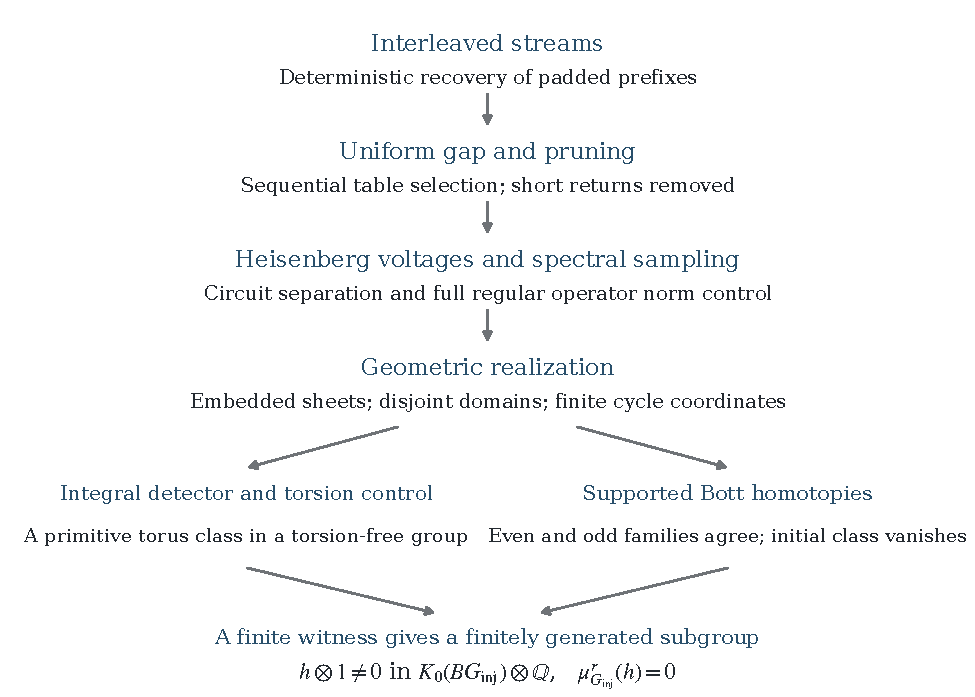
\includegraphics[width=\linewidth]{figures/proof-dependencies.pdf}
  \caption{Principal dependencies in the construction. The stream rules,
  sequential selection, and pruning precede the joint voltage and spectral
  choice. Geometric realization supports both the integral detector and
  the reduced Bott cancellation. A finite witness retains both properties
  in a finitely generated subgroup.}
  \label{fig:proof-dependencies}
\end{figure}

\subsection{Reading the construction}

There are two indices: height runs through one infinite graph tower,
while accuracy indexes a sequence of increasingly precise constructions.
The graph degree is constant across heights in any one construction and
may increase with accuracy. Section~\ref{sec:completion} records the
complete order of parameter choices after the required objects have been
defined.

Sections~\ref{sec:labeling}--\ref{sec:analysis} construct and sample the
labeled voltage tower. Sections~\ref{sec:geometry}--\ref{sec:domains}
realize it in a group and prove the cohomological detector and torsion
claims. Section~\ref{sec:assembly} establishes the reduced Bott
cancellation and extracts a finite witness. The final section puts these
conclusions together with compatible parameters and identifies the
detected torus Dirac class and its assembly image.

Throughout, all group $C^*$-algebras and all $K$-groups are complex.
Commutators mean $[a,b]=aba^{-1}b^{-1}$.  The graph construction uses
binary logarithms.  Matrix dimensions remain fixed along each
approximation sequence in which quotient $K$-theory is used; finite
generation is extracted only after an exact finite witness has been
obtained.

\clearpage
\tableofcontents
\clearpage
\section{A finite alphabet with deterministic recovery}
\label{sec:labeling}

We construct a labeled graph in layers, with the aim that every sufficiently
long immersed word has only one occurrence.  The alphabet must also remain
small relative to the incidence degrees.  The finite-alphabet separation
objective is shared with Osajda's construction
\cite[\S\S2.1--2.3, Theorem~2.7]{Osa20}; here the graph and its labels are
built together, and uniqueness will follow from explicit recovery of vertex
coordinates.

The local recovery step is elementary.  Over a finite field, subtracting
two evaluations $E_1=v+c_1u$ and $E_2=v+c_2u$ with $c_1\ne c_2$
determines $u$; either equation then determines $v$.  We apply this
observation block by block.  Labels and previously recovered neighboring
blocks will supply the evaluations.  The rules below make this process
compatible with partial terminal blocks and with comparisons between
different heights.

A \emph{slot} is a named candidate incidence at a vertex.  Once the
coefficient pools are fixed, the incidence, recovery, and vertex-deletion
assertions in this section hold for every choice of permutation tables.
Deletion fractions are counted using uniform vertex coordinates for each
fixed table realization.  The probability law on the tables is a separate
choice, made in Section~\ref{sec:expansion}.  All logarithms in this section
have base two.

The padded-stream construction and recovery scheme adapt
\cite[Sections~4 and~6]{OpenAIProjection}.  The exponents, cutoff requirements,
and gated corrections needed for the present interfaces are established
below; the projection theorem is not an existence input.

\subsection{States, families, and extra coordinates}

Fix a positive integer $b$.  Let $s$ be a sufficiently large multiple of
$20000$ and $5b$, and put
\begin{equation}\label{eq:label-parameters}
 r=\frac35s,\qquad d=2^{.40005s},\qquad
 D=2^{.60005s},\qquad q=2^{.50005s}.
\end{equation}
The numbers $d,D$ will be the two incidence degrees in a fixed slice,
and $q=\sqrt{dD}$ their geometric mean.  The exponent choices allow both
distinct coefficients for recovery and an alphabet whose square root is
small compared with $q$; the precise alphabet estimate is
\eqref{eq:sharp-alphabet} below.
These parameters stay fixed as the height $i$ varies.  They may change
when a later construction asks for a smaller approximation error.
Choose an integer $n_0\ge 10^6$, to be increased later.  For $i\ge0$ write
$bi=2s a_i+t_i$, where $0\le t_i<2s$, and define
\begin{align}
 \ell_A(i)&=r+n_0s+a_is+\max\{t_i-s,0\},\notag\\
 \ell_B(i)&=n_0s+a_is+\min\{t_i,s\},\label{eq:stream-lengths}\\
 \mathscr A_i&=\F_2^{\ell_A(i)}\times\F_2^{r+\ell_B(i)},\qquad
 \mathscr B_i=\F_2^{\ell_B(i)}\times\F_2^{s-r+\ell_A(i)}.\notag
\end{align}
The two coordinates are denoted $(u,v)$.  Regard each as an infinite bit
stream by adjoining zero coordinates.  Both coordinates on a side use
that side's block convention: an A stream has an initial block
$A_0$ of length $r$ and blocks $A_1,A_2,\ldots$ of length $s$; a B stream
has blocks $B_1,B_2,\ldots$, all of length $s$.  Index their interleaving by
\begin{equation}\label{eq:source-order}
 A_0\ (0),\ B_1\ (1),\ A_1\ (2),\ B_2\ (3),\ A_2\ (4),\ldots.
\end{equation}
For the pair of spaces at height $i$, the active coordinates of $u_A$ and
$u_B$ together form an initial segment of this interleaving.  Its length
and the logarithmic state size are
\begin{equation}\label{eq:state-sizes}
 \begin{aligned}
 L_i&=r+2n_0s+bi,&
 H_i&=L_i+s-r=(2n_0+1)s+bi,\\
 |\mathscr B_i|&=2^{H_i},&
 |\mathscr A_i|&=2^{H_i+2r-s}.
 \end{aligned}
\end{equation}
Set $m_i=H_i/\log q$.  We require, by increasing $s$,
\begin{equation}\label{eq:label-slope}
 a:=\frac b{\log q}\le10^{-6}.
\end{equation}

Let $\mathcal T$ be any fixed finite set of incidence types.  A type
$\tau$ specifies an offset $\delta_\tau\in\{-1,0,1\}$ and occurs between
$\mathscr A_i$ and $\mathscr B_{i+\delta_\tau}$ whenever both indices are
nonnegative.  Put $T=|\mathcal T|$ and
\begin{equation}\label{eq:family-modulus}
 M=2\cdot10^6s.
\end{equation}
The family of this pair is $f=(\tau,i\bmod M)$.  Thus there are at most
$TM$ families.  Its two endpoint residues, its smaller height
$h=\min\{i,i+\delta_\tau\}$ modulo $M$, and the phase of its cutoff are
determined by $f$.

For an adjacent pair, truncate the larger endpoint to the coordinate
lengths at height $h$.  Exactly $b$ coordinates are discarded: they belong
to its $u$ coordinate if that side's $u$ stream grows from $h$ to $h+1$,
and otherwise to its $v$ coordinate.  They form one interval of $b$ bits,
since $s,r$ and every active length are multiples of $b$.  Denote their
value by $e\in\F_2^b$.  For an equal-height pair let $e$ be the empty
string.  In a fixed $e$ slice, both truncated endpoint spaces are exactly
the spaces at height $h$ in \eqref{eq:stream-lengths}.

At an A endpoint a slot has serial number $j\in\{1,\ldots,d\}$; at a B
endpoint it has, in addition, a bucket $c\in\F_2^{2r-s}$.  The type is
always part of a slot name.  At the smaller endpoint of an adjacent pair,
$e$ is also part of its slot name.  At the larger endpoint it is read from
the state.  Every positive incidence is oriented from its $\mathscr A$ endpoint to
its $\mathscr B$ endpoint. A positive edge label will be
\begin{equation}\label{eq:positive-label}
 \lambda=(f,j,e,h_0),\qquad h_0=c\Vert h_0',\quad
 |h_0|=r,\quad |h_0'|=s-r.
\end{equation}
Negative labels are formal inverses.  The notation $h_0$ here is a label
head, not a height.

For each family, mark its common $u$ cutoff $L_h$ at every actual
occurrence.  Let $\kappa$ be the source-block index of the last active
common $u$ block and $t\in\{b,2b,\ldots,s\}$ its active prefix length.
Also mark the interval of extra coordinates at each adjacent occurrence.
For consecutive occurrences of one family both side lengths increase by
$Mb/2$, and the indices $\kappa$ increase by
\begin{equation}\label{eq:mark-spacing}
 K=Mb/s=2\cdot10^6b.
\end{equation}
The marked prefix length and its side therefore remain the same within
a family.  The raw $u$ data of its actual endpoint pair extend at most
one source block beyond its common cutoff.  An extra $v$ interval lies
at most two source blocks beyond that cutoff, when its coordinate blocks
are indexed by \eqref{eq:source-order}.

\subsection{Finite coefficient pools}

An A coefficient name is $(f,j,e)$, and a B coefficient name is
$(f,j,c,e)$.  We include every legal value, including values of $e$ read
from the larger state.  In particular an A name does not contain the
bucket, which has not yet been read when its label head is computed.
Let $\mathcal N_A,\mathcal N_B$ be these two finite sets.  Their sizes
satisfy
\begin{equation}\label{eq:name-count}
 |\mathcal N_A|\le TM2^b d,\qquad
 |\mathcal N_B|\le TM2^bD.
\end{equation}
Choose an injection of $\mathcal N_A$ into $\F_{2^r}$ and an injection of
$\mathcal N_A\sqcup\mathcal N_B$ into $\F_{2^s}$.  Identify these fields
linearly with their bit-coordinate spaces.  The first injection acts on
block $A_0$; the second acts on every full $s$-block.  For a name $\nu$,
write $K_\nu$ for the block-diagonal map that multiplies each block by
its assigned field element, expressed in bit coordinates.
The same coefficients are used on every repeated block.
The finite fields used here introduce no group elements: for each $h$,
the roots of $z^{2^h}-z$ in a splitting field over $\F_2$ form a field
of $2^h$ elements, since the polynomial has derivative $-1$ and its
roots are closed under the field operations.

Distinct coefficients make the two-evaluation recovery step possible.
Expansion requires a second property: after restricting to an active
prefix, no output functional should give the same input functional on
too many slots.  The next lemma supplies this multiplicity bound as well
as distinctness; Section~\ref{sec:expansion} uses it to estimate the mean
incidence operator.

\begin{lemma}[Coefficient choice]\label{lem:coefficient-pools}
For sufficiently large $s$, the injections can be chosen so that, within
every fixed family and extra slice and on either side, the following
holds.  If $n$ is its number of slots, $\zeta$ is any nonzero output
linear functional on an ordinary $s$-block, and $b\le t\le s$, then each
restricted input functional
\[
  (\zeta K_\nu)|_{\F_2^t}
\]
occurs on at most $2^{1-b}n$ slots.  All distinct names have distinct
coefficients in every field in which they occur.
The analogous bound holds on the initial A field for every prefix
length between $b$ and $r$.
\end{lemma}

\begin{proof}
The injections exist because the polynomial factor $TM$ and fixed factor
$2^b$ in \eqref{eq:name-count} are dominated by the positive exponent
gaps $r-.40005s$ and $s-.60005s$.  Choose both injections uniformly.
For fixed nonzero $\zeta$, multiplication identifies the field
coefficients bijectively with all output-to-input functionals.  On any
specified set of $n$ names these are therefore sampled without
replacement.  Restriction to $t$ input bits has fibers of proportion
$2^{-t}\le2^{-b}$.

Here is the required tail estimate.  For $n$ zero--one samples without
replacement, with sum $S$ and mean success proportion $p$, one has
\[
 \mathbb E\exp(u(S-np))\le\exp(nu^2/8).
\]
Indeed the exponential moment before centering is an elementary
symmetric mean in the population entries $1,e^u$.  Replacing two unequal
nonnegative entries by their average increases every elementary
symmetric sum: the only changing term is their product multiplied by
a nonnegative symmetric sum in the other entries.  Iteration compares
the moment with sampling with replacement.  For a centered Bernoulli
variable, the second derivative of the logarithmic moment generating
function is a tilted variance, at most $1/4$; integrating twice proves
the displayed bound.  Exponential Markov inequality gives
\[
 \Pr\{S-np\ge 2^{-b}n\}\le
 \exp(-2^{1-2b}n).
\]
There are at most $s2^{2s}$ choices of an output functional, prefix length,
and restricted value.  Multiplying by the polynomial number of families
and the fixed number of extra slices and sides still gives $2^{O(s)}$
tests.  Each has $n\ge d=2^{.40005s}$.  Their total failure probability
tends to zero.  Fix a choice for which none fails.
\end{proof}

\subsection{Universal corrections and permutation rules}

The edge equations will couple each affine evaluation to a permuted
input block at the opposite endpoint.  To compare occurrences at different
heights, we use one system of equations on arbitrary padded streams.
The corrections remove the extra coordinates of an adjacent-height pair,
while the gates and identity blocks preserve the padded tail.  Their
dependence on earlier raw inputs is what will let recovery proceed one
block at a time.

We now specify these rules on arbitrary padded raw $u_A,u_B$ streams,
not only on actual endpoint states.  A pair of full raw blocks means
$(B_j,A_j)$ for $j\ge1$.  For a source-block index $k>20$, put
$J(k)=\lfloor(k-5)/2\rfloor$ and let
\begin{equation}\label{eq:lag-gate}
 g_k=1\quad\Longleftrightarrow\quad
 (u_{B,J(k)-3},u_{A,J(k)-3},\ldots,
   u_{B,J(k)},u_{A,J(k)})\ne0.
\end{equation}
For $k\le20$ put $g_k=1$.  Thus every noninitial gate reads exactly
eight full raw blocks and reads no source-block index greater than
$k-5$.  In particular a correction to an evaluation block cannot
consult the source block that will be recovered from that evaluation.

Fix a positive label \eqref{eq:positive-label}.  At every marked extra
interval of its family, XOR $e$ into that raw coordinate interval if
$g_k=1$, where $k$ is the coordinate-block index containing the interval.
There are no corrections for an equal-height family.  Denote the resulting
streams by
\begin{equation}\label{eq:corrected-streams}
 \bar u_C=u_C+C^u_{C,\lambda},\qquad
 \bar v_C=v_C+C^v_{C,\lambda},\qquad C\in\{A,B\}.
\end{equation}
The sums are XOR sums; each finite prefix uses finitely many disjoint
marked intervals.  Every correction offset in a block is determined by
the label and raw $u$ blocks strictly before both blocks coupled by the
edge equation below.  This extra lag is deliberate.

For every family, label, source-block index $k$, and tuple of all raw $u$
blocks strictly earlier than $k$ in \eqref{eq:source-order}, provide a
permutation table.  At an unmarked index it is a permutation of the full
block; at a marked cutoff with active length $t$ it is a permutation of
$\F_2^t$.  These are distinct variables for distinct complete keys.  There
are finitely many variables at each source-block index.

The transformation at a source block is defined as follows.
\begin{enumerate}
\item At each marked cutoff use its prefix table on the first $t$ bits
and the identity on the suffix, if $g_k=1$; if $g_k=0$, use the identity
on the entire block.
\item At the twenty source blocks immediately following every marked
cutoff, use the identity unconditionally.
\item At every other source block use its full-block table if $g_k=1$,
and otherwise the identity.
\end{enumerate}
The marked and following intervals do not overlap by
\eqref{eq:mark-spacing}.  Tables act on corrected $\bar u$ blocks, while
their keys and gates read raw preceding $u$ blocks.  Write
$P_{A,\lambda}(\bar u_A)$ and $P_{B,\lambda}(\bar u_B)$ for the two
transformed streams.  For a fixed slot write
$Q_C=\bar v_C+K_\nu\bar u_C$ for its corrected evaluation; the slot
and label subscripts will usually be suppressed.  Its difference from
the raw evaluation $v_C+K_\nu u_C$ is the known correction offset
$C^v_{C,\lambda}+K_\nu C^u_{C,\lambda}$.
The universal edge equations are
\begin{equation}\label{eq:universal-edge-equations}
 \boxed{\quad
 \bar v_A+K_{(f,j,e)}\bar u_A
       =h_0\Vert P_{B,\lambda}(\bar u_B),\qquad
 \bar v_B+K_{(f,j,c,e)}\bar u_B
       =h_0'\Vert P_{A,\lambda}(\bar u_A).
 \quad}
\end{equation}
They are equations of infinite padded streams.

For the auxiliary incidence at an actual pair, modify these rules at
that occurrence only: force its extra correction on, if there is one,
and force its current final-prefix permutation on.  All lower rules
retain their gates.  Denote this auxiliary prescription by a superscript
$0$.  We shall delete states for which either forced choice was necessary.
The sparse unconditional identity zones replace any need for a
post-cutoff gate that could inadvertently read the raw extra bits.

\subsection{Auxiliary incidences and uniform coordinates}

The auxiliary prescription gives a finite incidence at every height pair.
We first verify that its equations preserve the required supports, then
solve them in either direction.  The same inversion will identify the
uniform coordinates used to count gate failures.

\begin{lemma}[Inversion and uniform coordinates]\label{lem:incidence-inversion}
For every choice of tables the auxiliary prescription has exactly one
edge at every specified endpoint and slot.  In a fixed extra slice it is
biregular of degrees $d,D$.  A uniform endpoint with a fixed slot, after
fixing its extra value when necessary, is parametrized bijectively by
the free label head and all free raw $u_A,u_B$ coordinates at the common
cutoff.  Consequently those raw coordinates are independent uniform bits.
\end{lemma}

\begin{proof}
\emph{Preservation of the common support.}
At the actual larger endpoint the forced correction cancels its extra
bits.  Lower correction intervals lie in active coordinates.  Higher
correction gates vanish: their eight preceding raw blocks are wholly
beyond the actual endpoint support, because consecutive marks are
separated by $K>20$ source blocks.  Thus corrected streams have exactly
the common permitted lengths.

The transformed corrected $u$ streams preserve these lengths.  At the
last common block the suffix is the identity.  The next twenty blocks
are identity, and their corrected inputs are zero.  Raw $u$ support
extends by at most one block beyond the common cutoff.  At every later
ordinary index the gate window \eqref{eq:lag-gate} is entirely beyond
that support, so its gate is closed.  The same holds at all higher
marked rules.  This proves preservation of the padded tail, including
an extra interval in the larger endpoint's $u$ coordinate.

For clarity, the two possible common terminal shapes are
\begin{equation}\label{eq:terminal-shapes}
\begin{array}{c|cccc}
 &\ell_A&\ell_B&|v_A|&|v_B|\\ \hline
 \text{last B prefix }t&r+ns&ns+t&r+ns+t&(n+1)s\\
 \text{last A prefix }t&r+ns+t&(n+1)s&r+(n+1)s&(n+1)s+t .
\end{array}
\end{equation}
In both rows $1\le t\le s$ and the output of each block-diagonal $K$
fits in the displayed $v$ length.  If an extra interval is in $v$, it
lies beyond this output: its same-side direct block is zero there.
Thus computing $v$ from the equations cannot leak a $K u$ term into
the prescribed extra interval.

\emph{Inversion from either endpoint.}
Given an A endpoint and slot, its extra value is known, either from the
state or from the slot.  Its first $r$ evaluation bits determine $h_0$;
there are no marked corrections in the initial blocks.  Hence $c$ and
the B coefficient name are known.  Proceed through the B blocks.  To
compute its next corrected evaluation from the A endpoint, all correction
gates use already known raw blocks by their five-index lag.  The B
permutation key uses only earlier B blocks and the preceding A block.
Invert that known block permutation, then undo the known correction to
recover the next raw B $u$ block.  The other equation now determines its
raw $v$ block.  Continue in order.  The support argument just given shows
that all recovered streams have the required lengths.

Conversely a B slot gives $c$.  Its first $s-r$ evaluation bits give
$h_0'$, and hence $h_0$.  Inverting successive A block permutations
recovers raw $u_A$ and then $v_A$.  These two procedures solve the same
triangular equations and are inverse.  The lag is important here: a
correction in $Q_{B,j}$ does not read the unknown $u_{A,j-1}$, and one
in $Q_{A,j}$ does not read the unknown $u_{B,j}$.

\emph{Uniform coordinates.}
First freely specify the raw $u$ blocks on
both sides, omitting only the larger endpoint's fixed extra interval if
that interval is in $u$.  Specify $h_0$ for an A slot, or $h_0'$ for a B
slot whose bucket is fixed.  Every gate, correction, and permutation
value is now determined.  Equations \eqref{eq:universal-edge-equations}
determine both $\bar v$ streams, and undoing the corrections determines
both raw $v$ streams.  A forced extra interval in $v$ is exactly $e$.
The number of free coordinates is
\[
 \ell_A(h)+\ell_B(h)+r=\log|\mathscr A_h|
 \quad\hbox{or}\quad
 \ell_A(h)+\ell_B(h)+s-r=\log|\mathscr B_h|,
\]
respectively.  The preceding inversion proves bijectivity, not merely
equality of dimensions.  Uniform measure therefore becomes product
uniform measure in these coordinates.
\end{proof}

\subsection{Deleting gate failures}

Let $X^0$ be the union of the auxiliary incidences over all types and
height pairs.  At a slot, evaluate the natural gates on its auxiliary
edge, even where the auxiliary prescription forced them on.  If its
common last source-block index is $\kappa$, delete an endpoint state if
any of the following holds for any incident slot:
\begin{enumerate}
\item One of $g_{\kappa},g_{\kappa-1},g_{\kappa-2}$ is zero.
\item The natural gate at its actual extra correction interval is zero.
This test is omitted for equal-height pairs.
\item Among the full active A source blocks other than $A_0$, more than
$1/250$ of their gates are closed; or the same holds among the full
active B source blocks.  These are separate tests for the two parities.
\end{enumerate}
The last test counts ordinary gate closures; deterministic marked and
following identity blocks will be accounted for separately.

\begin{lemma}[Uniform gate budget]\label{lem:gate-deletions}
For every fixed set of tables, the fraction deleted for gate reasons
from either state space at any height is at most
\begin{equation}\label{eq:gate-budget}
 \varepsilon_{\rm gate}=600T2^bD\,2^{-8s}.
\end{equation}
On a surviving edge both auxiliary forced choices were unnecessary, so
the edge satisfies the universal padded equations
\eqref{eq:universal-edge-equations}.  At each surviving slot, separately
among its full A source blocks and its full B source blocks, fewer than
$.005$ of the updates are unavailable because of a closed gate or a
marked or following deterministic identity rule.  The last three source
gates and the actual prefix gate are open.
\end{lemma}

\begin{proof}
Fix a slot and, where necessary, condition on its actual extra value.
Every gate tested at or before the common cutoff, and the gate of the
extra interval at most two blocks later, reads eight full free raw
$u$ blocks.  They are independent uniform by
Lemma~\ref{lem:incidence-inversion}.  Thus each noninitial gate is closed
with probability exactly $2^{-8s}$.  Initial gates are never closed.
Each parity in the third test has at least $n_0$ full active blocks.
Linearity of expectation and Markov's inequality give probability at
most $250\,2^{-8s}$ for each of its two failures.  The first two tests
add at most $4\,2^{-8s}$.  There are at most $T2^bD$ slots at either
endpoint, since $D\ge d$.  A union bound proves
\eqref{eq:gate-budget}, with room in the constant.  Averaging over the
extra value gives the same bound at a larger endpoint.

The first two tests refer only to raw coordinates obtained before the
forced choices can matter.  If they pass, the auxiliary and universal
rules coincide along this edge; the padding argument of
Lemma~\ref{lem:incidence-inversion} applies to both ends.  Restricting to
edges with two surviving endpoints therefore gives a subgraph satisfying
the universal equations.

For either source parity, the fraction of full active blocks belonging
to marked or following twenty-block zones is at most
\[
 \frac{22}{K}+\frac{22}{n_0}<10^{-4}.
\]
Indeed these zones have at most eleven indices of each parity, are
separated by $K$ interleaved indices, and there is at most one boundary
zone in the count.  The displayed larger constants cover both endpoints
of the counting interval.  Together with the separate $1/250$ gate
bound this is less than $.005$.  A marked partial block is counted as
unavailable for a full-$s$-bit test even if its prefix gate is open.
The current cutoff and its preceding two indices are not in a previous
marked zone, by \eqref{eq:mark-spacing}.
\end{proof}

\subsection{Recovery of arbitrary padded prefixes}

The gate deletion has made every surviving edge satisfy the same
universal equations.  We can now compare two occurrences of one label
word, even when their vertex states have different active lengths.
The distance of a position from the word's ends determines how much
of its padded state can be recovered.

For an A position put
\begin{equation}\label{eq:aligned-depths}
 \delta_A(j)=(2j+1)s\quad(j\ge0),\qquad
 \delta_B(j)=2js\quad(j\ge0).
\end{equation}
Depth $\delta_A(j)$ means both raw A streams through $r+js$ bits;
depth $\delta_B(j)$ means both raw B streams through $js$ bits.
In particular B depth zero contains no data.  The available common full
depth of a state, using only blocks in which both streams are active,
belongs to $[H_i-2s,H_i]$.  These conventions have the useful exact
identities
\begin{equation}\label{eq:depth-propagation}
 \delta_A(j)-\delta_B(j)=s\quad(j\ge0),
 \qquad \delta_B(j)-\delta_A(j-1)=s\quad(j\ge1).
\end{equation}
No $r$-dependent rounding error occurs when a coherent junction is
trimmed by one edge at each end.

The radius of a position on a path is its smaller distance in edges to
the two endpoints.  A path is immersed if it does not immediately
traverse an edge and then its reverse.

\begin{lemma}[Padded-prefix recovery]\label{lem:tower-recovery}
Let two immersed paths in the gate-surviving graph have the same
oriented label word.  At corresponding A positions of radius at least
$2j+1$, both raw streams agree through $r+js$ bits.  At corresponding B
positions of radius at least $2j$, both raw streams agree through $js$
bits.  These statements compare padded coordinates, so the positions
may have arbitrarily different heights.
\end{lemma}

\begin{proof}
The label orientation identifies the side, and the complete label
identifies the family, both coefficient names, the extras, and every
universal rule.  At an interior vertex the two incident coefficient
names are distinct.  Otherwise, at A their family, serial and actual
extra agree, and at B their bucket agrees as well; they are the same
slot.  The unique-edge assertion in Lemma~\ref{lem:incidence-inversion}
would then make the path backtrack.

For either incident name $\nu$, rearrange its current corrected
evaluation block as
\begin{equation}\label{eq:recovery-linear-equation}
 v+K_\nu u=R_\nu+C^v_\nu+K_\nu C^u_\nu.
\end{equation}
If the right sides and correction offsets are known for the two names,
their difference recovers the entire raw $u$ block because the difference
of the field coefficients is nonzero.  Then either equation recovers
the raw $v$ block.  The argument applies to full padded blocks even
when an actual endpoint has only a partial active block.

At an A position of radius one, the two first evaluations are precisely
the two label heads, and the initial correction offsets vanish.  This
recovers $A_0$.  Suppose next that $j\ge1$.  At a B position of radius
$2j$, each neighbor has A radius at least $2j-1$, so its raw streams are
known through block $A_{j-1}$ by induction.  The central B streams are
already known through $B_{j-1}$.  To compute the required right side of
the second equation in \eqref{eq:universal-edge-equations} through $js$
bits, one needs only the A transformed stream through
\[
 js-(s-r)=r+s(j-1).
\]
Every key for its last needed source block uses A blocks strictly before
$A_{j-1}$ and central B blocks through $B_{j-1}$.  Its argument is the
already recovered full corrected $A_{j-1}$ block.  Its gates and all
correction offsets use still earlier raw blocks by
\eqref{eq:lag-gate}.  Thus the two right sides are known, and
\eqref{eq:recovery-linear-equation} recovers $B_j$.

At an A position of radius $2j+1$, both neighbors have B radius $2j$.
The first edge equation through $r+js$ uses the B transformed stream
through $js$.  Its last argument is the already recovered corrected
$B_j$ block, and its keys use central A blocks only through $A_{j-1}$
and earlier B blocks.  Again the correction lag makes every offset
known.  Subtraction recovers $A_j$.

This induction is an induction on individual source blocks, not on
whole A--B pairs.  At each step both table keys and table arguments
are known before any current output is used.  The universal rules
are identical in the two occurrences, including at marked cutoffs
lying beyond one actual state's support.  Padding therefore causes
no exception to the induction.
\end{proof}

Figure~\ref{fig:stream-causality} summarizes this induction.
\begin{figure}[tbp]
  \centering
  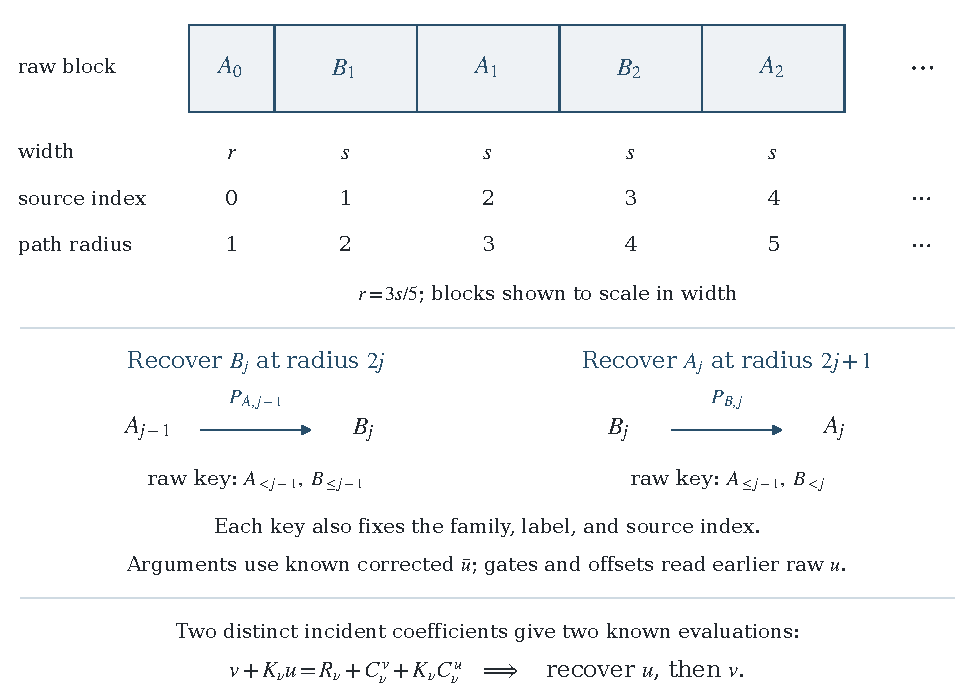
\includegraphics[width=\linewidth]{figures/stream-causality.pdf}
  \caption{Interleaving and the recovery induction of
  Lemma~\ref{lem:tower-recovery}. The radius shown suffices to recover both
  raw streams through that side's indicated block. Each arrow supplies an
  evaluation from a recovered neighbor block; two incident coefficients
  recover the receiver's $u,v$. Key abbreviations denote raw $u$ blocks.
  At the first B step, $h'_0$ supplies the initial $s-r$ evaluation bits.
  Tables act on corrected arguments; keys and gates read earlier raw
  inputs, with the lag in \eqref{eq:lag-gate}.}
  \label{fig:stream-causality}
\end{figure}

\subsection{Separating all heights}

Recovery will determine the complete state at a midpoint once a word is
long enough.  It does not yet identify the height: a shorter state might
agree with the padded prefix of a longer one.  The following deletion
excludes precisely the zero extensions needed for that ambiguity.

Put $\eta_{\rm sep}=1/2500=.0004$.  For a vertex on side $C$ at height $i$, and
each $i'<i$ with $i'\equiv i\pmod M$, let
\begin{equation}\label{eq:separation-interval}
 \Delta=\ell_C(i)-\ell_C(i')=(i-i')b/2,\qquad
 q(i,i')=\left\lfloor\min\{\eta_{\rm sep} H_{i'},\Delta\}\right\rfloor.
\end{equation}
Delete the vertex if its $q(i,i')$ raw $u_C$ bits immediately following
the smaller cutoff $\ell_C(i')$ are all zero.  These are active bits
at height $i$.  Denote by $X^{\rm good}$ the graph induced from $X^0$
after the gate and separation deletions.

\begin{lemma}[Uniform separation budget]\label{lem:separation-deletions}
The fraction deleted for separation from either side at any height is
at most
\begin{equation}\label{eq:separation-budget}
 \varepsilon_{\rm sep}
 =2\left(
 \frac{2^{-Mb/2}}{1-2^{-Mb/2}}
 +\frac{2^{-\eta_{\rm sep} H_0}}{1-2^{-\eta_{\rm sep} b}}
 \right).
\end{equation}
\end{lemma}

\begin{proof}
Uniform raw vertex coordinates are independent bits.  The probability
of the test for $i'$ is $2^{-q(i,i')}$.  The elementary inequality
\[
 2^{-\lfloor\min(x,y)\rfloor}\le2(2^{-x}+2^{-y})
\]
splits its bound into a term depending on the smaller height and one
depending on the height difference.  Summing the latter over positive
multiples of $M$, and the former even over all nonnegative smaller
heights, gives \eqref{eq:separation-budget}.  Both sums converge
uniformly in the larger height.
\end{proof}

\begin{proposition}[The deterministic labeled tower]\label{prop:tower-labels}
For every fixed finite type set and every sufficiently large $s$ as
above, the construction has the following properties.
\begin{enumerate}
\item The auxiliary state sizes are \eqref{eq:state-sizes}.  In a fixed
extra slice an incidence has degrees $d,D$.  Without slicing, its
smaller side acquires the extra factor $2^b$ and its larger side does
not.  The total degrees are at most $T2^b d$ on A and $T2^bD$ on B.
\item The labeling is folded: no two outgoing oriented edges at a
vertex have the same label.  Its signed alphabet satisfies
\begin{equation}\label{eq:sharp-alphabet}
 |\mathcal S|\le 2TM2^b d2^r,
 \qquad
 \frac{\sqrt{|\mathcal S|}}q
 \le 2^{-.000025s+O(\log s)+O_{T,b}(1)}\longrightarrow0.
\end{equation}
\item At every height the fraction of removed vertices on each side is
at most $\varepsilon_{\rm gate}+\varepsilon_{\rm sep}$.  This bound can
be made arbitrarily small, uniformly over heights and all table choices.
The separate-parity and terminal gate conclusions of
Lemma~\ref{lem:gate-deletions} hold.
\item Every immersed path in $X^{\rm good}$ starting at height $i$ and
having length at least $\lceil1.002m_i\rceil$ is the unique immersed
path with that oriented word anywhere in $X^{\rm good}$.  This is a
global assertion over all heights and components.
\end{enumerate}
\end{proposition}

\begin{proof}
The degree statements follow from
Lemma~\ref{lem:incidence-inversion}.  At a larger endpoint, a fixed
state specifies its extra value; at a smaller endpoint that value
ranges over its slots.  At an A endpoint equal labels specify equal
serial, family, and extra, hence the same slot.  At B they also specify
the bucket.  Uniqueness of the edge at a slot proves foldedness, and
restriction to an induced subgraph preserves it.  Counting
\eqref{eq:positive-label} gives \eqref{eq:sharp-alphabet}; its exponent
uses $\log d+r=1.00005s$, not a coarser word-counting bound.
The deletion assertions are
Lemmas~\ref{lem:gate-deletions} and~\ref{lem:separation-deletions}.

For fixed $b$ and incidence types, the label count has logarithm at most
$1.00005s+O(\log s)$, whereas $\log_2(q^2)=1.0001s$.
This strict margin persists after fixed finite refinements of the labels.
It will make the weighted forest error tend to zero in
Lemma~\ref{lem:finite-profile-realization}.

It remains to prove global uniqueness.  Let
$N=\lceil1.002m_i\rceil$ and compare the first $N$ edges of two paths
with the same oriented word.  Their midpoint radius is at least
$\lfloor N/2\rfloor$.  If the first midpoint has height $j$, then
\[
 H_j\le H_i+bN\le(1+1.002a)H_i+b.
\]
By Lemma~\ref{lem:tower-recovery}, their common recovered aligned depth
$\delta$ satisfies
\[
 \delta\ge s(N/2-2)
 \ge\frac{1.002}{1.0001}H_i-2s
 \ge1.001H_j.
\]
The last inequality follows from $a\le10^{-6}$,
$H_i\ge(2\cdot10^6+1)s$, and $b/s=.50005a$.

For all heights, \eqref{eq:stream-lengths} gives
\begin{align*}
 \ell_A&\le H/2+.1s,& |v_A|&\le H/2+.6s,\\
 \ell_B&\le H/2,& |v_B|&\le H/2+.5s.
\end{align*}
An aligned A depth $\delta$ recovers $\delta/2+.1s$ bits of each
stream, and a B depth recovers $\delta/2$ bits.  Since $H_j\ge1000s$,
the displayed recovery covers the entire first midpoint state.

The labels give equal height residues at the two midpoint positions.
If their heights differ, write $i_-<i_+$ for them.  Their own-$u$
length difference is the $\Delta$ of
\eqref{eq:separation-interval}.  The smaller state's padding is zero
on the interval tested there at the larger state.  Its endpoint is at
most
\[
 (1/2+\eta_{\rm sep})H_{i_-}+.1s\quad\text{on A},\qquad
 (1/2+\eta_{\rm sep})H_{i_-}\quad\text{on B}.
\]
Because $H_{i_-}\le H_j$ and $2\eta_{\rm sep}<.001$, the recovered prefix
contains that whole interval, even if $i_+$ is arbitrarily large.
The larger state would therefore have failed its separation test,
a contradiction.  The two heights are equal.  Their entire states
agree by the recovery already proved.  Foldedness now identifies the
paths in both directions from this midpoint, and uniquely continues
any longer common word.
\end{proof}

\subsection{The interface with probabilistic selection}

\begin{remark}[Terminal dimensions]\label{rem:terminal-dimensions}
The two rows of \eqref{eq:terminal-shapes} give the exact terminal
dimension split needed later.  In the side containing a partial final
$u$ block, its final pair $(u,v)$ has dimensions $(t,s)$; the other side
has a final pair of dimensions $(0,t)$.  Two independent incident
evaluations impose respectively $s-t$ and $t$ compatibility bits.
The first assertion follows because multiplication by a nonzero
coefficient difference is injective on the active $t$-dimensional
subspace.  The second is simply equality of the two $t$-bit evaluations.
Thus the sum is exactly $s$.  For adjacent incidences first move each
known affine correction $C^v+K C^u$ intact to the other side of its
evaluation equation.  A change in one input bit can affect all output
coordinates under field multiplication; these known shifts cost no
random dimension.  Only the width of the common active random prefix
can cost compatibility bits.  Projection to such a prefix of width
$w'$ gives an image of dimension at most $w'+t$ in $2w'$ dimensions,
hence codimension at least $\max\{0,w'-t\}$.  The adjacent-cutoff and
block-boundary cases, including a newly deterministic fragment, are
proved in Lemma~\ref{lem:pruning-terminal-codimension}; they lose at
most $4b$ compatibility bits.  No injectivity of a truncated
coefficient difference is asserted.
The probabilistic use of these dimensions still requires distinct
current table variables; that issue is addressed in
Proposition~\ref{prop:pruning}.
\end{remark}

\begin{remark}[Inputs to the probabilistic stages]\label{rem:label-interface}
The uniform-coordinate statement is an assertion for each fixed table
realization.  Proposition~\ref{prop:sequential-law} may therefore choose
the tables successively while retaining all deletion budgets.  The current
tables are coordinatized in
Lemma~\ref{lem:fresh-matching-coordinates} below; they are independent
under the product reference law used there.  In reconstruction of a
fixed labeled candidate, endpoint free $u$ bits are enumeration data
fixed before sampling.  At update $B_j$ the queried argument of
$P_{A,j-1}$ is already known; at the following update $A_j$ the
argument of $P_{B,j}$ is already known.  Current untested outputs can
affect only later arguments.  Gates for XOR corrections use the
stronger lag \eqref{eq:lag-gate}; ordinary preceding-key dependence
alone would not suffice for those corrections.
\end{remark}

\section{Expansion and the sequential probability law}
\label{sec:expansion}

We now choose the permutation tables to make every auxiliary incidence
expand.  The choice must also retain a quantitative probability estimate
for pruning: at one source-block update, conditioning on expansion may
increase the probability of a joint test of $k$ current tables by at most
$e^{\varepsilon_s k}$, where $\varepsilon_s\to0$ as $s\to\infty$.
Proposition~\ref{prop:sequential-law} supplies both conclusions for one
law on the full tower.  The expansion bound concerns the auxiliary
incidences before vertex deletions.

Throughout the finite estimates, fix a family at a marked cutoff, all
its earlier tables, and one extra-bit slice.  Only its current
active-prefix tables are random, and the reference law makes them
independent uniform permutations.  The auxiliary prescription forces
the current gate open.  We first bound the mean incidence operator,
then select tables for which all cuts expand, controlling the change of
law at the same time.  Every bound is uniform in the earlier history
and the height; this uniformity will permit successive choices along
the tower.

Put $\theta=2^{1-b}$.  Choose the fixed integer $b$ sufficiently large
that $\sqrt{5\theta}<3/5$.  All averages on either vertex side are
probability averages.  For one fixed-extra slice, write $A,B$ for its
common-cutoff coordinate spaces and define
\[
 (Nf)(a)=\frac1d\sum_{e:e^-=a}f(e^+),\qquad
 (N^*g)(b')=\frac1D\sum_{e:e^+=b'}g(e^-).
\]
The sums count slots, including parallel edges.  Since $d|A|=D|B|$,
these are adjoint contractions that preserve constants.  Let
$\mathsf{M}=\mathbb E N$, where the expectation is only over the current tables.
The same statements hold for $\mathsf{M}$.

\subsection{The current matching variables}

The triangular coordinates from Section~\ref{sec:labeling} identify
exactly what the current random permutations match.  Slots are the
objects in these matchings; different slots of one physical vertex
remain distinct.

\begin{lemma}[Fresh matching coordinates]\label{lem:fresh-matching-coordinates}
Fix a family occurrence, an extra slice, and every table before its last
common source block.  Under the independent uniform current-table law,
its auxiliary incidence is randomized by independent
perfect matchings between pairs of clusters of $2^t$ slot incidences, one
matching for each full final-prefix table key.  Each possible edge in a
cluster pair is permitted.  No later table affects this incidence.
\end{lemma}

\begin{proof}
Fix the serial number, full label head and preceding raw $u$ blocks.  If
the last common block is B, its remaining B data are exactly the $t$
bits of raw $u_B$ in that block; the known correction merely translates
them.  Its remaining A data are exactly the corresponding $t$ evaluation
bits.  All other coordinates are determined by
Lemma~\ref{lem:incidence-inversion}.  The forced-on current prefix table
is an arbitrary bijection between these two $2^t$-element sets.
Different complete keys specify disjoint clusters of slot incidences.
The A-terminal case reverses the roles.  The padding proof in
Lemma~\ref{lem:incidence-inversion} shows that higher tables never act on
this incidence.
\end{proof}

\subsection{A conditional Fourier estimate}

The coefficient multiplicity bound gives cancellation when we average
the evaluations $V+K_aU$ over slots.  We use the following conditional
form so that earlier raw prefixes and their correction offsets may be
held fixed.

\begin{lemma}\label{lem:conditional-fourier}
Conditional on data $C$, let $U\in\F_2^t$ and $V\in\F_2^w$ be
independent uniform vectors, independent also of auxiliary data $W$.
For $a$ in a set of $q_0$ slots let $K_a:\F_2^t\to\F_2^w$ be linear,
let $o_a=o_a(C,W)$, and let $f_a(C,z)$ have no separate dependence on
$U,V,W$.  Suppose every class of slots with a common value of
$\zeta K_a$, for any nonzero functional $\zeta\in(\F_2^w)^*$,
has at most $\theta q_0$ members.  Set
\[
 F=\frac1{q_0}\sum_a f_a(C,V+K_aU+o_a),\qquad
 \mu(C)=\frac1{q_0}\sum_a2^{-w}\sum_z f_a(C,z).
\]
Then $\mathbb E(F\mid C,W,U)=\mu(C)$ and
\begin{equation}\label{eq:fourier-conditional-bound}
 \mathbb E|F-\mu(C)|^2
 \leq\theta\,\mathbb E\left[\frac1{q_0}\sum_a2^{-w}
                       \sum_z|f_a(C,z)|^2\right].
\end{equation}
\end{lemma}

\begin{proof}
Translation of uniform $V$ proves the mean assertion.  Fix $C,W$ and
write $\widehat f_a(\zeta)=2^{-w}\sum_z f_a(C,z)(-1)^{\zeta z}$.
Orthogonality, first in $V$ and then in $U$, gives
\[
 \mathbb E_{U,V}|F-\mu(C)|^2
 =\frac1{q_0^2}\sum_{\zeta\ne0}\sum_{\mathcal C}
       \left|\sum_{a\in\mathcal C}(-1)^{\zeta o_a}
                          \widehat f_a(\zeta)\right|^2,
\]
where $\mathcal C$ ranges over classes with equal $\zeta K_a$.
Cauchy--Schwarz bounds each square by
$|\mathcal C|\sum_{a\in\mathcal C}|\widehat f_a(\zeta)|^2$.
The multiplicity assumption and Parseval's identity prove the result
after integration over $C,W$.  In particular, integration over $W$
introduces no variance of the conditional mean.
\end{proof}

The coefficient pools of Section~\ref{sec:labeling} give this
multiplicity bound on every full block and every active initial part of
length at least $b$.  The first $A$ block has length $r$; all subsequent
blocks have length $s$.  The divisibility choices make every nonempty
terminal initial part have length at least $b$.

We record why the right side of
\eqref{eq:fourier-conditional-bound} is bounded by the original input
norm in its applications.  A uniform vertex with a uniform incident
slot has a uniform neighbor, counted with the appropriate multiplicity.
Consequently the slot average of squared neighbor values is exactly the
squared input norm.  Averaging any still random table values can only
decrease this quantity, by Jensen's inequality.  Finally $V$ makes the
evaluation argument uniform conditional on all other data.  Thus the
individual Fourier norms in the Lemma are precisely bounded by these
slot norms; no factor depending on the number of blocks is introduced.

\subsection{Two interacting prefix bands}

To apply the Fourier estimate to the whole incidence, decompose a
function into orthogonal increments as longer state prefixes are revealed.
Triangular inversion couples only two neighboring levels of these
prefix decompositions.  The only additional estimate is at the terminal
block, where the current prefix permutation supplies the missing
average.

Let $P_h^A$ be expectation onto the first $r+hs$ bits of both raw
$A$ coordinates, and let $P_j^B$ be expectation onto the first $js$
bits of both raw $B$ coordinates.  Padded coordinates are deterministic
zero.  The filtrations therefore terminate at the identities.  In
particular $P_0^B=C_B$, the projection onto constants.  Write $C_A$
for the corresponding projection on $A$.

For a fixed $A$ slot, a function in $\operatorname{ran}P_j^B$ can
be evaluated at its neighbor using only
\begin{equation}\label{eq:forward-prefix-data}
 u_A[0,r+(j-1)s),\qquad Q_A[0,r+js).
\end{equation}
The first $r$ evaluation bits give the label head.  Successive inversion
of the triangular permutations then gives $u_B$ through its $j$th
block; the equation for $Q_B$ uses $u_A$ only through its $(j-1)$st
block to give $v_B$ through length $js$.
In the reverse direction, a fixed $B$ slot evaluates a function in
$\operatorname{ran}P_h^A$ using only
\begin{equation}\label{eq:reverse-prefix-data}
 u_B[0,hs),\qquad Q_B[0,(h+1)s).
\end{equation}
Here the bucket is already specified by the slot.  The remaining head
and then $u_A$ are recovered from the evaluation bits, and the equation
for $Q_A$ gives the required $v_A$ bits.

These descriptions also apply to the corrected coordinates.  Their
extra bits are fixed in the slice.  Every correction gate ends before
both coupled blocks, so its offset is determined by the preceding raw
prefix.  The same is true of an ordinary permutation gate.  A current
gate is forced open, hence constant.  No unknown current raw input
enters a key for its own source block.  The identity suffix at a mark
and the prescribed subsequent identity blocks make the assertions
valid beyond an actual cutoff as well.  These are the reasons for
using raw prefixes in the keys and the lag specified in
Section~\ref{sec:labeling}.

Since multiplication is block diagonal, there is no spill into a
following evaluation block.  Equations
\eqref{eq:forward-prefix-data}--\eqref{eq:reverse-prefix-data} imply
\begin{equation}\label{eq:two-prefix-bands}
 \operatorname{ran}(\mathsf{M}P_j^B)\subseteq\operatorname{ran}P_j^A,
 \qquad
 \operatorname{ran}(\mathsf{M}^*P_h^A)\subseteq\operatorname{ran}P_{h+1}^B.
\end{equation}
They hold before as well as after averaging current tables.
For every full interval that is active, Lemma~\ref{lem:conditional-fourier}
also gives
\begin{align}
 \|(1-P_{j-1}^A)\mathsf{M}P_j^B\|^2&\leq\theta,
       \label{eq:forward-full}\\
 \|(1-P_h^B)\mathsf{M}^*P_h^A\|^2&\leq\theta.
       \label{eq:reverse-full}
\end{align}
For \eqref{eq:forward-full}, condition on the preceding $A$ prefix.
The new data in \eqref{eq:forward-prefix-data} occur solely as
$V+K_aU+o_a$, with $U$ the new $A$ input block and $V$ its evaluation
block of $v_A$ bits.  The direct input in that equation stops before
$U$.  The $A$ coefficient does not depend on the unknown bucket in
the head.  For \eqref{eq:reverse-full}, condition on $P_h^B$ and use
the next $B$ input and evaluation blocks.  This time the direct input
in \eqref{eq:reverse-prefix-data} again stops before $U$; the slot
already fixes the bucket, and its coefficient does not depend on the
unknown suffix of the head.  Thus neither application has a separate
dependence on the fresh $U$.  The slot-norm argument above completes
both estimates, including $h=0$.

\begin{lemma}[The conditional mean]\label{lem:conditional-mean}
For every fixed earlier-table history, every marked cutoff, and every
extra-bit slice,
\[
 \|\mathsf{M}:1_B^\perp\longrightarrow1_A^\perp\|
       \leq\eta:=\sqrt{5\theta}<3/5.
\]
The same bound holds for the complete adjacent-height incidence.
\end{lemma}

\begin{proof}
\emph{The full blocks.}
Use the orthogonal difference projections
\[
 E_0^A=P_0^A-C_A,\quad E_h^A=P_h^A-P_{h-1}^A\ (h\geq1),
 \qquad E_j^B=P_j^B-P_{j-1}^B\ (j\geq1).
\]
Equation~\eqref{eq:two-prefix-bands} implies
$E_h^A\mathsf{M}E_j^B=0$ unless $h\leq j\leq h+1$.
The band $h=j$ is bounded by \eqref{eq:forward-full}, and the band
$j=h+1$ by the adjoint of \eqref{eq:reverse-full}, whenever the
blocks in question are full.  Within either band the input spaces
are mutually orthogonal, as are the output spaces.  Each band
therefore has norm at most $\sqrt\theta$, and their sum at most
$2\sqrt\theta$.

\emph{The terminal block.}
There are two possible terminal forms.  If the final input block is
a $B$ block, write
\[
 \ell_A=r+ns,\quad \ell_B=ns+t,\qquad
 |v_A|=r+ns+t,\quad |v_B|=(n+1)s,\quad b\leq t\leq s.
\]
For the input differences with $1\leq j\leq n$, all blocks required
in both bands are full, and consequently
\begin{equation}\label{eq:low-B-mean}
 \|\mathsf{M}(P_n^B-C_B)\|\leq2\sqrt\theta.
\end{equation}
Fix a $B$ slot.  Inversion through the preceding blocks determines
all of $u_A$ and all but the last $t$ bits of $v_A$ using
$u_B[0,ns)$ and $Q_B[0,(n+1)s)$.  The current prefix permutation
uniformly averages the remaining $t$ bits of $Q_A$.  Its coefficient
term $K_Au_A$ ends at $r+ns$, so these are exactly the remaining
$v_A$ bits, up to a known correction.  The matching key contains
only the label and preceding raw inputs.  After this average, its
slot value has no separate dependence on the last $t$ raw $u_B$
bits.  Conditional on $P_n^B$, it is therefore a function of
$V+K_aU+o_a$, with $U\in\F_2^t$ and $V\in\F_2^s$.
Lemma~\ref{lem:conditional-fourier} gives
\[
 \|(1-P_n^B)\mathsf{M}^*\|^2\leq\theta.
\]
Combining this orthogonally with the adjoint of
\eqref{eq:low-B-mean} gives $\|\mathsf{M}^*g\|^2\leq5\theta\|g\|^2$
for centered $g$.

If the final input block is an $A$ block, the lengths are instead
\[
 \ell_B=(n+1)s,\quad \ell_A=r+ns+t,\qquad
 |v_A|=r+(n+1)s,\quad |v_B|=(n+1)s+t.
\]
The full-block argument on $E_h^A$, $0\leq h\leq n$, gives
$\|\mathsf{M}^*(P_n^A-C_A)\|\leq2\sqrt\theta$.
The current permutation averages the final $t$ evaluation bits of
$Q_B$, on which $K_Bu_B$ is zero.  Conditional on $P_n^A$, the
remaining slot function depends on the final $t$ input bits of $A$
only through their full $s$-bit evaluation.  Hence
$\|(1-P_n^A)\mathsf{M}\|^2\leq\theta$, and the same orthogonal combination
proves the assertion.  Both arguments include $t=s$; the initial
$r$-block is never terminal because the tower starts after many
complete pairs.

\emph{Combining the extra-bit slices.}
If the larger side
is $A$, its space is $A_0\times\F_2^b$ and the complete operator
has components $\mathsf{M}_e$.  For centered $f$ on $B$,
$\|\mathsf{M}f\|^2=\mathbb E_e\|\mathsf{M}_ef\|^2\leq\eta^2\|f\|^2$.
If the larger side is $B$, use the adjoint version of this argument.
Equivalently, write an input as $f_e=c_e+f_e^0$; its overall mean
zero says $\mathbb E_ec_e=0$, so the constants cancel before
Jensen's inequality is applied to $\mathbb E_e\mathsf{M}_ef_e^0$.
\end{proof}

\subsection{Cut concentration}

The mean estimate gives a lower bound for every expected cut.  The
matching coordinates now let us turn this into a failure-probability
bound for each fixed cut.

We now condition only on earlier tables and one extra-bit slice.
Lemma~\ref{lem:fresh-matching-coordinates} identifies each current
table with a uniform bijection between two fibers of slots of size
$2^t$.  Its key fixes all other endpoint coordinates.  Distinct keys
give disjoint such fibers of slots, and the current tables are
independent.  A physical vertex may occur in several fibers through
its different slots; this does not identify their permutation
variables.

Write $\deg(v)=d$ on $A$ and $D$ on $B$, and
$\vol(S)=\sum_{v\in S}\deg(v)$.  The total volume is $V_0=2d|A|$.
Let $c(S)$ count edges crossing from $S$ to its complement, with
multiplicity.  The mean random-walk operator on the union of the
two sides is the self-adjoint block operator with entries $\mathsf{M},\mathsf{M}^*$.
On the orthogonal complement of global constants its spectrum has
upper bound $\eta$; its additional bipartition eigenvector has
eigenvalue $-1$.  Applying its quadratic form to the centered
indicator of $S$ gives
\begin{equation}\label{eq:expected-cut}
 \mathbb E c(S)\geq(1-\eta)\vol(S)
                  \left(1-\frac{\vol(S)}{V_0}\right)
               \geq\frac15\vol(S)
\end{equation}
whenever $\vol(S)\leq V_0/2$.

For a current table $a$, let $Z_a$ count its matched pairs whose two
endpoints belong to $S$.  If $n_a$ is the fiber size, $u_a$ the
number of its $A$ slots in $S$, and $v_a$ the corresponding number
of $B$ slots, then $Z_a$ is hypergeometric with these parameters.
Moreover
\[
 c(S)=\vol(S)-2\sum_a Z_a,\qquad
 \sum_a u_a\leq\vol(S).
\]
For completeness, sampling $u_a$ distinct entries from a population
of $v_a$ ones and $n_a-v_a$ zeros gives, for every real $\lambda$,
\[
 \mathbb E e^{\lambda(Z_a-\mathbb EZ_a)}
       \leq e^{\lambda^2u_a/8}.
\]
Indeed the average of products of $u_a$ distinct positive numbers
is at most the $u_a$th power of their arithmetic mean: this follows
by repeatedly replacing two unequal numbers by their average in
the elementary symmetric polynomial, which increases it.  Apply
this to the numbers $1,e^\lambda$.  The resulting bound is the
moment generating function for sampling with replacement.  For
one Bernoulli variable its centered log moment generating function
has value and first derivative zero at zero and second derivative
at most $1/4$ everywhere, proving the displayed bound.
Independence and exponential Markov's inequality therefore yield
\begin{equation}\label{eq:cut-failure}
 \mathbb P\{c(S)<.05\vol(S)\}
 \leq \exp\{- .01125\vol(S)\}
 \leq \exp\{-c_0d_{\min}|S|\},\qquad c_0=10^{-3},
\end{equation}
where $d_{\min}=\min(d,D)$.  The numerical constant uses
$\sum_aZ_a-\mathbb E\sum_aZ_a>.075\vol(S)$ and the choice
$\lambda=.3$.

\subsection{The finite selection lemma and its conditioning bound}

Join two physical vertices when some choice of a current table
could join them.  This \emph{possible graph} has maximum degree
$\Delta\leq2^{C s}$, where $C$ may depend on the fixed number of
types and on $b$.  Each current table meets at most $2^{C s}$
vertices; the number of tables meeting a vertex has the same bound.
These bounds do not depend on the height.  It suffices to avoid
the cut failures in \eqref{eq:cut-failure} for nonempty connected
sets $S$ in the possible graph satisfying $\vol(S)\le V_0/2$.
In fact any failed cut of at most half the volume has a failed
connected component, since both volume and crossing add over
those components.

Let $A_S$ be such a cut-failure event.  It depends only on tables
meeting $S$.  Two events with no common table are independent,
jointly with any collection of other events using disjoint tables.
If their table sets meet, some vertex of one is within distance
two of a vertex of the other in the possible graph.  A connected
$j$-set containing a specified vertex is encoded by a walk of
length $2(j-1)$ obtained from a deterministically chosen rooted
spanning tree.  Thus the number of neighboring $j$-set events is
at most
\begin{equation}\label{eq:dependency-count}
 |S|\Delta^{2j+C_1}
\end{equation}
for an absolute enlargement $C_1$.

Assign weights $x_S=\exp(-c_0d_{\min}|S|/2)$.  Equations
\eqref{eq:dependency-count} and the exponential growth of
$d_{\min}=2^{.40005s}$ imply, uniformly in $S$,
\[
 \sum_{T\sim S}x_T
 \leq |S|\sum_{j\geq1}\Delta^{2j+C_1}e^{-c_0d_{\min}j/2}
       =|S|\delta_s,\qquad\delta_s\longrightarrow0.
\]
For sufficiently large $s$, all weights are below $1/2$ and
$2\delta_s\leq c_0d_{\min}/2$.  Consequently
\begin{equation}\label{eq:lll-criterion}
 \mathbb P(A_S)\leq x_S\prod_{T\sim S}(1-x_T).
\end{equation}

This is the finite asymmetric Lov\'asz local lemma in its product form
\cite[Theorem~1.1]{MT10}; the original symmetric lemma is due to
Erd\H{o}s and Lov\'asz \cite[\S2]{EL75}. We include the conditional-probability
induction because its quantitative conditioning bound is also needed.  For a finite family
satisfying \eqref{eq:lll-criterion}, induction simultaneously proves
positivity of avoidance probabilities and the following conditional
bound.  At a given size, positivity follows from the smaller-size
bounds by the product rule; the empty avoidance event has probability
one.  For any $A_i$ the bound is
\[
 \mathbb P\left(A_i\,\middle|\,\bigcap_{j\in J}A_j^c\right)
       \leq x_i\qquad(i\notin J).
\]
Split $J$ into the neighbors $J_1$ of $i$ and its remaining set
$J_2$.  The numerator after conditioning on avoidance in $J_2$
is at most $\mathbb P(A_i)$, by independence.  If $J_1$ is empty,
independence proves the desired bound immediately.  Otherwise the denominator
for also avoiding $J_1$ is, by the product rule and the induction
hypothesis, at least $\prod_{j\in J_1}(1-x_j)$.  The criterion
now proves the induction step.  The same product rule proves
that avoidance of every event has strictly positive probability.

We also need the standard conditional-distribution estimate for an
additional event; see \cite[Theorem~2.1]{HSS11}.  Let $B$ involve
a specified set of $k$ current tables.  Let $J_1$ be the cut events
sharing one of these tables and $J_2$ all the others.  Independence
gives
\[
 \mathbb P\left(B\,\middle|\,\bigcap_S A_S^c\right)
 \leq\mathbb P(B)\prod_{S\in J_1}(1-x_S)^{-1}.
\]
For each specified table, its at most $2^{Cs}$ vertices and the
connected-set count give
\[
 \sum_{S\in J_1}x_S
 \leq k\,2^{Cs}\sum_{j\geq1}\Delta^{2j+C_1}
                          e^{-c_0d_{\min}j/2}.
\]
It follows that, for a number $\varepsilon_s\to0$ independent of
height and earlier history,
\begin{equation}\label{eq:current-event-inflation}
 \mathbb P\left(B\,\middle|\,\text{all current cuts succeed}\right)
       \leq e^{\varepsilon_s k}\mathbb P(B).
\end{equation}
The same inequality applies to any nonnegative function of those
$k$ tables, by integration of its level sets.  It concerns a joint
test of current variables.  It does not assert a bound for the
next query after conditioning on arbitrary earlier answers from
the same block.

\subsection{A gap in every chosen incidence}

The selected cut bounds give a spectral gap by the degree-weighted
Cheeger argument; compare \cite[Lemma~3.3]{SJ89} and
Chung~\cite[Section~3, Theorem~1]{ChungCheeger}.  We include the
argument in the bipartite form needed here, keeping its normalization
and edge multiplicities.
If all the selected cuts satisfy $c(S)\geq h_0\vol(S)$ with
$h_0=.05$, the ordinary weighted spectral gap is at least
$h_0^2/2$.
For a real function $f$ of degree-weighted mean zero, choose a
weighted median $m$ and put $g_+=(f-m)_+$ and $g_-=(m-f)_+$.
Each has support of volume at most half.  Integration over the
level sets of $g^2$, for either one, yields
\[
 \sum_{\{u,v\}}|g(u)^2-g(v)^2|
       \geq h_0\sum_v\deg(v)g(v)^2.
\]
Cauchy--Schwarz and
$\sum_{\{u,v\}}(g(u)+g(v))^2\leq2\sum_v\deg(v)g(v)^2$
give
\[
 \sum_{\{u,v\}}(g(u)-g(v))^2
       \geq\frac{h_0^2}{2}\sum_v\deg(v)g(v)^2.
\]
The energy of $f$ is at least the sum of the energies of $g_+$
and $g_-$, while
$\sum_v\deg(v)(f(v)-m)^2\geq\sum_v\deg(v)f(v)^2$.
This proves the claimed gap.  Apply the argument to real and
imaginary parts for complex functions.  Bipartite symmetry sends
an eigenvalue to its negative; the only exceptional modes are
the global constant and bipartition functions.  Hence the
normalized incidence has centered singular norm at most
\begin{equation}\label{eq:uniform-incidence-gap}
 \rho=1-h_0^2/2<1.
\end{equation}
The slice-to-whole argument in Lemma~\ref{lem:conditional-mean}
also transfers this bound to adjacent-height incidences.

\subsection{Choosing the tables along the tower}

At one marked cutoff we have now obtained both a nonempty set of
expanding table choices and the bound
\eqref{eq:current-event-inflation} on conditioning to that set.  Future
tables do not affect this incidence.  We can therefore apply the same
finite choice successively at all marked cutoffs.

\begin{proposition}[Sequential selection]\label{prop:sequential-law}
There is a probability law on all the permutation tables such that
every auxiliary incidence has centered singular norm at most the
fixed number $\rho<1$ in \eqref{eq:uniform-incidence-gap}.
At each individual source-block update, conditional on all earlier
updates, any joint test of $k$ specified current tables has its
probability increased by at most $e^{\varepsilon_s k}$ relative
to independent uniform current tables.  The bound is uniform in
the earlier history and the height, with $\varepsilon_s\to0$.
\end{proposition}

\begin{proof}
Within each of the finitely many families order the source blocks
as $A_0,B_1,A_1,B_2,\ldots$.  Interleave the families by increasing
source-block index and a fixed family order.  At an unmarked
update choose all its active permutation variables uniformly.
At a marked update use the finite conditional distribution given
avoidance of its current cut failures, separately in the extra-bit
slices.  Conditional on all earlier source-block indices, the
current kernels in different families are independent, since a
family's cut conditions use only its own tables.  Thus grouping
the families into one source-block update gives the same bound,
with $k$ the total number of tested tables.  The mark separation
ensures at most one actual cutoff
per family at an update.  Lemma~\ref{lem:conditional-mean} and
\eqref{eq:lll-criterion} show that this distribution exists for
every possible preceding history, and
\eqref{eq:current-event-inflation} proves its test bound.  Blocks
prescribed to be identities have no random variables.

Each update has finitely many possible outcomes.  An independent
uniform number in $[0,1]$ can choose among them by consecutive
intervals of their conditional probabilities.  Iterating on the
countable sequence of updates constructs the asserted law.  A
future update does not change an earlier incidence: the prefix
and padding properties of Section~\ref{sec:labeling} guarantee
this.  Therefore all earlier expansion conditions persist.

When a test whose current-table choices and input arguments are
measurable from earlier updates is evaluated, all
later conditional distributions integrate to one.  Thus its
probability is governed by the current kernel just described,
without an additional conditioning on future expansion successes.
This observation is the form of sequential conditioning used
in the pruning argument below.
\end{proof}

\section{Pruning coherent returns and bicycles}
\label{sec:pruning}

We work with the random universal tables of
Proposition~\ref{prop:sequential-law}.  The coefficient pools have already
been fixed.  The graph in this Section has only old vertices and old edges;
the private completion is made later.  Write $X^{\mathrm{good}}$ for the
graph induced on the vertices surviving the gate and separation deletions
of Proposition~\ref{prop:tower-labels}.  These deletions are defined for
every realization of the tables.  A statement that a path is in
$X^{\mathrm{good}}$ will be used as a condition on the objects being
counted, never as additional conditioning of the table distribution.

All lengths in this Section count edges.  A bicycle is a finite connected
subgraph with first Betti number two and with no vertex of valence one.
After vertices of valence two are suppressed, it is a theta, a
figure-eight, or a barbell.  We need to exclude embedded bicycles; their
edge labels are automatically immersed because the ambient labeling is
folded.

Our goal, stated precisely in Proposition~\ref{prop:pruning}, is to remove
an arbitrarily small fraction of every layer while excluding short cycles
and bicycles. We first count repeated-prefix returns, which yield the
$.93m_i$ girth bound, and then use that bound to count the remaining short
thetas. Removing bicycles below $1.52m_i$ finally ensures that nonempty cyclically
reduced closed paths of length at most $6.04m_i$ are not Heisenberg laws,
the separation input needed for
the voltage choice.

\subsection{Prefix depth, fixed margins, and admissible returns}

We use the aligned depths of \eqref{eq:aligned-depths}, writing
$d_A=\delta_A$ and $d_B=\delta_B$.  Thus, for an A-vertex, agreement to depth
\[
  d_A(j)=(2j+1)s \qquad (j\geq0)
\]
means agreement of both raw streams through length $r+js$.  For a
B-vertex, agreement to depth
\[
  d_B(j)=2js \qquad (j\geq0)
\]
means agreement of both raw streams through length $js$.
Depth is measured in state bits; on the A-side it subtracts the constant
$2r-s$ from the number of specified raw bits.  This is why the common
scale in both cases is $H_i$.

Let $D(v)$ be the largest such depth for which both specified stream
prefixes are active at $v$.  The two possible terminal cutoffs give
\begin{equation}
\label{eq:pruning-available-depth}
 H_i-2s\leq D(v)\leq H_i
 \quad\text{for }v\in\mathscr A_i\sqcup\mathscr B_i.
\end{equation}
For example, if the active cutoff is inside B-block $j$, the B-input is
partial while its evaluation block is full; the largest common full
B-prefix ends at block $j-1$.  Its missing depth is between $s$ and $2s$.
On the other side the input has ended and the next evaluation block is
partial; the missing depth is between zero and $s$.  The case of a final
A-input is the same with the sides reversed.

Two equal state prefixes followed through one common outward label
propagate as
\begin{equation}
\label{eq:pruning-prefix-propagation}
  A_j\longmapsto B_j,\qquad B_j\longmapsto A_{j-1}.
\end{equation}
Here $A_j$ denotes both A-prefixes through $r+js$, and $B_j$ denotes both
B-prefixes through $js$.  Each propagation therefore loses exactly $s$
of aligned depth.  To verify the first assertion, the equal A-evaluations
through $r+js$, after removing their common label head, determine the B-input
through block $j$ by successive inversion.  The B-evaluation through block
$j$ uses only A-input blocks through $j-1$, already known.  The second
assertion follows from the other equation: the B-evaluation through $js$
determines the A-input through block $j-1$, and its A-evaluation uses earlier
B-inputs.  The correction offsets are equal because the label is equal and
their raw gate windows are earlier than both coupled blocks.  Adjacent
cutoffs do not invalidate the stated full prefixes: the cutoff moves by at
most $b<s$, whereas one propagation has removed one whole interleaved
block.  These observations prove~\eqref{eq:pruning-prefix-propagation}
also when one of the original vertices is at its last complete prefix.

We make the margin independent of the particular subpath.  For $k\geq0$
put
\[
 T_k=H_0(11/10)^k,\qquad
 I_k=[5T_k/6,6T_k/5],\qquad M_k=T_k/25.
\]
A vertex belongs to band $k$ when its height scale belongs to $I_k$.
Each height belongs to at most a fixed number of bands, independent of
$H_0$ and $s$, and
\begin{equation}
\label{eq:pruning-margin-range}
 \frac1{30}\leq\frac{M_k}{H_i}\leq\frac{6}{125}<.05
 \quad(H_i\in I_k).
\end{equation}
We shall use the weaker interval $[.03,.05]$ in numerical estimates.
If a finite old-edge subgraph through height $i$ has total length at most
$7m_i$, its scale variation is at most $7bm_i$.  For sufficiently small
$b/s$, choose $k$ with $T_k\leq H_i<T_{k+1}$.  All its vertex scales then
lie strictly inside $I_k$.  Thus every later short-path application fits
one band.  Unlike a disjoint partition into bands, this choice has room
at every endpoint.

\begin{definition}[Coherent return]
\label{def:coherent-return}
In band $k$, a coherent return is a positive-length nonbacktracking path
\[
  v_0,e_1,v_1,\ldots,e_p,v_p
\]
in $X^{\mathrm{good}}$, entirely in that band, whose endpoints are on
the same side and agree through an available aligned depth
\begin{equation}
\label{eq:coherent-threshold}
 h\geq ps/2+M_k,
 \qquad h\leq\min\{D(v_0),D(v_p)\}.
\end{equation}
It is minimal if no proper positive-length contiguous subpath is a
coherent return for the same band and the same $M_k$.
An exact closed nonbacktracking path is included whenever it satisfies
the available-depth condition.
\end{definition}

The endpoint side makes $p$ even.  For a fixed length, side, and band,
we always use the least aligned $h$ satisfying the first inequality
of~\eqref{eq:coherent-threshold}; it differs from its right-hand side by
less than $2s$.  This loses no return and removes $h$ as an extra
enumeration parameter.  Every coherent return contains a minimal one,
by choosing a shortest eligible contiguous subpath.

The threshold is chosen to make the return count smaller than a layer.
At the leading exponential scale, a length-$p$ pattern at initial scale
$H=H_i$ costs $ps$ bits of label choices and $H-h$ free endpoint bits,
while compatibility at the final active blocks imposes $ps/2$ bits of
constraints.  The
inequality $h\geq ps/2+M_k$ therefore leaves an exponent $H-M_k$,
below the layer exponent $H$.  The estimates below retain the label-rate
slack and control the losses from unequal heights, terminal cutoffs,
and the conditioned table law.

\begin{lemma}[The two junction coefficients are different]
\label{lem:coherent-junction}
At the identified endpoints of a minimal coherent return, the two
outward incident coefficient names are different.
\end{lemma}

\begin{proof}
The pools are injective on the full finite collection of family, type,
slot, and permitted extra-value names, rather than only on the slots
at a single vertex.  Hence equality of the two coefficient names gives
the same family and the same slot data.  At an A-endpoint the label head
$h_{\mathrm{lab}}$ is the first $r$ bits of its evaluation.  At a
B-endpoint its suffix is the first $s-r$ evaluation bits and its bucket
is slot data.  Equality of the raw endpoint prefixes therefore gives
the same full outward label.  Extra-dependent coefficients cause no
exception because those extra values are part of their names.

Remove one edge at each end.  By
\eqref{eq:pruning-prefix-propagation}, the new endpoints agree to
depth at least $h-s$, and the new threshold is
$(p-2)s/2+M_k$.  The prefixes are available at the new endpoints by
the same propagation statement.  The remaining subpath is still in
the same band and consists of good vertices.  If $p>2$, this is a
proper coherent return, a contradiction.  If $p=2$, the two edges
entering its middle vertex have the same outward label there, so
foldedness makes the original path an immediate backtrack.  This too
is impossible.
\end{proof}

\subsection{Reconstructing a counted object}

The count separates choices from constraints.  Once the labels and
heights are fixed, two incident evaluations reconstruct the state at
each internal vertex.  A coherent path leaves only raw u-bits beyond
the common endpoint prefix to be chosen; a theta has no free endpoint
bits.  A formal reconstruction need not lie in the prescribed state
spaces.  Its terminal coordinates must satisfy the active cutoffs, and
at a theta's two branch vertices the third incident evaluation must
agree with the first two.  These are the constraints whose probabilities
we estimate.

We record exactly what is fixed in the enumeration.  A path pattern
consists of its length $p$, initial side and height, band, edge labels,
and the choices of next height allowed by those labels.  There are at
most three choices per edge if one does not use the height residues to
determine the choice uniquely.  A theta pattern consists of three
positive branch lengths, the root position in that abstract graph,
the initial side and height, edge labels, and allowed height changes.
All slot names, coefficients, correction extras, and current cutoffs
are fixed by this information.  Patterns with inconsistent labels or
height assignments are rejected before any random table is queried.
We also reject equal coefficient names among the two incident slots
at an internal vertex or the three slots at a branch vertex.
Such a pair specifies the same incident
slot, by the injectivity of the coefficient pools.  At an actual
vertex that slot supports just one edge, so its repetition would
be an immediate backtrack or would identify two supposed branches.
No immersed path or embedded theta is lost.  At the coherent
junction the corresponding exclusion is justified by
Lemma~\ref{lem:coherent-junction}.

There is a number $L_s$ such that the number of choices of an oriented
label together with its allowed next height is at most $L_s$, and,
by increasing $s$ after the finite type data,
\begin{equation}
\label{eq:pruning-label-count}
  L_s\leq2^{1.001s}.
\end{equation}
Indeed the additional factors here are at most a fixed multiple of
the actual alphabet size.  This deliberately loose bound is used
only in counting, not in the later forest norm estimate.

For a coherent path we identify its two endpoints only through depth
$h$.  After that depth, choose all their remaining active \emph{raw}
u-bits freely and fix them as part of the pattern.  Their inactive
u-bits are fixed to zero.  There are no free v-bits.  For a theta there
are no free endpoint bits.

\begin{lemma}[Unique reconstruction and free-coordinate count]
\label{lem:pruning-reconstruction}
Fix a coherent-path pattern with different junction coefficients,
and fix its free endpoint u-bits.  For any realization of the
universal tables there is at most one assignment of vertex states
realizing that pattern as a coherent path.  If its endpoint scales
are $H_-$ and $H_+$, the number of free bits is at most
\begin{equation}
\label{eq:pruning-free-bits}
  (H_-+H_+)/2-h.
\end{equation}
For a theta pattern, there is at most one assignment of states and
there are no free bits.  During either reconstruction all inputs and
keys queried at a source block are determined before that block's
tables are exposed.
\end{lemma}

\begin{proof}
Choose two incident slots at each theta branch vertex and use the two
incident slots at every degree-two vertex.  At the coherent
junction use the two end slots through depth $h$.  At a free end
beyond $h$ use its prescribed u-block and its single incident
evaluation.

First recover every A-block $A_0$.  Its two evaluation heads are
known from the labels.  If their coefficients are $c_1\ne c_2$,
subtraction recovers the raw u-block, and then the raw v-block.
At later blocks the known correction offsets can be moved to the
right-hand sides, so the same two equations have the form
\begin{equation}
\label{eq:pruning-two-evaluations}
 v+c_1u=E_1,\qquad v+c_2u=E_2.
\end{equation}
The difference $c_1-c_2$ is a nonzero field element and is invertible
on the full padded block.  Thus these equations uniquely give
\[
 u=(c_1-c_2)^{-1}(E_1-E_2),\qquad v=E_1-c_1u.
\]
At a free endpoint, $u$ is already prescribed and the one equation
uniquely gives $v$.

The update of B-block $j$ uses the two values of $P_{A,j-1}$ at the
neighboring A-input blocks already recovered.  The subsequent update
of A-block $j$ uses $P_{B,j}$ at the B-input blocks just recovered.
Each key contains raw blocks strictly before its source block;
current correction windows end before both coupled blocks.  All
these data are known before the current table is read.  This proves
the assertion inductively in the individual source-block order
$A_0,B_1,A_1,B_2,A_2,\ldots$.

The induction is also an unambiguous \emph{formal} reconstruction
when a pattern is invalid: solve on full padded blocks, stop after
all blocks that can meet the candidate cutoffs, and then test the
required zeros, labels, and vertex conditions.  An assignment
violating an inactive-coordinate condition need not define a graph
vertex, but it causes no ambiguity in earlier query data.  Every
actual realization is reproduced by the induction, which proves
the claimed upper bounds on realizations.  Ignoring some final
validity conditions will consequently only increase our counts.

It remains to count the free endpoint u-bits.  The active interleaving
implies
\[
 r-s\leq \ell_A(i)-\ell_B(i)\leq r,
 \qquad H_i=\ell_A(i)+\ell_B(i)+s-r.
\]
Consequently
\[
 \ell_A(i)\leq H_i/2+(2r-s)/2,
 \qquad \ell_B(i)\leq H_i/2.
\]
At aligned depth $h$ an A-endpoint has specified
$(h+2r-s)/2$ u-bits, and a B-endpoint has specified $h/2$ u-bits.
Adding the two residual lengths on their common side gives
\eqref{eq:pruning-free-bits}.  A theta has two chosen evaluations
at every vertex and hence has no freely prescribed coordinate.
\end{proof}

\subsection{The probability estimate at one source block}

Let $\mathcal F_{<t}$ contain all universal tables at source blocks
strictly preceding $t$, in every family, and all fixed pattern data.
The last assertion of Lemma~\ref{lem:pruning-reconstruction} says
that keys, input arguments, gates, coefficient choices, and the
widths of current tests are $\mathcal F_{<t}$-measurable.  In
particular, no v-coordinate solved from a current evaluation is
used in a current raw-u key.

By Proposition~\ref{prop:sequential-law}, an event $B_t$ involving
$k_t$ whole current permutation tables satisfies
\begin{equation}
\label{eq:pruning-current-domination}
 \mathbb P(B_t\mid\mathcal F_{<t})
 \leq \exp(\epsilon_s k_t)
       \mathbb P_{\mathrm{prod}}(B_t\mid\mathcal F_{<t}),
 \qquad \epsilon_s\longrightarrow0.
\end{equation}
The right-hand law is the product of the indicated current uniform
permutation laws, with earlier tables held fixed.  It is legitimate
to apply this bound to a union of output prescriptions, hence to a
linear compatibility condition.  Untested entries of a table in
$B_t$ are integrated out.  The estimate is not an assertion about
the last unknown entry of a permutation after its other entries
have been prescribed.

\begin{lemma}[Predictable accumulated rank]
\label{lem:pruning-rank-process}
Suppose that, at each of finitely many source blocks, a test is
selected from $\mathcal F_{<t}$, and its product-law probability is
at most $2^{-R_t}$.  The nonnegative integers $R_t$ and $k_t$ are
$\mathcal F_{<t}$-measurable.  If an event $A$ implies that all tests
pass, that $\sum_tR_t\geq R$, and that $\sum_tk_t\leq K$, then
\[
 \mathbb P(A)\leq \exp(\epsilon_sK)2^{-R}.
\]
The event $A$ may additionally require later minimality, missed-gate
counts, and full consistency of the reconstructed vertex states.
\end{lemma}

\begin{proof}
After a failed test give the process value zero.  Otherwise multiply
its value at step $t$ by $2^{R_t}\exp(-\epsilon_s k_t)$ when that
test passes.  Conditional expectation does not increase, by
\eqref{eq:pruning-current-domination}.  The initial value is one,
so the final nonnegative variable has expectation at most one.
On $A$ its value is at least $2^R\exp(-\epsilon_sK)$, proving the
claim.  Additional final conditions are used only in this last
lower bound, not in any conditional probability.
\end{proof}

\subsection{Terminal dimensions and equality of keys}

The two-evaluation reconstruction solves for a full padded block, but
only its active coordinates may be nonzero.  At a terminal block this
restriction imposes a number of compatibility conditions determined by
the excess of evaluation bits over input bits.  We first count these
conditions, then determine when different vertices test distinct tables.

For a vertex put
\[
 \lambda_A(i)=r+\ell_B(i)-\ell_A(i),\qquad
 \lambda_B(i)=s-r+\ell_A(i)-\ell_B(i).
\]
These are its surplus evaluation lengths $|v|-|u|$.  They lie in
$[0,s]$, and
\begin{equation}
\label{eq:pruning-surplus-pair}
 \lambda_A(i)+\lambda_B(i)=s,
 \qquad
 |\lambda_A(i)+\lambda_B(j)-s|\leq b
 \quad(|i-j|\leq1).
\end{equation}
The last inequality follows because a height step changes just one
input length by $b$.

\begin{lemma}[Terminal compatibility]
\label{lem:pruning-terminal-codimension}
If both incident common cutoffs equal the receiving vertex's own
cutoff, the terminal constraints from two independent incident
evaluations have product-law probability exactly $2^{-\lambda(v)}$.
If each incident common cutoff is at most $b$ bits below that
receiver cutoff, one can test an event on those two current tables
with probability at most
\[
 2^{-\max\{0,\lambda(v)-4b\}}.
\]
The keys must be distinct between the tested edge occurrences;
the input arguments must be known before the current tables are
exposed, and the required terminal gates must be open.
Only the actual uniform active prefix of a partial permutation is
used in this statement.
\end{lemma}

\begin{proof}
Apart from the initial short block, which is never terminal, there
are two terminal forms.  If the final active input has $t$ bits in
its $s$-bit field, then its evaluation block has all $s$ bits.
The map in~\eqref{eq:pruning-two-evaluations} sends an $s$-bit v
and a $t$-bit u-subspace injectively into two $s$-bit evaluations.
Its image has dimension $s+t$, so the compatibility codimension is
$s-t$.  The nonzero coefficient difference proves injectivity on
the full field and therefore on the active subspace.

On the opposite side, the input has ended and the last evaluation
has $t$ bits.  Its two incoming values are independent uniform
$t$-bit values from the two active-prefix permutations.  Since
$u=0$, they must agree after their known offsets are removed.
This has codimension $t$.  These two surpluses add to $s$.
The boundary cases $t=0,s$ simply move the one nonzero surplus to
the other side.  This proves the equal-cutoff statement.

For adjacent incidences the correction extras are fixed label
data, and the lagged gates are determined by earlier raw blocks.
For incidence $a$ write its known correction as
$o_a=C_a^v+K_aC_a^u$ and move the whole vector $o_a$ to the other
side of the equation.  Its support may fill the output field;
translation by it costs no random dimension.  On a common active
random prefix, with coordinate projection $\pi$ and width $w'$, the
map
\[
 (u,v)\longmapsto
 \bigl(\pi(v+K_1u-o_1),\pi(v+K_2u-o_2)\bigr)
\]
has affine image of dimension at most $w'+t$ in $2w'$ bits.
Thus its codimension is at least $\max\{0,w'-t\}$.  This uses no
invertibility of a truncated multiplier.  For the terminal form
with no input, replace $t$ in this dimension count by zero.

Here are the active widths, including the boundary between blocks.
Write $t\in\{b,2b,\ldots,s\}$ for the width of the last active
block in the interleaved raw input stream at the receiver's height;
each incident common cutoff is the receiver cutoff or is $b$ bits
earlier.  If $t>b$, both evaluations of the
partial-input side occur in the preceding source block and have
the full $s$ random bits.  Their codimension is at least $s-t$.
On the evaluation-only side the common random prefix has width
at least $t-b$, giving that many compatibility bits.  If $t=b$,
the cutoff can cross a block boundary.  On the partial-input side
the preceding source block still has full random width: it is
either ordinary or the full active prefix of a marked block.
It therefore still contributes $s-b$ compatibility bits.  On the
opposite side a lower incidence can already be in its deterministic
post-mark block.  Its surplus is only $b$, so we use the certain
event and charge zero, as permitted by
$\max\{0,b-4b\}=0$.  The same reasoning applies with A and B
interchanged; $t=s$ includes the boundary represented by $t=0$
on the other side.  All retained positive-width outputs are
actual independent uniform current-table prefixes.  These bounds
are stronger than the stated conservative loss of $4b$, and prove
the probability assertion.
\end{proof}

\begin{lemma}[A repeated terminal key identifies receiver prefixes]
\label{lem:pruning-key-prefix}
Suppose two distinct tested terminal edge occurrences at the same
source block use the same table key.  Their receiving vertices
have the same side and agree in raw u and v through available
aligned depth at least
\[
  H_*-8s,
\]
where $H_*$ is the minimum scale among the vertices of the counted
path or theta.  At any nonterminal update, equality of keys
likewise identifies both receiver prefixes through the preceding
complete receiver block.
\end{lemma}

\begin{proof}
At a B-block $j$ update the queried table is $P_{A,j-1}$.  Equality
of its key identifies the family, full label, A raw inputs through
block $j-2$, and B raw inputs through block $j-1$.  In particular
the B u-prefixes through $j-1$ agree.  To compute their B
v-prefixes through $j-1$, the equations use A inputs through
$j-2$, the same earlier keys, and the same coefficient and label
offsets.  Correction gates use still earlier raw pairs.  Thus the
evaluation prefixes agree, and $v=Q-Ku$ gives agreement of the v
prefixes.  At an A-block $j$ update the queried table $P_{B,j}$
identifies A raw inputs through $j-1$ and B raw inputs through
$j-1$.  The A evaluation through $j-1$ uses only this B data and
earlier keys, giving the identical conclusion.

More explicitly, if the current table has source index $k$, its
preceding complete receiver prefix has aligned depth exactly $ks$:
for $P_{A,j-1}$ this is $2(j-1)s$, and for $P_{B,j}$ it is
$(2j-1)s$.  Write $\kappa$ for the final common source index of
an incident edge and $t\in\{b,2b,\ldots,s\}$ for its active
length.  Its common scale is $H_c=\kappa s+t$.  The two
terminal forms test source index $\kappa-1$ or $\kappa$,
respectively.  Thus $ks\geq H_c-2s$.  The common scale is at
least the receiving vertex scale minus $b$, and hence
$ks\geq H_*-2s-b$.  If two adjacent incidences straddle a
block boundary, restricting both to their earlier common
receiver prefix loses at most one more aligned step, of length
$2s$.  This is still greater than $H_*-8s$ for $b<s$.
Every prefix just used ends before the first partial receiving
block and is therefore active at both receivers.
Repeated keys at the same receiving vertex cannot occur among
its two chosen slots: their full label names are different.
\end{proof}

\subsection{A deterministic end guard for minimal returns}

Terminal compatibility probabilities multiply when the tested tables
are distinct.  For a minimal coherent return, a repeated key would
identify a shorter coherent subpath unless both receivers lie near
opposite ends.  We omit terminal tests in fixed end intervals to remove
this exception without conditioning the law on minimality.

Fix a coherent pattern of length $p$, initial scale $H$, and margin
$M=M_k$.  Let $H_*$ be the minimum of its vertex scales.  The
height assignment is fixed and
\begin{equation}
\label{eq:pruning-scale-window}
 H-bp\leq H_*\leq H_v\leq H+bp
 \quad\text{at every candidate vertex}.
\end{equation}
Set
\[
 E_p=100(s+bp),\qquad
 J_p=\left\lceil4E_p/s\right\rceil+4.
\]
The end guard consists of all receiver positions at distance at
most $J_p$ from either end of the abstract path.  It depends only
on the fixed pattern data, not on the tables.

\begin{lemma}[Key separation outside the end guard]
\label{lem:pruning-end-guard}
In every minimal coherent return, all terminal keys tested outside
the end guard are distinct at each source block.
\end{lemma}

\begin{proof}
By the available endpoint depth,
\[
  p\leq2(H_*-M+E_p)/s.
\]
Suppose two keys at terminal receiver positions $a<b$ coincide.
Lemma~\ref{lem:pruning-key-prefix} gives agreement through depth
at least $H_*-E_p$.  The receivers have the same side.  Their
contiguous path segment is nonbacktracking and lies in the same
band.  If
\[
 (b-a)s/2+M\leq H_*-E_p,
\]
it is a proper coherent return, contrary to minimality, unless it
is the entire original path.  The latter case already has both
positions in the guards.  Otherwise
\[
 b-a>2(H_*-M-E_p)/s\geq p-4E_p/s.
\]
It follows that $a<4E_p/s$ and $p-b<4E_p/s$.  Both positions
again lie in the guards.  This proves the claim using only contiguous
subpaths of the original return; the prefix identification does not
close a new path.
\end{proof}

In a counting experiment we reject a pattern at an update if its
selected terminal keys outside the guard coincide, or if a
required terminal gate is closed.  These are predictable
rejections because keys and gates are known in
$\mathcal F_{<t}$.  Lemma~\ref{lem:pruning-end-guard} says that
no actual minimal return in $X^{\mathrm{good}}$ is lost by this
rule.  We do not condition on the return being minimal.

Choose one terminal compatibility test at each unguarded internal
vertex with positive surplus.  At a given update these tests
use distinct tables and their product-law probabilities
multiply.  Pair successive internal vertices along the path in
\eqref{eq:pruning-surplus-pair}.  Omitting the two endpoints and
the guards loses at most $(2J_p+4)s$ surplus bits; the adjacent
cutoff allowance loses at most $4bp$.  Therefore the predictable
terminal tests accumulated by an actual minimal return have
total rank at least
\begin{equation}
\label{eq:pruning-path-rank}
 R_{\mathrm{ret}}
 \geq ps/2-10^4(s+bp).
\end{equation}
The large absolute constant merely dominates the displayed guard,
pairing, and $4b$ losses.  If the right-hand side is negative the
assertion follows from nonnegativity of rank.  At most $2p$ whole
tables are charged.  Untested current outputs still participate
in later formal reconstruction, but are integrated out in the
current estimate.

\begin{lemma}[Expected coherent-return count]
\label{lem:pruning-return-count}
For sufficiently large $s/b$ and then $H_0/s$, the expected number
of minimal coherent returns based on either side at height $i$,
counted over all bands containing them, is at most
\[
 2^{.975H_i}.
\]
This counts oriented rooted paths, including repetitions of
vertices and edges.
\end{lemma}

\begin{proof}
Put $H=H_i$.  The first endpoint has scale $H$, so
\eqref{eq:coherent-threshold} gives $p\leq2(H-M)/s\leq2H/s$.
There are a fixed number of eligible bands and at most $L_s^p$
label/height patterns of a given length.  By
Lemma~\ref{lem:pruning-reconstruction}, their free endpoint
coordinates have at most
\[
 2^{H-h+bp}
\]
choices.  Each pattern and coordinate choice has at most one
actual realization.  Apply Lemma~\ref{lem:pruning-rank-process}
using~\eqref{eq:pruning-path-rank}; the event being bounded is
that this realization is a minimal return in the good graph.
Its probability is at most
\[
 \exp(2\epsilon_s p)
 2^{-ps/2+10^4(s+bp)}.
\]
Thus its contribution, summed over label patterns and free bits,
is at most
\[
 2^{H+.001sp-M+10^5(s+bp)}.
\]
Here we have used $h\geq ps/2+M$, and the larger error constant
also absorbs the exponential inflation; for large $s$,
$\epsilon_s\leq1$, and $b\geq1$.

Since $M\geq.03H$ and $sp\leq2H$, the exponent is at most
\[
 .972H+10^5(s+2bH/s).
\]
Choose, for example, $s/b\geq10^{12}$ and $H_0/s\geq10^{12}$,
in addition to the earlier requirements.  The error here is
less than $.001H$.  The finite sum over lengths and bands is
bounded by a fixed polynomial in $H$, which is absorbed by
another $.002H$ on increasing $H_0$ if necessary.  This proves
the stated bound.  These numerical choices are only convenient
sufficient choices; no degree grows with tower height.
\end{proof}

Delete every vertex on every minimal coherent return in every
band, and denote the resulting induced graph by $X^{(1)}$.

\begin{lemma}[The first deletion gives base girth]
\label{lem:pruning-base-girth}
No nonempty cyclically reduced closed path based at height $i$ in
$X^{(1)}$ has length at most $.93m_i$.
\end{lemma}

\begin{proof}
Such a path lies in one of the interior bands chosen above.  Its
endpoints are the same vertex, and its available prefix depth is
at least $H_i-2s$.  Its required depth is at most
\[
 \left(\frac{.93}{2(.50005)}+.05\right)H_i
 <.98H_i.
\]
The least aligned depth above this number adds less than $2s$.
For sufficiently large $H_0/s$ it is still available.  Hence this
path is a coherent return for that band's margin and contains
a minimal return.  At least one of its vertices, in fact all
vertices of that minimal return, was deleted.  This is a
contradiction.
\end{proof}

\subsection{Theta constraints}

Fix a bicycle of length $e<1.52m_i$ with a root at height $i$ in
$X^{(1)}$, and put $H=H_i$.  Along it
$|H_v-H|\leq be$.  A figure-eight or barbell contains two
edge-disjoint cycles.  By Lemma~\ref{lem:pruning-base-girth},
their total length is greater than
\[
 1.86(1-1.52a)m_i>1.52m_i,
 \qquad a=b/\log_2q,
\]
for our choice of $a$.  Thus only a theta is possible.  Its
shortest branch has length at most $e/3<.51m_i$, and any two
vertices are joined by a path of length at most $e/2<.76m_i$:
two edge-disjoint connecting paths have combined length at
most $e$.  Every theta vertex lies on a cycle of length at
most $e$, so we may also restrict the count to
$e>.9m_i$.

For a theta, the terminal tests will impose approximately $se/2$
compatibility bits.  Against approximately $se$ label bits, this alone
does not put the count below the layer size $2^H$ throughout the required
range of $e$.  The additional saving
comes from the third evaluation at each of the two branch vertices.
We estimate those relations first and then arrange their tests at
different source updates from the terminal tests.

\begin{lemma}[Terminal keys in a surviving theta]
\label{lem:pruning-theta-keys}
Let a theta in $X^{(1)}$ have $e<1.52m_i$ edges and a root at
height $i$, and set $H=H_i$. At every source-block update, the terminal
keys used at its distinct vertices are distinct. If its two branch
vertices have the same side, any key shared by their branch
triples at a depth beyond $.65H$ is impossible, apart from a
fixed initial/final block allowance that is omitted below.
\end{lemma}

\begin{proof}
A repeated terminal key gives receiver-prefix agreement through
$H-be-8s$ by Lemma~\ref{lem:pruning-key-prefix}.  Join the
receivers by a shortest theta path.  It has length below $.76m_i$
and lies in an interior band containing the theta.  Its coherent
threshold, including its margin, is at most
\[
 \left(\frac{.76}{2(.50005)}+.05\right)H
 <.81H.
\]
This is smaller than the available agreement depth for sufficiently
small $b/s$ and large $H_0/s$.  The path is a coherent return,
contradicting its survival in $X^{(1)}$.

For a shared key at the branch vertices, the last sentence of
Lemma~\ref{lem:pruning-key-prefix} identifies their preceding
complete receiver prefixes.  A source update at aligned depth
at least $.65H$ identifies them to depth at least $.65H-4s$.
Their shortest branch has length below $.51m_i$, whose coherent
threshold is less than
\[
 \left(\frac{.51}{2(.50005)}+.05\right)H<.56H.
\]
Again the available margin is much larger than the block and
height errors.  This gives the same contradiction.  Equality
of unordered triples in particular would give a shared key.
\end{proof}

At a full ordinary receiving block, the three evaluations at a branch vertex
satisfy
\begin{equation}
\label{eq:pruning-triple-relation}
 (c_2-c_3)E_1+(c_3-c_1)E_2+(c_1-c_2)E_3=0.
\end{equation}
The three coefficients are nonzero.  Corrections have been
incorporated into the known offsets of the $E_j$.

\begin{lemma}[Ranks at the two branch vertices]
\label{lem:pruning-triple-ranks}
One branch-vertex relation in an ordinary full block with three open
gates has product-law probability $2^{-s}$.  If two same-side
branch vertices have different unordered key triples, their two
relations have joint probability $2^{-2s}$.  If their triples
are the same, it is always safe to charge just one relation.
\end{lemma}

\begin{proof}
The three slots at one branch vertex have different labels and hence
different keys.  At their already known input arguments, the
three fresh table values are independent uniform field
elements.  Equation~\eqref{eq:pruning-triple-relation} can be
solved for any one of them and has probability $2^{-s}$.

Two distinct three-element key sets each contain a key absent
from the other set.  Condition on all the \emph{other whole
tables}, leaving these two exclusive tables unexposed.  Each
exclusive table is used at one known argument in its branch-vertex
equation.  Its value is uniform and has a nonzero coefficient;
it does not enter the other branch equation.  The two equations
therefore have probability $2^{-2s}$.  If other formal recovery
queries use those same tables, their results have not been
prescribed and are integrated out.  With identical triples
retain only one of the two necessary equations, giving the
last assertion.
\end{proof}

We now separate branch tests from terminal tests explicitly.
All terminal updates of the fixed theta occur in the source-index
interval
\[
 \left[\left\lfloor\frac{H-be}{s}\right\rfloor-4,
       \left\lceil\frac{H+be}{s}\right\rceil+2\right].
\]
Indeed its common incidence scales lie between $H-be-b$ and
$H+be$, and the calculation in
Lemma~\ref{lem:pruning-key-prefix} places every terminal test
at $\kappa-1$ or $\kappa$ when $H_c=\kappa s+t$.
The displayed interval contains at most $9+2be/s$ integers.
Enlarge this interval by ten
indices at either end and omit it from branch charges.  Also
omit the first ten source indices and every marked split block
or deterministic post-mark identity block at a branch-vertex slot.
These omissions are fixed by the pattern and the universal
mark locations.  In particular, a current terminal test and a
current branch test never use the same source-block update.

The mark spacing has been chosen so that, over the finite union
of the six branch-vertex slot sequences and separately for both source
parities, the deterministic omitted blocks cost less than
$.001H+O(s+be)$ bits.  The gate deletion is likewise normalized
separately on A-source and B-source blocks of each slot.  A
vertex is good only when the proportion of closed ordinary
gates in each such sequence is below $.005$.  Thus the union
of bad gates at the three slots of each of the two branch vertices
costs at most $.015H+O(s+be)$ bits.  This denominator convention
is needed: a bound normalized on all interleaved indices
without separating parity would permit twice this loss.

Before depth $.65H$, charge only the first chosen branch vertex when
the two branch vertices have opposite sides.  When they have the same
side and their triples coincide, again charge one; when their
triples differ we may charge either one or both.  After that
depth charge both branch vertices when their gates are open, rejecting
any forbidden shared key predictably.  All selection decisions
are made from $\mathcal F_{<t}$.  Each branch vertex has
$H/(2s)+O(1+be/s)$ full updates before the terminal band.  Charging
one before $.65H$ and two afterward gives at least
\[
  (.65/2+.35)H-O(s+be)=.675H-O(s+be)
\]
bits.  Lemmas~\ref{lem:pruning-theta-keys} and
\ref{lem:pruning-triple-ranks}, followed by the two omitted-block
budgets, consequently give
\begin{equation}
\label{eq:pruning-branch-budget}
 R_{\mathrm{branch}}
 \geq .675H-.015H-.001H-10^4(s+be)>.64H.
\end{equation}
The last inequality follows from the same sufficient choices
$s/b\geq10^{12}$ and $H_0/s\geq10^{12}$, enlarged if earlier
finite constants require it.

For terminal tests, choose two slots at every theta vertex.
Lemma~\ref{lem:pruning-theta-keys} gives distinct keys, and the
last-three-update gate requirement makes the necessary gates
open.  Pair adjacent internal vertices on each of its three
branches in~\eqref{eq:pruning-surplus-pair}; there are at most
six unpaired or branch vertices.  The theta has $e-1$ vertices.
Lemma~\ref{lem:pruning-terminal-codimension} therefore gives
\begin{equation}
\label{eq:pruning-theta-terminal}
 R_{\mathrm{term}}
 \geq se/2-100(s+be).
\end{equation}
Every terminal update was omitted from the branch charges.  The two
rank contributions therefore compose chronologically under
Lemma~\ref{lem:pruning-rank-process}.  Exclusivity among branch triples
was used only to compute the branch rank at a single update; it does
not assert independence from terminal tests.

\begin{lemma}[Expected theta count]
\label{lem:pruning-theta-count}
For sufficiently large allowed parameters, the expected number
of rooted embedded bicycles in $X^{(1)}$ of length below
$1.52m_i$, based on either side at height $i$, is at most
\[
 2^{.89H_i}.
\]
\end{lemma}

\begin{proof}
Only theta patterns need be considered.  For a fixed total
length $e$, choose its three ordered positive branch lengths,
the position and orientation of its root, and its bipartite
side.  The number of these choices is at most $100(e+1)^4$.
For example there are fewer than $(e+1)^2$ length triples, at
most $2e$ oriented root positions, two side choices, and a
fixed finite number of choices of the first branch.  Give
its edges orientations for enumeration and choose at most
$L_s^e$ label/height patterns.  Assigning heights along a
spanning tree determines the remaining heights; any
inconsistency on a remaining edge causes rejection.

Lemma~\ref{lem:pruning-reconstruction} has no free coordinates
for a theta.  For each fixed pattern use the predictable
terminal and branch tests above.  Every actual theta in
$X^{(1)}$ passes their key and gate rejections and has the
stated accumulated ranks.  The current-table count is at
most $2(e-1)$ for the terminal tests plus six per branch
update.  Since $e>.9m_i$, the latter count is $O(H_i/s)=O(e)$;
a bound of $20e$ suffices after omitting the fixed initial
updates.  Lemma~\ref{lem:pruning-rank-process} bounds its
probability by
\[
 \exp(20\epsilon_s e)
 2^{-se/2-.64H_i+100(s+be)}.
\]
After summing patterns, the exponent is at most
\[
  (1.001-.5)se-.64H_i+10^5(s+be).
\]
For $e<1.52H_i/(.50005s)$ its main coefficient of $H_i$ is
\[
 \frac{.501(1.52)}{.50005}-.64
 =.88288771122\ldots<.883.
\]
The error and the polynomial sum over $e$ fit below $.007H_i$
by the allowed parameter choices.  This proves the bound.
Embeddedness and survival in $X^{(1)}$ are final predicates on
the reconstructed assignment; they were not used to
condition any current table law.
\end{proof}

Delete every vertex on each bicycle with length less than
$1.52m_i$ for at least one of its vertices of height $i$.
Let $X_{\mathrm{old}}$ be the resulting induced graph.

\subsection{From bicycle pruning to Heisenberg nonlaws}

The counting estimates for both deletions are now established.  Before
choosing a realization with small losses in every layer, we derive the
deterministic consequence of bicycle exclusion that the voltage choice
requires.

We use the convention $[a,b]=aba^{-1}b^{-1}$ and write
\[
  \HH
  =\langle x,y,z\mid [x,y]=z,\ [x,z]=[y,z]=1\rangle.
\]
In particular, $x$ and $z$ have infinite order.  This also follows directly
from the realization of $\HH$ by upper triangular integral $3\times3$
matrices with diagonal entries equal to one: take
$x=I+E_{12}$, $y=I+E_{23}$, and $z=I+E_{13}$.

Choose an orientation of each unoriented edge of a graph $X$, and associate
a distinct variable $t_e$ to each such edge.  An edge path determines a word
by reading $t_e$ on a positive traversal and $t_e^{-1}$ on a negative
traversal.  Its word is an \emph{$\HH$-law} if it evaluates to the identity
for every independent assignment $t_e\in\HH$.  Assign each unoriented edge
a positive length $\ell(e)$, and count every traversal with this length.
For a subgraph $S$, set $\ell(S)=\sum_{e\in E(S)}\ell(e)$.
Our application has unit edge lengths.  The weighted formulation also
allows lengths to record subdivision; alternatively one can apply the
Lemma directly to the subdivided graph with a separate variable on each
unit edge.

The edge-neutral analogue, in which each edge is traversed equally
often in both directions, is the bicycle characterization of abelian
girth in Friedman--Izsak--Silberman \cite[Lemma~2.6]{FIS15}.
The two-variable Heisenberg substitutions below give the stronger
conclusion that every edge of a suitable bicycle is traversed at least
four times.

\begin{lemma}[Heisenberg laws contain a bicycle used four times]
\label{lem:heisenberg-law}
Let $W$ be a nonempty closed edge path in $X$, reduced as a based edge
path: no two consecutive traversals in its linear ordering are mutually
inverse.  Suppose the word of $W$ is a $\HH$-law.  Then its support contains
a bicycle $B$ such that every edge of $B$ is traversed at least four times
by $W$.  Consequently,
\[
  \ell(W)\geq 4\ell(B).
\]
In particular, if every bicycle in the support of $W$ has length at least
$T$, then $\ell(W)\geq4T$.
\end{lemma}

\begin{proof}
We first use one-variable substitutions to balance every edge.  We
then use two-variable substitutions to isolate a balanced closed path
supported on edges traversed at least four times.  Its support will
contain the required bicycle.

For an oriented edge $e$, let $n_e(V)$ denote the number of its positive
traversals minus the number of its negative traversals in an edge word
$V$.  Assigning $t_e=x$ and all other variables the identity gives
$x^{n_e(W)}=1$, so
\begin{equation}
\label{eq:heisenberg-edge-balance}
  n_e(W)=0\qquad\text{for every edge }e.
\end{equation}
Thus every used edge has positive even traversal multiplicity.  Call an
edge \emph{paired} if its multiplicity in $W$ is exactly two, and call it
\emph{heavy} if its multiplicity is at least four.

We first examine a paired edge $e$.  Its two signs are opposite by
\eqref{eq:heisenberg-edge-balance}.  Starting the cyclic word at its first
occurrence, write
\[
  W=t_e^{\varepsilon}U t_e^{-\varepsilon}V,
  \qquad \varepsilon\in\{1,-1\}.
\]
Cyclically rotating a law preserves lawhood, since a cyclic rotation of
a word is a conjugate of it under every assignment.  Fix an edge $f\ne e$
and assign $t_e=x$, $t_f=y$, and all remaining variables the identity.
Put $n=n_f(U)$.  Equation~\eqref{eq:heisenberg-edge-balance} gives
$n_f(V)=-n$, and the assigned word becomes
\[
  x^{\varepsilon}y^n x^{-\varepsilon}y^{-n}
     =z^{\varepsilon n}.
\]
The infinite order of $z$ implies $n_f(U)=0$.  The edge $e$ does not occur
inside $U$, so we have proved the following interval property:
\begin{equation}
\label{eq:heisenberg-paired-interval}
  n_f(U)=0\qquad\text{for every edge }f.
\end{equation}
Thus the open interval between the occurrences of a paired edge is
balanced on every edge.  The two-variable substitution gives the
required pairwise area condition directly.

Fix the original linear ordering of the occurrences in $W$, and join the
two positions of each paired edge by an interval.  These intervals
cannot cross.  Indeed, if the intervals for $e$ and $f$ crossed, the open
interval for $e$ would contain exactly one occurrence of $f$, contradicting
\eqref{eq:heisenberg-paired-interval}.  If paired edges exist, choose an
inclusion-minimal paired interval, and let $U$ be its interior edge path.
Every edge occurring in $U$ is heavy: if a paired edge occurred there,
the interval property would force both of its occurrences to lie there,
giving a smaller paired interval.

Moreover, $U$ is a closed edge path, because the inside endpoints of the
two opposite traversals of the same edge coincide.  It is nonempty,
since an empty interior would give an immediate reversal in $W$.  It is
reduced as a based path, being a contiguous subpath of $W$, and it is
balanced by \eqref{eq:heisenberg-paired-interval}.  If there are no paired
edges, take $U=W$; these same properties follow from the hypotheses and
\eqref{eq:heisenberg-edge-balance}, and every edge of $U$ is again heavy
in $W$.

We claim that the connected support $S$ of $U$ has first Betti number at
least two.  Here it matters that $U$ need not be cyclically reduced at
its basepoint.  Repeatedly remove its first and last traversals whenever
they are mutually inverse.  This expresses $U$ as $P C P^{-1}$, where
$C$ is a cyclically reduced closed path.  The path $C$ is nonempty: if this
process reached the empty path, its last removal would have removed two
adjacent inverse traversals from the original reduced path.  Each
removal subtracts opposite traversals of the same edge, so $C$ is still
balanced.

Deleting a vertex of valence one and its incident edge from a finite
graph cannot affect a cyclically reduced closed path: a visit to that
vertex would require an immediate reversal.  Such deletions also
preserve first Betti number as long as an edge remains.  If $S$ had
first Betti number zero, this deletion process would leave no edges,
contradicting the existence of $C$.  If $S$ had first Betti number one,
the remaining nonempty core would be a single cycle.  To see the last
assertion, the core is connected with minimum valence two and satisfies
$|E|=|V|$; hence all its valences are exactly two.  A nonempty cyclically
reduced path on a cycle traverses it a nonzero number of times in one
fixed direction.  Its exponent sum on each cycle edge is therefore
nonzero, contradicting the balance of $C$.  This proves the claim,
including when the basepoint of $U$ lies on a path leading to its cyclic
core.

Finally, choose a spanning tree of $S$ and two distinct edges outside
that tree.  Let $T'$ be the smallest subtree containing the endpoints
of those two edges, and let $B$ be their union with $T'$.  The subgraph
$B$ is connected and has first Betti number two.  Every leaf of $T'$
is an endpoint of one of the added edges, so $B$ has no vertices of
valence one; the case where $T'$ is a single vertex gives the same
conclusion directly.  Thus $B$ is a bicycle contained in $S$.  Each
of its edges is heavy in $W$, and positivity of the edge lengths gives
\[
  \ell(W)
    =\sum_{e\in\supp(W)}
       \bigl(\text{traversal multiplicity of }e\bigr)\ell(e)
    \geq4\sum_{e\in E(S)}\ell(e)
    \geq4\ell(B).
\]
The asserted lower bound follows.
\end{proof}

At a fixed comparison scale $m>0$, exclusion of bicycles of length
strictly below $1.52m$ therefore gives
\[
  \ell(W)\geq4(1.52)m=6.08m
\]
for any $\HH$-law $W$ whose support lies in the region to which that
exclusion applies.  In particular, every nonempty cyclically reduced
closed path there of length less than $6.03m$ is a nonlaw.
The final proposition uses the gap between $6.08$ and $6.04$ to allow
scale variation along a path; the smaller cutoff $6.03$ leaves room
for the integer rounding in the voltage selection.

The factor four in the lemma is sharp, and the lower bound is
non-strict.  Indeed, on a bouquet with two edges
$a,b$, the cyclically reduced word
\[
  aba^{-1}b^{-1}a^{-1}bab^{-1}
      =[a,b][a^{-1},b]
\]
is a $\HH$-law and has length $4\ell(a)+4\ell(b)$, attaining equality
for its bicycle support.  The same equality holds after subdividing
the two cycles, including subdivisions with even cycle lengths.


\subsection{Simultaneous small deletion in every layer}

We now combine the two expectation bounds with the deterministic word
lemma.  The decay in $H_i$ makes the total expected deleted fraction
summable over all heights, so one table realization has every required
property at once.

\begin{proposition}[Pruned old graph]
\label{prop:pruning}
Given any $\varepsilon>0$, the allowed parameters and the
universal tables can be chosen so that the additional two
deletions in this Section remove less than an $\varepsilon$
fraction of each $\mathscr A_i$ and $\mathscr B_i$.
In the surviving induced old graph $X_{\mathrm{old}}$:
\begin{enumerate}
 \item the folded labeling, padded-prefix recovery of
 Lemma~\ref{lem:tower-recovery}, and global word uniqueness of
 Proposition~\ref{prop:tower-labels} remain valid;
 \item a nonempty cyclically reduced closed path based at height
 $i$ has length greater than $.93m_i$;
 \item every bicycle containing a vertex of height $i$ has
 length at least $1.52m_i$;
 \item every nonempty cyclically reduced closed path based at
 height $i$ with length at most $6.04m_i$ is not a law in
 the independent edge variables of $\HH$.
\end{enumerate}
The expansion conclusions for the undeleted incidences hold
simultaneously, and the degrees remain fixed along the tower.
\end{proposition}

\begin{proof}
For a realization, let $Z_i^A,Z_i^B$ be the additional deleted
fractions.  Bounds on rooted objects imply bounds on all their
vertices, with only polynomial and small scale factors, as
follows.  An object of length $\ell$ rooted at height $j$
can meet layer $i$ only if $|i-j|\leq\ell$.  Every counted
object satisfies $\ell\leq4H_j/s$.  From
$H_j=H_i+b(j-i)$ and $s\geq20b$ we obtain
\[
 |i-j|\leq5H_i/s,
 \qquad |H_j-H_i|\leq5bH_i/s.
\]
Its vertex count is at most $\ell+1\leq5H_i/s+1$.
There are at most $10H_i/s+1$ possible root layers and at
most a linear number of lengths.  Lemmas~\ref{lem:pruning-return-count}
and~\ref{lem:pruning-theta-count} therefore imply, after division
by $|\mathscr B_i|=2^{H_i}$ or
$|\mathscr A_i|=2^{H_i+2r-s}$,
\begin{equation}
\label{eq:pruning-deletion-expectation}
 \mathbb E(Z_i^A+Z_i^B)\leq2^{-.01H_i}
\end{equation}
for sufficiently large $s/b$ and $H_0/s$.  More explicitly,
the larger rooted bound contributes
$2^{-.025H_i+.975(5bH_i/s)}$ times a fixed polynomial in
$H_i$.  The coefficient remains below $-.02$ for small
$b/s$, and that polynomial is absorbed by another $.01H_i$
after increasing $H_0$.  This proves
\eqref{eq:pruning-deletion-expectation}, including the cost
of deleting vertices of an object whose qualifying root is
in a different layer.

Since $H_i=H_0+bi$,
\[
 \sum_{i\geq0}\mathbb E(Z_i^A+Z_i^B)
 \leq\frac{2^{-.01H_0}}{1-2^{-.01b}}.
\]
Choose $H_0$ still larger so the last expression is less
than $\varepsilon/2$.  Markov's inequality then gives
positive probability that
$\sum_i(Z_i^A+Z_i^B)<\varepsilon$.  On that event each
individual deleted fraction is below $\varepsilon$.
Every table realization in the sequential law already has
the undeleted expansion properties, so choose one in this
positive-probability event.  The earlier good-vertex deletion
budget is separately supplied by Proposition~\ref{prop:tower-labels}
and can be made as small as required there.

Passing to an induced subgraph preserves foldedness and
uniqueness of a word that occurred at most once before
deletion.  Lemma~\ref{lem:pruning-base-girth} proves the
second assertion, and the definition of the second deletion
proves the third.  It remains to deduce the nonlaw assertion, allowing
for the variation of scale along the closed path.

Let $W$ be a nonempty cyclically reduced closed path of length
$L\leq6.04m_i$ based at height $i$ in $X_{\mathrm{old}}$.
Every vertex $v$ of its support has scale
$ m(v)\geq m_i-aL\geq(1-6.04a)m_i$.
If $W$ were a $\HH$-law, Lemma~\ref{lem:heisenberg-law}
would give a bicycle $B$ in its support with $L\geq4|E(B)|$.
The third assertion, already proved by the deletion, gives
\[
 |E(B)|\geq1.52(1-6.04a)m_i.
\]
Consequently
\[
 L\geq6.08(1-6.04a)m_i>6.04m_i,
\]
where the last inequality holds for $a\leq10^{-6}$.
This contradicts the choice of $W$.  Independent edge variables
here include every underlying edge, regardless of any scalar
weight assigned later; reverse traversals use the inverse of
the same variable.
\end{proof}

\section{Diffuse Heisenberg symbols and voltage approximation}
\label{sec:analysis}

We assign a Heisenberg voltage and a bounded matrix weight to every surviving
old edge.  The weighted incidences will approximate prescribed compact Bott
symbols in the \emph{full} regular operator norm, while the voltages will
separate all the short closed walks specified below.  These requirements use
different features of the same distribution: its weighted mean realizes the
symbol, and its diffuse horizontal coordinates prevent trivial holonomy.
The horizontal coordinates remain diffuse when the matrix weight is zero.

For the voltage estimates we fix a surviving tower furnished by
Proposition~\ref{prop:pruning}, with any prescribed finite collection of
incidence types.  All subsequent edge draws are independent on this fixed
graph; the sequential table law has already served to select its incidences.
Before deletion, a type between an
\(\mathscr A_i\)-layer and a \(\mathscr B_k\)-layer, \(\abs{i-k}\leq1\), is
biregular.  Denote its degrees by \(d_{\tau,ik}\) and \(D_{\tau,ik}\), its
normalizing factor by
\[
 q_{\tau,ik}=(d_{\tau,ik}D_{\tau,ik})^{1/2},
\]
and its surviving normalized incidence by \(U_{\tau,ik}\).  All normalizations
use the original degrees.  For fixed types and fixed \(b\), there are positive
constants \(c_*,C_*\), independent of height and of sufficiently large \(s\),
such that
\begin{equation}
\label{eq:analysis-degree-bounds}
 c_*d\leq d_{\tau,ik}\leq C_*d,\qquad
 c_*D\leq D_{\tau,ik}\leq C_*D,\qquad
 c_*q\leq q_{\tau,ik}\leq C_*q.
\end{equation}
In particular \(\norm{U_{\tau,ik}}\leq1\), because it is a compression of a
normalized biregular incidence.  The full surviving base graph has maximum
degree at most \(C_*D\).  We shall use its base-girth bound \(>.93m_i\) on
comparable layers, and its local absence of Heisenberg laws of length at most
\(6.04m_i\) based at height i.  These are inputs from
Proposition~\ref{prop:pruning}; its proof applies
Lemma~\ref{lem:heisenberg-law} with the appropriate local scale comparison.
The base-girth bound will control the centered moments, and the nonlaw bound
will control the probability of trivial holonomy.

For definiteness the formulas are written in the left regular representation
\(\lambda\) of \(\HH\).  The inversion unitary
\(\mathcal I\delta_g=\delta_{g^{-1}}\) carries \(\lambda(a)\) to the right
regular representation \(\rho(a)\delta_g=\delta_{ga^{-1}}\).  Thus all statements,
including the matrix-valued ones, hold in either convention.  The voltage
and incidence orientations are fixed as follows.  A positive old edge with
label \(\sigma\) runs from \(A_v\) to \(B_w\), and its forward voltage map is
\((v,f)\mapsto(w,fh_e)\).  The block \(U_{\tau,ik}\) maps B-coordinates to
A-coordinates, so its deck entry acts by
\[
 \rho(h_e)\delta_f=\delta_{fh_e^{-1}}.
\]
Thus the sampled convolution variable \(v_e\) below is assigned as
\(h_e=v_e\); the reverse block is its adjoint, with inverse voltage.
Equation~\eqref{eq:assembly-edge-direction} later identifies this same
deck action in the embedded Cayley graph.

\subsection{Compact Bott representatives and fixed smooth families}

We use a smooth compactly supported form of the classical Bott representative
associated to the Hopf line bundle; compare \cite[Section~2]{AB64}.
The following formula fixes its support and orientation conventions.  Put
\[
 h(t)=\begin{cases}e^{-1/t},&t>0,\\0,&t\leq0,\end{cases}
 \qquad
 \zeta(r)=\frac{h(r-1/4)}{h(r-1/4)+h(1-r)},\qquad r\geq0,
\]
and set \(\theta(r)=2r+(\pi-2r)\zeta(r)\).  Thus \(\theta(r)=2r\) near zero and
\(\theta(r)=\pi\) for \(r\geq1\), with a smooth constant extension at the latter
endpoint.  For \(r=(t^2+u^2)^{1/2}>0\), define
\begin{equation}
\label{eq:compact-bott-profile}
 p(t,u)=\frac12
 \begin{pmatrix}
 1+\cos\theta(r)&\dfrac{\sin\theta(r)}{r}(t-iu)\\[3pt]
 \dfrac{\sin\theta(r)}{r}(t+iu)&1-\cos\theta(r)
 \end{pmatrix},
 \qquad e_\infty=\begin{pmatrix}0&0\\0&1\end{pmatrix}.
\end{equation}
At zero use the continuous extension.  The functions
\(\sin(2r)/r\) and \(\cos(2r)\) are analytic functions of \(r^2\) near zero;
hence this extension is smooth.  At \(r=1\) the difference from the constant
matrix is flat.  Direct multiplication, or the identity
\((n\cdot\sigma)^2=1\) for the unit vector
\[
 n=(\sin\theta\cos\phi,\sin\theta\sin\phi,\cos\theta),
\]
shows that \(p=p^*=p^2\) and \(\operatorname{Tr}p=1\).  In particular
\(p-e_\infty\) is a smooth compactly supported matrix function.

The compactification of this projection has degree of absolute value one.
Indeed, its local unit eigenvectors are
\[
 \binom{\cos(\theta/2)}{e^{i\phi}\sin(\theta/2)}
 \quad\hbox{near the origin},\qquad
 \binom{e^{-i\phi}\cos(\theta/2)}{\sin(\theta/2)}
 \quad\hbox{near the exterior constant region}.
\]
On their overlap the second is \(e^{-i\phi}\) times the first, so the clutching
function has winding number \(-1\).  Equivalently, with the corresponding
choice of Chern-form sign,
\[
 \frac{1}{2\pi i}\int_{\mathbb R^2}
       \operatorname{Tr}(p\,dp\wedge dp)
 =\frac12\int_0^1\theta'(r)\sin\theta(r)\,dr=1.
\]
The winding calculation is independent of this sign convention.  Thus the
rank-zero difference represents one of the two Bott generators.

Fix
\[
 \alpha=\frac{\sqrt5-1}{2},\qquad
 N_i=2^{200H_i},\quad Z_i=2^{500H_i},\quad J_i=2^{50H_i}.
\]
The commuting pair \((z,x)\) identifies its group algebra with the continuous
functions of torus coordinates \((\vartheta,\xi)\).  In fixed coordinate
charts around \((\alpha,0)\), set
\begin{equation}
\label{eq:scaled-bott-projection}
 \mathsf p_i(\vartheta,\xi)
   =p\bigl(Z_i(\vartheta-\alpha),N_i\xi\bigr),
 \qquad \beta_i=\mathsf p_i-e_\infty,
\end{equation}
and extend \(\mathsf p_i\) by \(e_\infty\).  The initial height is chosen so
that every support lies inside the charts.  A change of variables in the
preceding integral, or the same clutching function, proves that every
\(\beta_i\) is the rank-zero Bott generator up to the fixed orientation sign.

Adjacent representatives are joined by the explicit rescaling
\[
 p\bigl(Z_i^{1-v}Z_k^v(\vartheta-\alpha),
        N_i^{1-v}N_k^v\xi\bigr),\qquad 0\leq v\leq1,
 \quad\abs{i-k}=1.
\]
Since \(H_k-H_i=\pm b\), the ratios of these scales are fixed.  In rescaled
coordinates this is a compact smooth family, with all derivatives bounded
independently of height.  The matrix rotations
\[
 R(v)=\begin{pmatrix}\cos(\pi v/2)&-\sin(\pi v/2)\\
                      \sin(\pi v/2)& \cos(\pi v/2)\end{pmatrix}
       \otimes I_2
\]
act by conjugation on \(\mathsf p_i\oplus e_\infty\), joining it to
\(e_\infty\oplus\mathsf p_i\).  For sampling we subtract the constant
projection \(e_\infty\oplus e_\infty\) from this rotation family and
\(e_\infty\) from the rescaling family.  Entries of these compact
differences, their rescalings, and smooth cutoffs equal to one on
their supports belong to a fixed compact smooth profile family.  One may
choose all cutoffs inside rectangles larger by a constant depending only on
\(b\).  In particular, the carrier at height \(i+1\) may contain the supports
of the height-\(i\) profiles used in the adjacent homotopy.  Throughout the
final accuracy sequence we keep
\(b\) fixed, so these profile bounds and moduli of continuity are uniform also
in the construction index.

More generally we will use matrix-valued functions of the form
\begin{equation}
\label{eq:profile-family}
 f_i(\vartheta,\xi)=F\bigl(Z_i(\vartheta-\alpha),N_i\xi\bigr),
\end{equation}
where \(F\) ranges over a fixed compact family in
\(C_c^\infty(\mathbb R^2;M_\ell(\mathbb C))\), supported in one fixed
rectangle.  Zero functions and any prescribed height selections are allowed.
The matrix dimension \(\ell\) is fixed.  Passing between adjacent reference
heights merely enlarges this profile family by fixed rescalings.

\subsection{Spreading on disjoint torus translates}

We record explicitly the separation property used here.  If \(p\) is the nearest
integer to \(n\alpha\), and
\(\alpha'=(-\sqrt5-1)/2\), then
\[
 (n\alpha-p)(n\alpha'-p)=p^2+np-n^2
\]
is a nonzero integer.  Moreover
\(\abs{n\alpha'-p}\leq\sqrt5\abs n+1/2\leq3\abs n\) for \(n\ne0\).
Consequently
\begin{equation}
\label{eq:golden-separation}
 \norm{n\alpha}_{\mathbb R/\mathbb Z}\geq\frac{1}{3\abs n},
 \qquad n\ne0.
\end{equation}

Choose a nonzero real function \(a\in C_c^\infty((-1,1))\), and put
\[
 a_{ij}=\frac{a(j/J_i)}{\bigl(\sum_{k\in\mathbb Z}
                      \abs{a(k/J_i)}^2\bigr)^{1/2}},\qquad
 T_i=\sum_{j\in\mathbb Z}a_{ij}\lambda(y)^j.
\]
All sums defining \(T_i\) are finite and \(\sum_j\abs{a_{ij}}^2=1\).
Riemann sums show that the denominator is bounded above and below by positive
constant multiples of \(J_i^{1/2}\), once the initial height is large.

Let \(E_i\) be the Borel spectral projection of an enlarged rectangle
\[
 \abs{\vartheta-\alpha}\leq R/Z_i,\qquad
 \abs\xi\leq R/N_i,
\]
large enough to contain all symbols and cutoffs incident to height \(i\).
These Borel projections are auxiliary support operators; they are not asserted
to belong to the continuous group algebra.

\begin{lemma}[Supported spreading]
\label{lem:supported-spreading}
For sufficiently large initial height, the family of projections
\[
 \lambda(y)^jE_i\lambda(y)^{-j},\qquad \abs j\leq J_i,
\]
is pairwise orthogonal.  Consequently
\[
 E_iT_i^*T_iE_i=E_i,\qquad P_i=T_iE_iT_i^*
\]
is a projection, and
\begin{equation}
\label{eq:spread-trace}
 \tau_{\HH}(P_i)=\tau_{\HH}(E_i)
 \leq C_R2^{-700H_i}.
\end{equation}
If \(f\) is supported in both enlarged rectangles at heights \(i\) and \(k\),
and \(g\) in both enlarged rectangles at heights \(k\) and \(j\), then
\[
 (T_i fT_k^*)(T_k gT_j^*)=T_i(fg)T_j^*,\qquad
 (T_i fT_k^*)^*=T_k f^*T_i^*,\qquad
 \norm{T_i fT_k^*}\leq\norm f.
\]
\end{lemma}

\begin{proof}
The relation \([x,y]=z\) gives \(y^jxy^{-j}=xz^{-j}\), so conjugating the
torus rectangle changes the \(\xi\)-coordinate by \(-j\vartheta\).  If
\(0<\abs{j-k}\leq2J_i\) and \(\abs{\vartheta-\alpha}\leq R/Z_i\),
\[
 \norm{(j-k)\vartheta}_{\mathbb R/\mathbb Z}
 \geq\frac{1}{6J_i}-2RJ_i/Z_i.
\]
This exceeds \(2R/N_i\) at all sufficiently large heights because
\(N_i=J_i^4\) and \(Z_i=J_i^{10}\).  The translated supports are disjoint.
Expansion of \(E_iT_i^*T_iE_i\) now leaves only its diagonal terms, proving
the first identity.  All subsequent product and norm identities follow by
inserting the auxiliary support projections.  The trace on the torus algebra
is Haar measure: it vanishes on every nonidentity character
\(\lambda(z)^c\lambda(x)^n\), which determines its integral on continuous
functions and hence on Borel spectral projections.  The trace property and
\(E_iT_i^*T_iE_i=E_i\) give \(\tau(P_i)=\tau(E_i)\), and the rectangle has
area at most \(4R^2/(Z_iN_i)\).  In particular the number of translates does
not multiply the trace of this isometric image.
\end{proof}

\subsection{The simultaneous approximation statement}

The spread symbols now have the support and product identities needed for the
Bott construction.  We next realize any finite prescribed family of them by
weighted graph incidences, while choosing the same voltages to eliminate
short closed lifts.

\begin{proposition}[Simultaneously sampled symbols]
\label{prop:sampled-symbols}
Fix b, a finite matrix dimension, a positive accuracy \(\eta\), and a finite
list of compact smooth symbol profiles and height selections as above.  The
list may include cutoffs, both parities, the initial-height selection, and any
finite mesh of the adjacent rescaling and rotation families.  Allocate a
prescribed incidence type for every required same or adjacent layer symbol.
For sufficiently large s and then sufficiently large initial height, the
surviving base graph admits a voltage on every edge and finite-net matrix weights
such that the following hold simultaneously.
\begin{enumerate}
\item The voltage cover has no nontrivial cyclically reduced closed walk of
length at most \(6.03m_i\) based at an old vertex of height i.
\item All weighted blocks may use the common denominator q.  If
\(\mathcal V_{\tau,ik}\) is that normalized weighted convolution block and
the prescribed symbol is \(S_{\tau,ik}=T_if_{\tau,ik}T_k^*\), then
\[
 \norm{\mathcal V_{\tau,ik}
           -U_{\tau,ik}\otimes S_{\tau,ik}}\leq\eta
\]
in the full regular operator norm, at every height.  The tensor notation here
means that each scalar incidence entry multiplies the same matrix-valued deck
convolution symbol.
\item Weights are read from one finite set, independent of height.  Appending
their net indices to the existing edge labels preserves the labelled-graph
uniqueness properties and gives
\[
 \log_2\abs{\mathcal A}
 \leq1.00005s+O(\log s)+O_{b,\eta,\mathrm{profiles}}(1)
 <\log_2(q^2)
\]
for sufficiently large s.  In particular \(\sqrt{\abs{\mathcal A}}/q\)
tends to zero as s increases after the fixed data.  Zero-weight edges are
retained in the voltage cover.
\end{enumerate}
\end{proposition}

The proof is completed in Section~\ref{subsec:analysis-simultaneous}.
It has three parts.  A Fourier coefficient envelope will produce bounded
matrix weights with the desired mean and independent diffuse horizontal
coordinates.  A polynomial zero estimate will then control the holonomy of
each short nonlaw.  Finally, a finite regular-norm test and a centered moment
count will control the fluctuations of every weighted incidence block.
Their failure probabilities are summable over the height, so one choice
satisfies all the requirements.

\subsection{A product envelope for the Fourier coefficients}

To sample the two horizontal coordinates independently with small atoms, we
need a coefficient bound that separates their contributions.  The envelope
below is uniform over the \(O(J_i)\) possible y-powers; the sum of its
x-frequency majorant is \(O(J_i^{-1})\).  These two factors compensate,
giving both a uniform total coefficient mass and the product law used in
Lemma~\ref{lem:product-sampler}.  Control of the central Fourier tails will
make every edge distribution finite.

Every element of \(\HH\) has a unique form \(x^ny^lz^c\).  For a matrix
Fourier series, write
\[
 A=\sum_{n,l,c}A_{n,l,c}\lambda(x^ny^lz^c),\qquad
 \norm A_1=\sum_{n,l,c}\norm{A_{n,l,c}}.
\]
This one-norm dominates the
regular operator norm by the triangle inequality.

We first state an elementary rescaling estimate.  If \(g\) is a smooth compactly
supported matrix function on \(\mathbb R\), periodized as
\(g(Z(\vartheta-\alpha))\) inside one chart, its central Fourier coefficients
are
\[
 c_k=Z^{-1}e^{-2\pi i k\alpha}\widehat g(k/Z).
\]
For every nonnegative integer \(A\), integration by parts \(A+2\) times,
together with the trivial integral bound for \(\abs{k/Z}\leq1\), gives
\begin{equation}
\label{eq:rescaled-fourier-estimate}
 \sum_k(1+\abs k/Z)^A\norm{c_k}
 \leq C_A\sum_{j=0}^{A+2}\norm{g^{(j)}}_{L^1(\mathbb R)}.
\end{equation}
Indeed the pointwise bound after those integrations is a constant times
\((1+\abs{k/Z})^{-A-2}\) times the displayed derivative sum, and
\(Z^{-1}\sum_k(1+\abs{k/Z})^{-2}\) is bounded uniformly for \(Z\geq1\).
The same argument uses operator norms and therefore applies to a fixed matrix
amplification without any scalar-entry assumption.

\begin{lemma}[Fourier envelope]
\label{lem:fourier-envelope}
Let \(\abs{i-k}\leq1\), and let \(f\) belong to the profile family
\eqref{eq:profile-family}, expressed at reference height \(i\).  Write
\[
 T_i fT_k^*=\sum_{n,l,c}A_{n,l,c}\lambda(x^ny^lz^c),
 \qquad N=N_i,\quad Z=Z_i,\quad J=J_i.
\]
For every pair of nonnegative integers \(A,P\), with \(P\geq3\),
\begin{equation}
\label{eq:weighted-central-envelope}
 \sum_c(1+\abs c/Z)^A\norm{A_{n,l,c}}
 \leq C_{A,P}N^{-1}(1+\abs n/N)^{-P}
       (1+J\norm{n\alpha}_{\mathbb R/\mathbb Z})^{-3},
 \qquad \abs l\leq C_bJ,
\end{equation}
and the coefficients vanish for larger \(\abs l\).  The constants are uniform
in height and in the compact profile family.  In particular these symbols
have a uniformly bounded Fourier one-norm.  For each \(\eta>0\) they can be
truncated, with one-norm error at most \(\eta\), to
\begin{equation}
\label{eq:fourier-box}
 \abs n\leq L_\eta N,\qquad \abs l\leq C_bJ,\qquad
 \abs c\leq L_\eta Z,
\end{equation}
where \(L_\eta\) is independent of height.
\end{lemma}

\begin{proof}
We first bound the central coefficients at fixed n and l, and then sum the
resulting horizontal majorant.
Fourier transform only in \(\xi\).  With \(t=Z(\vartheta-\alpha)\), its
\(n\)-th coefficient is
\[
 f_n(\alpha+t/Z)=N^{-1}\Phi(t,n/N),\qquad
 \Phi(t,v)=\int_{\mathbb R}F(t,u)e^{-2\pi ivu}\,du.
\]
The function \(\Phi\) is supported in one fixed compact t-interval and is
Schwartz in v, uniformly with all t-derivatives and all profile parameters.
For example integration by parts in u bounds
\(\norm{\partial_t^a\Phi(t,v)}\) by \(C_{a,M}(1+\abs v)^{-M}\) for every
fixed \(a,M\).

The Heisenberg commutation formula gives the coefficient at y-power l, before
central Fourier transformation, as
\[
 f_n(\vartheta)S_{n,l}(\vartheta),\qquad
 S_{n,l}(\vartheta)=\sum_j b_{j,l}e^{-2\pi i n j\vartheta},\qquad
 b_{j,l}=a_{ij}\overline{a_{k,j-l}}.
\]
The ratios \(J_k/J_i\) are fixed.  Thus \(b_{j,l}\) is supported on
\(O_b(J)\) indices, is zero unless \(\abs l\leq C_bJ\), and its r-th discrete
differences satisfy
\[
 \sum_j\abs{\Delta^r b_{j,l}}\leq C_rJ^{-r}.
\]
These statements follow by applying the fundamental theorem of calculus r
times to the two fixed bump factors, whose normalization is comparable to J.

It is essential to retain the central residual phase.  Treat
\(e^{-2\pi i n jt/Z}\) as part of the amplitude and sum by parts against
\(e^{-2\pi i n j\alpha}\).  For all fixed nonnegative integers r,a, the
discrete product rule and \(\abs j\leq C_bJ\) give
\[
 \sum_j\left|\Delta^r\partial_t^a
              \bigl(b_{j,l}e^{-2\pi i n jt/Z}\bigr)\right|
 \leq C_{r,a}J^{-r}(1+\abs n J/Z)^{r+a}.
\]
The trivial sum bound and r summations by parts therefore imply
\begin{equation}
\label{eq:central-residual-derivatives}
 \left|\partial_t^aS_{n,l}(\alpha+t/Z)\right|
 \leq C_{r,a}(1+\abs n J/Z)^{r+a}
          (1+J\norm{n\alpha}_{\mathbb R/\mathbb Z})^{-r}.
\end{equation}
This also covers \(n=0\) by the trivial bound.  To see the factor
\(1+J\norm{n\alpha}\) precisely, summation by parts divides by
\(\abs{1-e^{2\pi in\alpha}}^r\), which is bounded below by a constant times
\(\norm{n\alpha}^r\); taking the minimum with the trivial bound gives the
stated expression.

Apply \eqref{eq:rescaled-fourier-estimate} to
\(g(t)=N^{-1}\Phi(t,n/N)S_{n,l}(\alpha+t/Z)\), using r=3 in
\eqref{eq:central-residual-derivatives}.  Since
\[
 NJ/Z=2^{-250H_i}\leq1,\qquad
 1+\abs n J/Z\leq1+\abs n/N,
\]
the polynomial factors introduced by every fixed number of central derivatives
are absorbed by choosing the Schwartz exponent of \(\Phi\) larger.  This proves
\eqref{eq:weighted-central-envelope}, for arbitrarily large n as well as for
the principal x-frequency range.

It remains to obtain the compensating factor \(J^{-1}\) when summing over n.
On any interval of M
consecutive integers the points \(n\alpha\bmod1\) are separated by at least
\(1/(3M)\), by \eqref{eq:golden-separation}.  Hence at most \(1+6Mu\) lie at
distance at most u from any fixed point of the circle.  Integrating the
identity
\[
 (1+Jv)^{-3}=\int_v^\infty3J(1+Ju)^{-4}\,du
\]
against this counting bound gives
\begin{equation}
\label{eq:rotation-packing}
 \sum_{n\in I}(1+J\norm{n\alpha})^{-3}
 \leq C(1+M/J).
\end{equation}
For u beyond half the circle the same upper bound still bounds the count, so
the integral is valid as written.  Split the integers into the central interval
\(\abs n\leq N\) and dyadic annuli of lengths comparable to \(2^vN\).
Since \(N\geq J\), \eqref{eq:rotation-packing} yields
\begin{equation}
\label{eq:horizontal-envelope-sum}
 \sum_n N^{-1}(1+\abs n/N)^{-3}
              (1+J\norm{n\alpha})^{-3}\leq C/J.
\end{equation}
Summation over the \(O_b(J)\) possible l proves the one-norm assertion.  Using
a larger exponent P gives arbitrarily rapid polynomial tails when
\(\abs n>L N\); using a larger A gives the same statement for
\(\abs c>L Z\).  Their sum proves \eqref{eq:fourier-box}.
\end{proof}

\subsection{Diffuse product sampling with bounded matrix weights}

We turn the envelope into a probability distribution.  Its independent
horizontal marginals carry enough mass to dominate every Fourier coefficient;
the remaining coefficient is placed in a uniformly bounded matrix weight.
Unused mass is retained in the horizontal law even where the weight is zero.

\begin{lemma}[Finite product sampler]
\label{lem:product-sampler}
For every fixed \(\eta>0\), each symbol in Lemma~\ref{lem:fourier-envelope}
has a finite distribution of pairs \((W,v)\), with
\(W\in M_\ell(\mathbb C)\) and \(v=x^ny^lz^c\in\HH\), satisfying
\[
 \norm W\leq M_\eta,\qquad
 \norm{\mathbb E[W\lambda(v)]-T_ifT_k^*}_1\leq\eta.
\]
The horizontal coordinates n and l are independent.  Their maximal atoms
satisfy
\begin{equation}
\label{eq:horizontal-atoms}
 \sup_n\Pr(n)=O_b(J_i/N_i),\qquad
 \sup_l\Pr(l)=O_b(J_i^{-1}).
\end{equation}
All possible group coordinates, including those of inverses, are bounded by
\(2^{a_0H_i}\) for a fixed exponent \(a_0\), for example \(a_0=502\), after
increasing the initial height.  The weights can additionally be restricted to
one finite adjoint-closed net, at the expense of any prescribed further
one-norm error.  All constants and the net are independent of height.
\end{lemma}

\begin{proof}
Truncate the Fourier series to \eqref{eq:fourier-box}, with error at most
\(\eta/2\), and denote its matrix coefficients by \(A_{n,l,c}\).  Set
\[
 w_n=N_i^{-1}(1+\abs n/N_i)^{-3}
             (1+J_i\norm{n\alpha})^{-3}.
\]
By Lemma~\ref{lem:fourier-envelope},
\(R_{n,l}:=\sum_c\norm{A_{n,l,c}}\leq C_1w_n\), while
\(\sum_nw_n\leq C_0/J_i\).  On the finite allowed n-interval begin a
probability measure with masses \(J_iw_n/(2C_0)\), whose total is at most
one half.  Distribute the remaining mass uniformly on
\(\{-N_i,\ldots,N_i\}\).  Call the result \(\mu_i\).  Let \(\nu_i\) be
uniform on the integer interval containing all allowed l, of length comparable
to \(J_i\).  Then \eqref{eq:horizontal-atoms} holds and
\[
 R_{n,l}\leq M_\eta\mu_i(n)\nu_i(l)
\]
for a height-independent constant.  The finite cutoff L and fixed neighboring
ratios are harmless in this inequality.

Draw n and l independently from \(\mu_i\) and \(\nu_i\).  If \(R_{n,l}>0\),
draw c conditionally with probabilities \(\norm{A_{n,l,c}}/R_{n,l}\) on the
nonzero coefficients, and set
\[
 W=\frac{R_{n,l}}{\mu_i(n)\nu_i(l)}
         \frac{A_{n,l,c}}{\norm{A_{n,l,c}}}.
\]
If \(R_{n,l}=0\), set \(W=0\) and choose \(c=0\).  Thus zero-weight draws
still have exactly the same diffuse horizontal product law.  Directly summing
the expectation recovers every truncated coefficient, and \(\norm W\leq
M_\eta\).

Choose a finite net in the closed matrix ball of radius \(M_\eta\), include
zero, close it under adjoint, and round W within \(\eta/2\), keeping zero
fixed.  The resulting expectation changes in one-norm by at most
\(\mathbb E\norm{W-W_{\rm rounded}}\leq\eta/2\).  For a reversed edge use
the adjoint weight and inverse voltage rather than an independent draw.
The net cardinality depends on the accuracy and the fixed matrix dimension,
not on height.

The coordinate bounds follow from \eqref{eq:fourier-box}.  In the chosen normal
form,
\[
 (n,l,c)(n',l',c')=(n+n',l+l',c+c'-ln'),\qquad
 (n,l,c)^{-1}=(-n,-l,-c-ln).
\]
The product \(\abs{nl}\) is bounded by a constant times \(2^{250H_i}\), much
smaller than \(2^{500H_i}\).  Every fixed prefactor is absorbed by raising
the initial height, giving the stated exponent for both voltages and inverses.
\end{proof}

The zero symbol is included in this construction.  In particular a type may
have mean zero on any prescribed set of heights, such as all but the initial
height or one parity.  This requires no new height labels: the finite weight
net already contains zero.  The underlying voltage edge is retained.

\begin{lemma}[Polynomial avoidance]
\label{lem:polynomial-avoidance}
Use independent edge draws as in Lemma~\ref{lem:product-sampler}.
For a fixed base walk, reuse its one voltage
variable on every occurrence of an unoriented edge and use its inverse in the
reverse direction.  If the associated word is not a law in \(\HH\), the
probability that its holonomy is the identity is at most
\[
 C_b2^{-50H_{\min}},
\]
where \(H_{\min}\) is the smallest reference height of an edge in the walk.
The estimate is unaffected by matrix weights, including zero weights.
\end{lemma}

\begin{proof}
The polynomial estimate is the maximal-atom version of the usual polynomial
zero bound \cite[Lemma~1]{Schwartz80}; we include its short induction.
If independent real-valued variables have atoms at most \(\kappa\), a
nonzero polynomial of total degree d vanishes with probability at most
\(d\kappa\).  Induct on the number of variables.  If its degree in the last
variable is s, its leading coefficient is a nonzero polynomial in the preceding
variables of degree at most \(d-s\).  By induction that coefficient vanishes
with probability at most \((d-s)\kappa\); otherwise the one-variable polynomial
has at most s roots and costs at most \(s\kappa\).  Variables absent from the
polynomial are discarded.  A nonzero constant has zero vanishing probability,
starting the induction.

By the normal-form multiplication law just displayed, the horizontal
coordinates of any word are integral linear combinations of the edge
coordinates \(n_e,l_e\), with coefficients equal to signed occurrence counts.
If any such count is nonzero, one horizontal polynomial is nonzero.  If all
counts vanish, every central coordinate \(c_e\) cancels, and the central
coordinate of the word is a polynomial of degree at most two in the
\(n_e,l_e\).  Were that polynomial identically zero, the word would vanish for
every assignment in \(\HH\), contrary to the hypothesis.  Thus a nonzero
polynomial of degree at most two is tested on independent horizontal variables.
Their maximal atoms are bounded by \(C_b2^{-50H_{\min}}\), since
\(J_i/N_i=2^{-150H_i}\).  Apply the polynomial bound.  No conditioning on the
central coordinate or on the matrix weight is performed.  This proves the
assertion also for an edge whose realized weight is zero.
\end{proof}

\subsection{Finite tests for the full regular norm}

A sampled block acts on a finite base-layer space tensored with
\(\ell^2(\HH)\).  To control its full operator norm, we first test it in a
finite Heisenberg box, with exponentially small norm error and dimension at
most exponential in the height scale.  The subsequent moment order,
proportional to \(H_i/\log_2 d\), will overcome this dimension factor.

\begin{lemma}[Heisenberg boxes and regular norm]
\label{lem:heisenberg-folner-test}
Suppose a finite set of group elements and their inverses have coordinates
bounded by \(2^{a_0H}\), with \(H\geq1\).  For every fixed B there is a finite
box \(\mathcal B_H\subset\HH\), of cardinality at most \(2^{K_0H}\), such that
\[
 \frac{\abs{\mathcal B_H\triangle v\mathcal B_H}}
      {\abs{\mathcal B_H}}\leq C2^{-BH}
\]
for all these elements.  The exponent \(K_0\) depends on \(a_0,B\), but not
on the number of elements.

Let $A$ be a selfadjoint finite matrix of regular convolution sums whose
convolution support is contained in the finite set just specified, with any
fixed matrix amplification.  Let R bound its absolute coefficient row sums;
by selfadjointness it also bounds the column sums.  If \(Q_H\) retains the
deck coordinates in \(\mathcal B_H\), then
\begin{equation}
\label{eq:full-regular-norm-test}
 \norm{Q_HAQ_H}\leq\norm A
 \leq\norm{Q_HAQ_H}+C2^{-BH}R.
\end{equation}
The same statement holds for rectangular matrices after selfadjoint
off-diagonal doubling, using the larger row or column coefficient bound.
\end{lemma}

\begin{proof}
For an integer T let
\[
 \mathcal B(T)=\{x^ny^lz^c:\abs n,\abs l\leq T, \abs c\leq T^2\}.
\]
If \(v\) has coordinates bounded by \(R_0\) and \(T\geq R_0\), left or right
multiplication by \(v\) changes a horizontal coordinate by at most \(R_0\) and the
central coordinate by at most \(R_0+R_0T\).  This follows directly from the
normal-form multiplication law.  Points outside the corresponding boundary
strips remain in the box.  The total strip fraction is at most \(C R_0/T\).
Multiplication is a bijection, so the same bound, with a factor two, controls
the symmetric difference.  Take
\(T=\lceil2^{(a_0+B+2)H}\rceil\).  The box has
\((2T+1)^2(2T^2+1)=2^{O(H)}\) elements, proving the first assertion uniformly
over all possible translations.

For the norm estimate, let \(Q_t\) retain the deck coordinates in the right
translate \(\mathcal B_Ht\).  Right translation commutes with left convolution,
so every \(Q_tAQ_t\), acting on its range, has the same norm as \(Q_HAQ_H\).
For a finitely supported vector \(\xi\),
\[
 \sum_t\norm{Q_t\xi}^2=\abs{\mathcal B_H}\norm\xi^2.
\]
Average \(\ip{AQ_t\xi}{Q_t\xi}\) over t and divide by
\(\abs{\mathcal B_H}\).  In this average the coefficient of \(\lambda(v)\)
is multiplied by \(\abs{\mathcal B_H\cap v\mathcal B_H}/\abs{\mathcal B_H}\),
which differs from one by at most \(C2^{-BH}\).  The averaged quadratic form
has absolute value at most \(\norm{Q_HAQ_H}\norm\xi^2\).  The difference
from A has norm at most \(C2^{-BH}R\): to verify this last assertion, apply
Cauchy--Schwarz to a matrix of nonnegative entry-norm bounds whose row and
column sums are at most that number.  Density and the selfadjoint quadratic
form formula prove \eqref{eq:full-regular-norm-test}.  None of these estimates
separates coordinates of the matrix amplification.  Doubling a rectangular
matrix gives the final statement.
\end{proof}

\subsection{The centered moment count uses base girth}

We use the classical centered-trace method: independence eliminates walks
containing a singleton edge, and the remaining closed walks bound a high
moment of the norm; compare \cite[Sections~3.1--3.3]{FK81}.  Here base girth
controls the cycle rank of their supports, while the preceding finite
compression permits operator-valued entries.  The next two lemmas give the
support-rank bound and the walk count, including supports with cycles.

\begin{lemma}[Length versus cycle rank]
\label{lem:moment-support-rank}
Let S be a finite connected metric graph of total length at most Kg and girth
greater than g.  Then
\[
 \dim H_1(S;\mathbb Q)\leq \max\{1,\lceil20K\rceil\}^2.
\]
\end{lemma}

\begin{proof}
Set \(a=g/10\), and choose a maximal a-separated set P in the intrinsic
metric.  It is an a-net.  If it has at least two points, the open balls of
radius \(a/2\) around them are disjoint and each contains a path interval of
length \(a/2\) pointing toward another net point.  Hence
\(\abs P a/2\leq Kg\), and
\(\abs P\leq\max\{1,\lceil20K\rceil\}\), also covering a singleton net.
Join each pair of distinct net points at distance at most \(3a\) by one edge
of an abstract graph L, mapped to a chosen shortest path in S.  This map is
surjective on first homology.  To check this, subdivide a path of S into pieces
of length at most a, choose net points within a of the subdivision points,
and replace each piece and its two endpoint connectors by the chosen edge
path.  The replacement bounds a closed path of length at most \(6a<g\), which
is null-homotopic: cancellation of immediate reversals in a nontrivial closed
graph path leaves a path containing a simple cycle no longer than itself.
Connectors cancel consecutively around a loop.  Thus L is connected and its
mapped loops span first homology.  Finally
\(\dim H_1(S;\mathbb Q)\leq\dim H_1(L;\mathbb Q)\leq\abs P^2\).
\end{proof}

\begin{lemma}[Repeated-edge walk count]
\label{lem:repeated-edge-count}
Let a graph have maximum degree \(\Delta\geq1\).  Consider length-\(2h\)
closed walks from a fixed vertex, with no unoriented edge occurring exactly
once.  Multiple edges are treated as distinct edges.
If every support under consideration has cycle rank at most R, their
number is at most
\[
 [72(2R+2)^2\Delta]^h.
\]
\end{lemma}

\begin{proof}
A support has at most h edges.  Prune leaves other than the starting vertex,
retaining its rooted core K.  A tree leaves just that vertex.  Otherwise K
has no degree-one vertex except possibly the root and has the same cycle
rank as the support.  The identity
\[
 \sum_{v\in K}(\deg_K(v)-2)=2\dim H_1(K;\mathbb Q)-2
\]
gives \(\deg_K(v)\leq2R+2\).  The removed pieces are trees attached at single
core vertices, since neither a cycle nor a path between two core vertices
could be removed by this pruning.

There are at most \(4^e\Delta^e\) possible rooted connected subgraphs K with
e edges.  For clarity this includes cyclic K.  Fix orders on ambient incident
edges and explore K by \emph{marking edges}.  When an unmarked K-edge is
available, mark and traverse it, push it onto a stack, and recursively explore
at its endpoint, even if that vertex was already visited.  When the recursive
call has exhausted its unmarked edges, return along the pushed edge and pop
it.  Every edge is pushed and popped exactly once.  The balanced push/pop word
has at most \(4^e\) possibilities, and at each push an ambient edge has at
most \(\Delta\) choices.  These data recover the traversal and its edge set.

For fixed K, classify each walk step as a core step, a tree descent away from
the core, or a forced tree return.  There are at most \(3^{2h}\) type words.
Each core step has at most \(2R+2\) choices.  If t denotes the number of
descents and c the number of core steps, closure gives \(2t+c=2h\).  Every
core edge is traversed at least twice, so \(c\geq2e\) and \(t\leq h-e\).
Descents have at most \(\Delta\) choices and returns are determined by their
stack.  Thus the count is bounded by
\[
 \sum_{e=0}^h4^e\Delta^e3^{2h}(2R+2)^{2h}\Delta^{h-e}
 \leq[72(2R+2)^2\Delta]^h,
\]
using \(h+1\leq2^h\).  Invalid formal encodings only increase this upper
bound.  No assertion that a short backtracking walk is a simple path is used.
\end{proof}

\begin{lemma}[Centered block concentration]
\label{lem:centered-voltage-block}
Fix a surviving incidence type and one of its same or adjacent layer blocks.
Assign independent samples from Lemma~\ref{lem:product-sampler} to its
unoriented edges.  Let \(X_{ik}\) be its unnormalized centered convolution
matrix.  For every \(\eta>0\), the choices can be arranged in the order
described below so that
\begin{equation}
\label{eq:centered-block-tail}
 \Pr\{\norm{X_{ik}}>\eta q_{\tau,ik}\}\leq2^{-6H_i},
\end{equation}
uniformly in height.  All estimates are under the independent sampling law,
without conditioning on voltage girth.
\end{lemma}

\begin{proof}
An edge entry is \(W_e\lambda(v_e)-\mathbb E[W_e\lambda(v_e)]\) and has norm
at most \(2M_\eta\).  Double the block off the diagonal to make it
selfadjoint.  Its absolute row and column coefficient sums are at most
\(C_*M_\eta D\).

We first make precise why a fixed finite-test exponent is available before
choosing s.  Require \(H_0\geq s\), so
\[
 D\leq2^{.60005H_i},\qquad
 \abs{\mathscr A_i}=2^{H_i+.2s}\leq2^{1.2H_i}.
\]
After raising \(H_0\) to absorb fixed constants, the row bound is at most
\(2^{2H_i}\), and the number of base and matrix indices is at most
\(2^{3H_i}\).  The coordinates of every possible voltage and inverse have
the fixed exponent of Lemma~\ref{lem:product-sampler}.  Apply
Lemma~\ref{lem:heisenberg-folner-test} with a boundary exponent larger than
four.  Its box error tends to zero exponentially even after the row loss, and
its total finite compression dimension is at most \(2^{K_1H_i}\) for a fixed
\(K_1\).  Enlarge \(H_0\) further so the box error is at most
\(\eta q_{\tau,ik}/2\).  These enlargements do not change \(K_1\).

Now fix \(C>2(K_1+6)\), increasing it strictly if needed, and put
\[
 h=\left\lceil\frac{CH_i}{\log_2d}\right\rceil.
\]
Every no-singleton support in the \(2h\)-moment has at most h base edges.
It lies in the two fixed layers of this block.  Their base girth is at least
\(.9H_i/\log_2q\) after increasing \(H_0\), since adjacent H-values differ
by only b.  Because \(\log_2q/\log_2d<1.25\), the ratio of support length
to this girth is at most \(2C\), again increasing \(H_0\) for the ceiling.
Lemma~\ref{lem:moment-support-rank} gives a rank bound depending on C alone.
This is a use of \emph{base} girth, not the as-yet unproved voltage girth.

Let \(\widehat X\) denote the finite selfadjoint compression.  Expand
\(\mathbb E\operatorname{Tr}(\widehat X^{2h})\) along base vertices and
individual edges.  Any summand with a singleton unoriented edge has expectation
zero: after conditioning on the other edge draws it is a fixed left factor,
one centered compressed entry or its adjoint, and a fixed right factor.
Compression does not change this independence.  For every other summand its
absolute trace on the deck and matrix indices is at most their dimension
times \((2M_\eta)^{2h}\).  Lemma~\ref{lem:repeated-edge-count}, with
\(\Delta\leq C_*D\), proves
\[
 \mathbb E\operatorname{Tr}(\widehat X^{2h})
 \leq2^{K_1H_i}(C_1D)^h,
\]
where \(C_1\) is fixed after C and the coefficient data, but before s.
Since \(\widehat X\) is selfadjoint, its largest absolute eigenvalue to the
power \(2h\) is at most this nonnegative trace.  Markov's inequality and
\eqref{eq:analysis-degree-bounds} give
\[
 \Pr\{\norm{X_{ik}}>\eta q_{\tau,ik}\}
 \leq2^{K_1H_i}\left(\frac{C_2}{\eta^2d}\right)^h.
\]
Choose s large enough that \(C_2/\eta^2\leq d^{1/2}\).  The last expression
is at most \(2^{(K_1-C/2)H_i}\leq2^{-6H_i}\), by the choice of C.
The potentially large dependence of \(C_2\) on C is not circular: s is
chosen after both constants.  This proves the claim.
\end{proof}

\subsection{Simultaneous selection over all heights}
\label{subsec:analysis-simultaneous}

\begin{proof}[Proof of Proposition~\ref{prop:sampled-symbols}]
For a block put \(a_{\tau,ik}=q/q_{\tau,ik}\).  This scalar lies in a fixed
compact subinterval of \((0,\infty)\).  Apply
Lemma~\ref{lem:product-sampler}, with smaller tolerances, to the symbol
\(a_{\tau,ik}S_{\tau,ik}\).  Multiplication of the profile family by these
bounded scalars preserves every uniform estimate.  Round these already
rescaled weights to one finite net, and normalize the weighted incidence by
the common denominator q.  Within a block use the same law at every edge,
independently over all underlying unoriented edges.  Its expectation is
\[
 \frac{q_{\tau,ik}}q\,U_{\tau,ik}\otimes
       \mathbb E[W_e\rho(h_e)],
\]
whose distance from \(U_{\tau,ik}\otimes S_{\tau,ik}\) is bounded by a fixed
constant times the assigned one-norm error.
Lemma~\ref{lem:centered-voltage-block}, with its tolerance reduced using
\(q_{\tau,ik}/q\leq C_*\), supplies the remaining error.  This common-q
normalization avoids any need to recover an unbounded height from a label.

We verify the voltage-girth probability for the same law.  A forbidden closed
lift projects to a cyclically nonbacktracking closed base walk.  Test all such
base walks of length at most \(\lceil6.03m_i\rceil\) from height i.  For large
\(m_i\), this length is below \(6.04m_i\); hence the local bound in
Proposition~\ref{prop:pruning} says that each is a non-law.  This also removes
any rounding issue at exactly
\(6.03m_i\).  Along such a walk,
\[
 H_{\min}\geq H_i-b\lceil6.03H_i/\log_2q\rceil
 \geq(1-7b/\log_2q)H_i
\]
after raising the initial height.  Taking \(b/\log_2q\leq10^{-6}\),
Lemma~\ref{lem:polynomial-avoidance} bounds its identity probability by
\(2^{-40H_i}\), with all fixed factors absorbed by the initial height.

The number of possible rooted walk instructions is bounded by
\[
 (\abs{\mathscr A_i}+\abs{\mathscr B_i})
   \sum_{a\leq\lceil6.03m_i\rceil}(C_*D)^a
 \leq2^{9H_i}
\]
for sufficiently large s and then \(H_0/s\).  Indeed its leading exponent
divided by \(H_i\) is
\[
 1+6.03\frac{.60005}{.50005}<8.24;
\]
the finite type factor, the side-size offset \(.2s\), and rounding fit the
remaining margin.  The union bound for height i is therefore at most
\(2^{-31H_i}\).  It counts every edge, even those with realized weight zero.
Triviality of holonomy is independent of the chosen point in the initial
deck fiber, so no additional union over that infinite fiber is needed.

There are finitely many block types at each height.  Since
\(H_i=H_0+bi\), the sum over all heights of their norm-failure bounds and the
girth-failure bounds can be made less than one by raising \(H_0\).  No
conditioning on the girth events has entered the centered moment calculation.
For completeness, one can obtain a simultaneous choice without invoking an
infinite-product measure.  Enumerate all the required block inequalities and
walk tests.  Any finite list involves finitely many edge variables and, by
the same summed probability bound, has a satisfying assignment.  Extend those
assignments arbitrarily to all other edges.  Each edge has finitely many
possible voltage/net-weight pairs, so successive subsequences stabilize the
choice at the first edge, the second edge, and so on.  The diagonal limit
satisfies every condition, because each condition depends on finitely many
edge choices.  Fix such an assignment.

Finally append the finite matrix-weight index to each old label, and use the
inverse label with adjoint weight on its reverse.  Each refined positive
label now specifies its matrix weight, and every type uses the common
normalizer \(q^{-1}\).  These are the coefficients of the finite Cayley
polynomial in Equation~\eqref{eq:finite-cayley-polynomial}.  Its comparison
with the sampled blocks on retained sheet domains, and the estimate on the
remaining edges, are proved in Section~\ref{sec:assembly}.
Equality of refined words implies equality of
the original words, so all original uniqueness conclusions persist.  The
original leading label count is \(d2^r=2^{1.00005s}\); prescribed types, the
weight net and extras contribute height-independent factors, and the residue
flags contribute \(2^{O(\log s)}\).  Large voltage coordinates are separate
edge data and do not enter this alphabet.  Since
\(\log_2(q^2)=1.0001s\), the displayed sharp margin follows.  The ratio is
more precisely \(2^{-.000025s+O(\log s)+O_{b,\eta,\mathrm{profiles}}(1)}\),
not a claimed constant-prefactor exact decay.  This proves all assertions.
\end{proof}

\subsection{Choice order and the interface with constant extraction}

To apply Proposition~\ref{prop:sampled-symbols} along a sequence whose errors
tend to zero, fix b large enough for the uniform gap \(\rho<1\) of the
unweighted incidences, and keep b fixed throughout.  Also fix \(\alpha\),
the Bott profile, enlarged support cutoffs, and the matrix sizes.  These
choices give uniform profile bounds and homotopy moduli throughout the
accuracy sequence.

At accuracy \(\epsilon\), choose a finite extraction length k sufficiently
large for the gap term in Equation~\eqref{eq:constant-extraction-error}.
Choose a finite mesh of the
two adjacent-coordinate homotopies using their uniform profile modulus.
Collect the cutoffs, mesh symbols, parity selections and initial selection
into the finite list in Proposition~\ref{prop:sampled-symbols}.  Set their
individual tolerances small enough compared with \(\epsilon/k\), and choose
the finite Fourier boxes and weight net.  Then fix the finite-test exponent
\(K_1\), the moment constant C, choose s sufficiently large for all
concentration, label and upstream graph requirements, and finally choose
\(H_0\) sufficiently large.  In abbreviated form the order is
\[
 b,\ \text{profiles and matrix size};\qquad
 \epsilon,k,\text{mesh, types, net};\qquad
 K_1,C,s,H_0.
\]
The extraction length and finite type count may grow along the accuracy
sequence; they are fixed inside each tower before s is chosen.

For the assembly interface, let \(\chi_i\) be one of the larger cutoffs equal
to one on every required incident symbol support.  The preceding proposition
supplies, in particular, the full-norm approximations to
\[
 U_{ii}\otimes T_i\chi_iT_i^*,\qquad
 U_{ik}\otimes T_if_{ik}T_k^*,\quad\abs{i-k}\leq1.
\]
The constant-extraction argument in Section~\ref{sec:assembly} uses finite
products of these same-layer blocks and their adjoints, followed by a desired
cross block.  The cutoffs leave the target compact
symbols unchanged by Lemma~\ref{lem:supported-spreading}.  Proposition~
\ref{prop:sampled-symbols} controls each factor on the whole regular space,
including the complementary modes.  For a product of r bounded factors,
replacing each factor by an approximant of error \(\delta\) costs at most
\(r\delta\) times the appropriate fixed product norm bound, by telescoping.

Because b is fixed, finite meshes approximate the model homotopies uniformly
in both height and construction index.  Passing from these abstract block
estimates to operators in the physical reduced algebra requires the domain
and residual-forest conclusions of
Proposition~\ref{prop:domains} and the weighted forest estimate in the
proof of Lemma~\ref{lem:finite-profile-realization}.  Once the finite mesh
operators have been realized there, linear interpolation in each coordinate
reduced algebra has error tending to zero uniformly in the path parameter.
These uniform approximations give the continuous paths in the norm quotient
established in Lemma~\ref{lem:source-reduced-membership}.

\section{The graphical group and its embedded sheets}
\label{sec:geometry}

We now realize the sampled voltage cover inside a Cayley graph.  A private
completion first makes the cover connected.  We then impose its closed-walk
words as group relators and prove that the cover embeds in the resulting
Cayley graph and its Heisenberg deck group embeds in the group.  The
translated copies of the cover
are the sheets used in the rest of the proof.  Our second goal is to control
polygons through distinct sheets while keeping their contact vertices fixed;
this will give the intersection bounds needed in Section~\ref{sec:domains}.

The argument uses graphical small-cancellation methods developed by
Gromov, Ollivier, and Gruber
\cite[\S2.3]{Gro03}\cite[\S\S2--3]{Oll06}
\cite[Definition~1.3 and Lemma~4.1]{Gru15}.
In particular, the reductions below compare lifted paths modulo
label-preserving deck transformations and then apply a finite-diagram
curvature argument.  We give the required form with its varying scale,
bridges, and prescribed boundary contacts.  The graphs in this section may
be infinite; every path, diagram, and word used in a proof is finite.

\subsection{Conventions and the input from the preceding construction}

An edge of a labeled graph has a specified positive orientation and one
formal letter.  Traversing it backwards reads the inverse formal letter.
A labeling is \emph{folded} if, at each vertex, each signed formal letter is
read on at most one outgoing edge incidence.  In particular, a path and its
initial vertex are determined by its word whenever that path exists.  Word
products are read in traversal order.  Thus the formal right Cayley graph
of a group with alphabet $S$ has one positive edge
\[
 (g,s)\colon g\longrightarrow gs\qquad(g\in\Gamma, s\in S).
\]
These are distinct cells indexed by $(g,s)$, even if their unordered endpoints
coincide with those of another cell.  We never replace this graph by an
undirected simple graph.  Left translation preserves all its labeled,
oriented cells.  The corresponding right regular representation is
$R(a)\delta_g=\delta_{ga^{-1}}$; the unitary
$I\delta_g=\delta_{g^{-1}}$ satisfies $IR(a)I=\lambda(a)$.

Write $X_{\mathrm o}$ for the surviving old graph, with its old alphabet
$S_{\mathrm o}$ and chosen voltages $h_e\in\HH$ on its positive edges;
put $h_{\bar e}=h_e^{-1}$.  Here and throughout this Section
\[
 a=\frac b{\log_2 q}\le 10^{-6},\qquad
 L=1.003,\qquad m_{\min}\ge10^6.
\]
The use of $a$ in this Section is solely for the slope of the scale function.
At an old vertex of level $i$ put $m(v)=m_i$.
The inputs furnished by Propositions~\ref{prop:tower-labels},
\ref{prop:pruning}, and~\ref{prop:sampled-symbols}, in the form used here, are:
\begin{enumerate}
\item $X_{\mathrm o}$ is countable, folded, and locally finite, with maximum
 degree at most $K_{b,\epsilon}D$.  Its edges join the same or consecutive
 levels, so $|m(v)-m(w)|\le a$ on every old edge.
\item If an immersed old path starts at $v$ and its word has two different
 projected occurrences in $X_{\mathrm o}$, its length is less than $Lm(v)$.
 The assertion applies to either occurrence and to the reversed path.
\item In the old voltage graph, every simple cycle $C$ satisfies
 $|C|>6.03m(v)$ at every vertex $v$ of $C$.
\end{enumerate}
For the second assertion, the recovery length from the preceding construction
is $\lceil1.002m(v)\rceil$; the bound displayed here follows because
$\lceil1.002m(v)\rceil<1.003m(v)$ when $m(v)\ge10^6$.
An immersed path means one with no immediate edge reversal.  Foldedness
identifies this condition with free reduction of its word.
These three explicit assertions, rather than a small-cancellation theorem,
are the inputs to the proofs below.

\subsection{A private completion with a controlled scale}

The following construction uses group-valued voltage covers in the sense
of Gross and Gross--Tucker \cite{Gross74,GT77}; we specify the multiplication
convention to fix the later operator formulas.
The added paths connect the old components, and two added loops make the
cover connected.  Letters used on single added base edges will also identify the full
label-preserving automorphism group with the deck group.  Their lengths
are chosen to preserve the local girth and recovery bounds.

\begin{lemma}[Private completion]\label{lem:private-completion}
There is a connected, countable, folded labeled graph $X$ containing
$X_{\mathrm o}$ as its old subgraph, and an extension of the voltages, with
the following properties.
\begin{enumerate}
\item Each added edge has its own new positive letter, used on no other
 base edge.  Every new vertex has degree two and has only private incident
 edges.  The maximum degree is at most $K_{b,\epsilon}D+6$.
\item The function $m$ extends to the new vertices, remains at least
 $m_{\min}$, and satisfies $|m(v)-m(w)|\le a$ on every edge.
\item The voltage cover $\widetilde X$, with edges
 \begin{equation}\label{eq:voltage-convention}
 (v,h)\longrightarrow(w,hh_e)
 \end{equation}
 over $e\colon v\to w$, is connected.  Its deck action is the left action
 $f(v,h)=(v,fh)$ of $\HH$.
\item Every simple cycle $C$ of $\widetilde X$ satisfies
 $|C|>6.03m(v)$ at every vertex $v$ of $C$.
\item If two paths in $\widetilde X$ have the same word and their projected
 occurrences in $X$ differ, neither contains a private edge.  If they are
 immersed and start at $v,w$, their common length is less than both
 $Lm(v)$ and $Lm(w)$.
\end{enumerate}
The scale on the cover is the pullback of the scale on $X$.
\end{lemma}

\begin{proof}
Choose an old vertex in each component of $X_{\mathrm o}$ and enumerate the
components.  Join the chosen vertices in a chain by new subdivided paths;
if there are finitely many components use a finite chain.  The chain has
no new branching vertices.  For each joining path with endpoints $v,w$,
choose its integer length $n$ to satisfy
\begin{equation}\label{eq:private-length}
 n\ge\max\left\{20\max\{m(v),m(w)\},\ \frac{|m(v)-m(w)|}{a}\right\}.
\end{equation}
Interpolate $m$ linearly along the path.  All of its voltages may be the
identity.  At one old basepoint $v_*$ attach two further subdivided based
loops, each of length at least $20m(v_*)$, with new interior vertices.
Keep $m=m(v_*)$ on these loops.  Assign their voltages so that their ordered
products are respectively $x$ and $y$; for example use identity voltages
except on one positively traversed edge of each loop.  Give every added
positive edge a distinct new letter.  This preserves foldedness.  The chain
adds at most two incidences at any old vertex and the two loops add four
at $v_*$.  Their lengths are greater than two, so all new vertices have
degree two.  The interpolation proves the second assertion.

The completed base graph is connected.  A path from $v_*$ to a given base
vertex $v$ has some voltage $h_0$.  By first traversing based words in the
two added loops, one can obtain any prescribed voltage in $\HH$, since
$x,y$ generate $\HH$.  Following the chosen path thereafter reaches any
specified lift $(v,h)$.  Thus the cover in
\eqref{eq:voltage-convention} is connected.  Its displayed left action is
free on vertices and transitive on each fiber.

Consider a simple cycle that uses a private edge.  Since every private
interior vertex has degree two, the cycle traverses an entire lift of a
joining path or one of the two added subdivided loops.  Let $v$ be an old
endpoint of that lifted path and let $\ell$ be the length of the cycle.
Then $\ell\ge20m(v)$.  At any other vertex $w$ of the cycle the Lipschitz
bound gives $m(w)\le m(v)+a\ell$.  Consequently
\[
 6.03m(w)\le6.03(1/20+a)\ell
 \le0.30150603\ell<\ell.
\]
A cycle using only old edges satisfies the required inequality by the input
hypothesis.  This proves the fourth assertion, and in particular the cover
has neither loops nor two-edge circuits.

A private letter in a common word identifies its unique oriented base edge.
Foldedness then propagates equality of the two projected paths forwards
and backwards from that edge, without any assumption that the paths are
immersed.  This proves the first statement of the last assertion.
When different projected occurrences are immersed they therefore consist
of old edges, and the old recovery bound applies.  Reversing the paths
gives the bounds at their other endpoints as well.
\end{proof}

For future use, every nonempty cyclically immersed closed walk $W$ based
at $v$, including a nonsimple one, has
\begin{equation}\label{eq:closed-walk-lower}
 |W|>\frac{6.03}{1+6.03a}\,m(v).
\end{equation}
Indeed it contains a simple cycle based at some vertex $w$ reached within
$|W|$ steps.  Thus
$|W|>6.03m(w)\ge6.03(m(v)-a|W|)$.
Also, if consecutive immersed comparison paths, each bounded by $Lm$ at
its own initial point, number at most $j$, their total length is at most
\begin{equation}\label{eq:arc-geometric-sum}
 L\sum_{t=0}^{j-1}(1+La)^t\,m(v).
\end{equation}
This follows by induction from the Lipschitz bound.
In particular,
\begin{align}
 L\sum_{t=0}^2(1+La)^t&<3.009004<3.014,
 \label{eq:three-arcs}\\
 L\sum_{t=0}^5(1+La)^t&<6.018016
 <6.029963<\frac{6.03}{1+6.03a}.
 \label{eq:six-arcs}
\end{align}

\subsection{Finite word diagrams and their perimeter budget}

Put $S=S_{\mathrm o}\sqcup S_{\mathrm p}$, where $S_{\mathrm p}$ is the
countable private alphabet.  Write $\operatorname{lab}(C)$ for the word
read along an oriented path $C$, and define
\begin{equation}\label{eq:graphical-presentation}
 \Gamma=\left\langle S\ \middle|\
 \operatorname{lab}(C)=1\text{ for every finite closed walk }C\text{ in }\widetilde X
 \right\rangle.
\end{equation}
Each occurrence of a relator in a diagram will retain an actual closed
walk of $\widetilde X$ reading it.  Two occurrences of the same free word
need not be the same projected walk.

The relators make the group element represented by a path from a fixed
source vertex depend only on its endpoint.  To obtain an embedding, we
must prove the converse: a source path with trivial label has equal
endpoints.  We will use diagrams
to prove this closure property.  Keeping the source walks lets us distinguish
two genuinely different projected occurrences from two lifts of the same
base path.

We use finite plane multigraph diagrams.  Such a diagram is a finite
connected graph embedded in the sphere, with one complementary face
specified as the exterior.  Each edge is oriented and labeled by a formal
letter.  Every other face has a specified source closed walk in
$\widetilde X$ reading its oriented facial contour.  A facial contour is a
walk and can repeat vertices and bridges.  Perimeters count edge
incidences, including both traversals of a bridge.  The \emph{filling cost}
is the sum of the perimeters of the bounded faces.  A one-vertex graph
with no edges is allowed.

\begin{lemma}[Elementary word-diagram construction]\label{lem:word-diagram}
If a finite word $w$ is trivial in \eqref{eq:graphical-presentation}, there
is a finite plane multigraph diagram with exterior contour reading the
literal word $w$.  More precisely, if in the free group on $S$
\[
 w=\prod_{j=1}^n u_jr_ju_j^{-1},
\]
where each $r_j$ is read on a chosen closed source walk, a diagram may be
chosen with filling cost at most $\sum_j|r_j|$.
Conversely, the exterior word of any such diagram is a product of
conjugates of its bounded-face words in the free group, using each
bounded facial word once with the compatible orientation.  Its labeled
one-skeleton therefore has a well-defined vertex map to the formal Cayley
graph after prescribing the image of one vertex.
\end{lemma}

\begin{proof}
Only the finitely many letters in the displayed expression matter.  Let
$B$ be their finite bouquet of oriented circles.  The elementary
free-cancellation rule constructs a null homotopy in $B$ for a freely
trivial word: delete adjacent inverse traversals one pair at a time.
Take an oriented sphere with one disk removed for each of the words $w$
and $r_1,\ldots,r_n$, reading $w$ with the opposite boundary orientation.
Choose a cutting tree joining these boundary circles, and prescribe the
words $u_j$ on its cuts.  Cutting along the tree gives a disk whose
boundary reads the freely trivial word supplied by the displayed
identity.  The cancellation homotopy extends its boundary map to $B$.
Regluing the cuts gives a map from the punctured sphere to $B$ with the
specified word maps on all boundary circles.

Choose one interior point of each circle of $B$.  A piecewise linear
approximation relative to the boundary can be made transverse to these
points as follows: triangulate the source sufficiently finely so each
triangle maps into an interval of a circle or into a small tree around
the bouquet vertex; choose the interior points outside the images of
source vertices.  Inside each triangle the inverse image of a selected
point is a line segment or is empty.  These segments fit to disjoint arcs
and circles.  Their boundary endpoints are precisely the occurrences of
the selected letters on the word boundaries, and each arc joins opposite
signed occurrences of the same letter.  Closed inverse-image circles may
be ignored.  Thicken each remaining arc to a narrow disjoint band, cap
the word boundaries by disks, and contract each cap to a vertex and each
band to an edge.  This is an embedded ribbon multigraph in the sphere;
its cyclic order at a word vertex is exactly the cyclic order of that
word's letters.

If $w$ is nonempty, retain the component containing its word vertex and
take the planar dual, specifying that vertex's dual face as exterior.
Every bounded dual face corresponds to one of the retained $r_j$ word
vertices, with its original source walk, so the perimeter budget follows.
This argument permits loops, multiple edges, and nonsimple dual face
contours.  If $w$ is empty, the one-vertex empty diagram suffices.  A
freely trivial but nonempty $w$ is covered by the same construction, even
when there are no relator word vertices in its component.

For the converse, take a thin regular neighborhood of the embedded
graph.  Its inner boundary circles correspond to the bounded facial
contours and its outer boundary to the exterior contour.  Cut between
these boundary components along a tree of arcs.  The cut surface is a
disk, and the neighborhood retracts to the labeled graph.  Reading the
disk boundary in $B$ gives the exterior word as a product of conjugates
of the bounded face words, each occurring once with its compatible
orientation.  The same conclusion holds for the contour of each simple
cycle of the graph, by taking the portion on its bounded side.
Consequently every closed walk in the graph is trivial in $\Gamma$:
split a walk at repeated vertices until it consists of simple cycles
and immediate edge reversals.  Labels of paths from a chosen vertex to
any other vertex are therefore independent of the chosen path in
$\Gamma$.  This is the asserted vertex map; each edge maps to its formal
Cayley cell.
\end{proof}

Two elementary facts about plane multigraphs will be used repeatedly.
An edge has the same complementary face on both sides if and only if it
is a bridge.  Removing such an edge separates the graph into two
components.  Between its two traversals, the incident face follows the
exterior contour of the appropriate component.  These assertions follow
by the simple-cycle criterion for a bridge and the Jordan separation
property of a simple cycle; they remain valid when a contour repeats
other bridges.

\subsection{Null words close in the cover}

\begin{lemma}[Closure of a null-labeled source path]\label{lem:null-path-closes}
A path in $\widetilde X$ whose label is trivial in $\Gamma$ has equal
initial and terminal vertices.
\end{lemma}

\begin{proof}
We argue by a minimal counterexample.  Coincident projected edge occurrences
will permit reductions that lower the total face perimeter.  The remaining
comparisons are short by recovery, so each bounded face needs at least seven
arcs; the final Euler count will rule out such a diagram.

Suppose a counterexample exists.  Among all such source paths and all
finite diagrams for their words, minimize first the filling cost $c$,
then the exterior path length, and finally the number of diagram edges.
All three quantities are nonnegative integers.  The exterior path has
one marked end-to-start join.  Its source endpoints are required to be
distinct, but may change when considering a competing counterexample.
This global choice is needed for the bridge argument below.

Each bounded source face may be assumed nonempty and cyclically
immersed.  To justify this without assuming anything about diagram
regularity, use the free-group face expression from
Lemma~\ref{lem:word-diagram}.  Foldedness turns every free cancellation in
a source walk into an actual edge reversal.  A freely trivial closed
face word can be omitted from that expression.  Otherwise delete its
backtracks and its cyclic conjugating tail, absorbing the tail into its
conjugator in the expression.  The remaining word is read on a closed
source walk with smaller perimeter.  The construction part of
Lemma~\ref{lem:word-diagram} gives a diagram for the unchanged exterior
word with strictly smaller filling cost.  Minimality excludes these
possibilities.  In the same way the exterior source path is linearly
immersed: deleting any backtrack preserves its two source endpoints,
does not increase the least filling cost, and decreases its length.

We next compare the two source occurrences of each diagram edge incident
to a bounded face, orienting them to read the same signed letter.  There
are three cases, according to the two face incidences.  In each case,
coincident projections can be eliminated; a bridge on one bounded face
can be eliminated without even requiring coincident projections.

First, if two different bounded faces project their common edge to the
same base edge of $X$, a unique deck transformation aligns the two
lifted edges.  Delete this diagram edge.  It is not a bridge, so the
remaining graph is connected and the faces merge.  Splice their aligned
closed source walks, omitting the two opposite edge traversals.  The
new source walk is closed, and its perimeter is the sum of the old two
perimeters minus two.  Other shared edges are retained and may occur
twice on the new contour.  The new diagram is permitted and has smaller
filling cost, a contradiction.

Second, suppose an edge has the same bounded face $F$ on both sides.
It is a bridge.  The exterior face of the original diagram, including
its marked join, lies entirely on one side of that bridge.  Let $D_1$
be the other component after deleting the bridge.  In the source walk
assigned to $F$, the excursion into $D_1$ is a subpath $\chi$ reading the
bridge, the exterior contour of $D_1$, and the reverse bridge.  All
bounded faces of $D_1$ are former bounded faces other than $F$.
Lemma~\ref{lem:word-diagram} shows that $\operatorname{lab}(\chi)=1$ in $\Gamma$ and
gives a filling of cost strictly less than $c$, because the positive
perimeter of $F$ is absent.  If the source endpoints of $\chi$ differed,
it would be a smaller counterexample to the globally chosen one.
They therefore agree.  Delete this source excursion, the bridge, and
$D_1$.  The remaining walk assigned to $F$ still closes, the original
exterior source path is unchanged, and the filling cost has decreased
by at least the two bridge incidences.  This is again impossible.
Notice that this argument did not assume embeddedness and did not need
the two projected bridge occurrences to coincide.

Third, if a bounded face and the exterior path project their common edge
to the same edge of $X$, align their lifts by a deck transformation.
Replace this step of the exterior source path by the complementary path
of the bounded face, oriented to have the same lifted endpoints.  Delete
the shared diagram edge, thereby absorbing that bounded face into the
exterior.  The source endpoints of the exterior path remain distinct,
and its filling cost drops.  Any subsequent source backtrack deletions
preserve that failure.  This also contradicts minimality.

These reductions leave only different projected occurrences along edges
incident to bounded faces.  We now collect them into arcs.  Retain the
marked join and suppress all other vertices of degree two.
There is no unmarked vertex of degree one: it would force an immediate
reversal in a cyclically immersed bounded face or within the linearly
immersed exterior path.  The marked vertex has degree at least one if
any edge is present.  Each resulting edge, called an \emph{arc}, has
constant face incidences and a constant exterior-path incidence along
its interior.  An arc incident to a bounded face reads an immersed word
on both its occurrences.  By the preceding reductions those projected
occurrences differ.  Lemma~\ref{lem:private-completion} therefore bounds
its length by $Lm$ at the initial point of either occurrence.

The length bounds force every bounded face to have at least seven arc
incidences.  Otherwise apply
\eqref{eq:arc-geometric-sum} to its at most six arcs.  Its nonempty
cyclically immersed closed source walk would violate
\eqref{eq:closed-walk-lower} and~\eqref{eq:six-arcs}.

If there are no bounded faces, the diagram is a tree.  A nonempty finite
tree has at least two leaves, whereas only the marked vertex could be
a leaf.  The empty diagram has empty word and cannot represent a
counterexample.  Thus at least one bounded face is present.  Suppression
is also defined when the graph is a lone cycle, because its marked join
is retained.  Write $V,E,F$ for the compressed vertex, edge, and total
face counts.  Euler's formula and the vertex degrees give
\begin{equation}\label{eq:exceptional-curvature}
 6F-2E
 =12+2\sum_v(\deg(v)-3)\ge8.
\end{equation}
On the other hand this expression equals
$\sum_f(6-\deg(f))$.  Each bounded-face term is at most $-1$, and the
one exterior term is at most $6$.  Their sum is less than $8$, a
contradiction.  The retained exceptional join is the reason for using
$8$, rather than assuming the stronger bound $12$.
\end{proof}

The closure lemma supplies the injectivity needed to pass from the cover
to its Cayley image.  The private letters then determine which translations
preserve that image.

\begin{proposition}[Graphical realization]\label{prop:graphical-realization}
There is an injective map of vertices and formal oriented edges
\[
 j\colon\widetilde X\longrightarrow\operatorname{Cay}(\Gamma,S)
\]
preserving labels and sending $(v_*,1)$ to the identity.  The subgroup
of vertices over $v_*$ defines an injective homomorphism
$\phi\colon\HH\hookrightarrow\Gamma$.  If
$t_v=j(v,1)$, then
\begin{equation}\label{eq:deck-transport}
 j(v,h)=\phi(h)t_v.
\end{equation}
The full group of label-preserving automorphisms of $\widetilde X$ is its
deck group.  Consequently the distinct translated images, called
\emph{sheets}, are indexed by $\Gamma/\phi(\HH)$, and the stabilizer of
$g j(\widetilde X)$ under left translation is
$g\phi(\HH)g^{-1}$.
\end{proposition}

\begin{proof}
Assign to a source vertex the element represented by any path from
$(v_*,1)$ to that vertex.  Two choices differ by a closed source walk,
whose word is a relator, so the assignment is well defined.  If two
vertices have the same image, a source path between them has null label;
Lemma~\ref{lem:null-path-closes} identifies its endpoints.  This proves
vertex injectivity.  Edges with the same formal Cayley image have the
same initial image and the same signed label.  Their initial vertices
agree by injectivity and their source edges agree by foldedness.  Hence
formal edges also embed.

For $f\in\HH$, let $\phi(f)=j(v_*,f)$.  A source path from $(v_*,1)$
to $(v_*,f_1)$, followed by the left deck translate by $f_1$ of a path
to $(v_*,f_2)$, ends at $(v_*,f_1f_2)$ and reads the product of their
words.  Thus $\phi(f_1f_2)=\phi(f_1)\phi(f_2)$.  It is injective by
vertex injectivity.  Following a path to $(v_*,h)$ and then the left deck
translate of a path to $(v,1)$ proves \eqref{eq:deck-transport}.
More generally, connectedness and label preservation show
\[
 j(fu)=\phi(f)j(u)\qquad(u\in\widetilde X).
\]

Fix one of the private positive base edges.  Its letter appears on no
other base edge.  A label-preserving source automorphism must send a
chosen lift of this edge to a lift of the same base edge.  Compose the
automorphism with a deck transformation to fix that edge's initial
vertex.  An automorphism of a connected folded labeled graph fixing a
vertex fixes every path from that vertex, hence every vertex and edge.
It is the identity.  Thus every source automorphism is a deck
transformation.

If a left translation by $g$ stabilizes $j(\widetilde X)$, its
restriction, conjugated by $j$, is a label-preserving source
automorphism.  It is deck multiplication by some $f$.  Evaluating at
$(v_*,1)$ gives $g=\phi(f)$.  Conversely \eqref{eq:deck-transport} shows
that every $\phi(f)$ stabilizes the image.  The remaining stabilizer and
coset assertions follow by conjugation and translation.
\end{proof}

We identify $\HH$ with its image from now on.  Each sheet is equipped
with its source vertices, edges, and scale $m_Q$.  These do not depend on
the representative $g$ of its coset: changing $g$ by an element of $\HH$
changes the source parametrization by a deck transformation, which
preserves the base vertex and scale.  There is a useful rigidity
observation.  If two source-parametrized sheet maps agree at one source
vertex after deck alignment, they agree everywhere by connectedness and
label propagation.  Thus two different sheets meeting at a physical
vertex cannot have the same projected base vertex there.  In particular,
a common path in two different sheets always has different projected
occurrences.  This observation concerns nonconstant paths; it does not
exclude isolated contacts at private vertices.

\subsection{Polygons with fixed sheet contacts}

We next control polygons whose vertices are prescribed intersections of
sheets.  The sides may change during diagram reduction, but their contact
vertices must stay fixed.  This is the form needed to compare the intrinsic
distances between contacts in Section~\ref{sec:domains}.

\begin{lemma}[The exterior-arc bound]\label{lem:sheet-polygon}
Let $Q_1,\ldots,Q_k$ be distinct sheets, $k\ge2$, and let
$g_i\in Q_i\cap Q_{i+1}$, with indices modulo $k$.  Contacts may
coincide.  Choose a source path in $Q_i$ from $g_{i-1}$ to $g_i$ for
each $i$.  There is a finite diagram and a choice of these paths,
\emph{with every prescribed endpoint $g_i$ fixed}, such that:
\begin{enumerate}
\item Each side is linearly immersed.  After retaining all junction
 vertices and suppressing other degree-two vertices, every arc has two
 different projected occurrences in $X$.  Each occurrence is immersed,
 contains no private edge, and has length less than $Lm_Q(v)$ at its
 initial point.  Each entire nonconstant side is the concatenation of
 its exterior arc occurrences.
\item Every bounded face has at least seven arc incidences.
\item If $B$ counts exterior arc incidences, counting an exterior bridge
 twice, then
 \begin{equation}\label{eq:polygon-exterior}
 B\le4k-6.
 \end{equation}
\end{enumerate}
A diagram with no edges has $B=0$ and all its sides constant.
In particular, a nonconstant side cannot have a private vertex as an
endpoint.  A side whose intrinsic endpoint distance is greater than
$3.014m_Q(v)$ at its initial endpoint has at least four arc incidences.
\end{lemma}

\begin{proof}
The concatenation of any chosen sheet paths is a closed walk in the
Cayley graph and has null word.  Lemma~\ref{lem:word-diagram} supplies a
finite diagram.  Over all choices with the prescribed contacts fixed,
minimize lexicographically the filling cost, the total side length, and
the number of edges.  Retain every boundary vertex carrying a junction
mark; there are at most $k$ such vertices, even if several junctions
coincide.

The source-path and bounded-face reductions at the beginning of
Lemma~\ref{lem:null-path-closes} apply unchanged: bounded source faces
are nonempty and cyclically immersed, while each side is linearly
immersed.  Coincident projected edges between two bounded faces can be
merged after deck alignment, decreasing filling cost.  A bridge with
both incidences on one bounded face can be removed as in that proof.
Here there is no preliminary injectivity issue: its source excursion
has null label by the cut-off component, and
Lemma~\ref{lem:null-path-closes} makes it close.  The component containing
the exterior retains all marked contacts.

If a bounded face and a boundary side have coincident projected
occurrences along an edge, align the closed face lift to that side and
replace the one side step by the complementary face path.  The two
source endpoints of the replaced step agree with the old ones, and
therefore both prescribed endpoints of the full side remain fixed.
Deleting the separating edge absorbs the face and decreases filling
cost.  This is impossible by minimality.

It remains to analyze edges whose two sides are exterior.  Such an edge
is a bridge.  If its two traversals occur in the same side, the interval
between them within that side is an excursion with no junction in its
interior.  Its endpoints have the same Cayley vertex, and hence the
same source vertex by Proposition~\ref{prop:graphical-realization}.
Delete the excursion from that side and remove the bridge and its
cut-off component.  No prescribed junction is lost.  Filling cost does
not increase and total side length decreases, again contradicting
minimality.  If instead the two traversals belong to different sides,
their sheets are distinct.  Coincident projected occurrences would be
deck-aligned and agree at a physical vertex; the rigidity observation
after Proposition~\ref{prop:graphical-realization} would identify the
two sheets.  Thus these projected occurrences differ too.

Suppress every unmarked degree-two vertex.  An unmarked leaf would
force a backtrack in one side or one bounded face, so all unmarked
vertices have degree at least three.  Marked vertices have degree at
least one when edges occur.  The face and side incidences of each
resulting arc are constant along its interior: a side change occurs at
a retained mark, and a face change requires branching.  Both of its
occurrences therefore lie within immersed source paths.  The preceding
reductions show they have different projections.  Apply
Lemma~\ref{lem:private-completion} to obtain all the assertions about
arc lengths and private edges.  The proof using
\eqref{eq:closed-walk-lower} and~\eqref{eq:six-arcs} again gives at least
seven arcs on every bounded face.

For completeness the Euler count uses the exterior degree itself,
rather than the coarser estimate by all edges.  Let $f$ be the number
of bounded faces and let $V,E$ count the compressed vertices and edges.
When edges occur,
\[
 E=V+f-1,\qquad 2E\ge3V-2k,\qquad E\le3f+2k-3.
\]
Every edge has two face incidences, so
\[
 2E-B=\sum_{\text{bounded }F}\deg(F)\ge6f.
\]
Consequently $B\le2E-6f\le4k-6$.  If the diagram has no edges, all
of its marked vertices coincide and every side is constant, giving
the stated separate case.

Every edge incident to a private source vertex is private.  If a side
with such an endpoint were nonconstant, its initial or terminal arc
would contain a private edge, contradicting the arc conclusion already
proved.  Finally, \eqref{eq:three-arcs} bounds a side of at most three
arcs by $3.014m_Q(v)$ at its initial endpoint.  The contraposition proves
the last assertion.
\end{proof}

\section{Disjoint domains, cone chains, and an integral detector}
\label{sec:domains}

The fixed-contact polygon bound will supply both disjoint analytic domains
and the integral detector.  We first show that every finite family can be
peeled: one sheet
meets the remaining sheets only inside a vertex set whose incident edges
form a forest.  Peeling gives a unique decomposition of every finite Cayley
cycle into sheet cycles.  From these cycle coordinates the argument
branches.  A compactness argument produces disjoint domains and a residual
forest for the analytic realization.  Independently, coning the full sheets
gives an exact cellular complex, which proves torsion-freeness and extends
an integral detector from the Heisenberg torus to the ambient group.

Write $\mathcal C$ for the formal right Cayley graph of $\Gamma$ supplied by
Proposition~\ref{prop:graphical-realization}.  A positive edge is a separate
cell $(g,\sigma)$, directed from $g$ to $g\sigma$; cells with the same unordered
endpoints are not identified.  Let $\mathcal Q$ be the family of distinct
translated images of the connected cover $\widetilde X$.  Each $Q\in\mathcal Q$
retains its intrinsic graph metric and the type of each of its vertices in
$X$.  In particular, ``old'' and ``private'' refer to the vertex in that
sheet, not just to its physical image in $\mathcal C$.

We use the following conclusions of
Lemma~\ref{lem:private-completion},
Proposition~\ref{prop:graphical-realization}, and
Lemma~\ref{lem:sheet-polygon}.  The sheets are embedded, their stabilizers
are conjugates of $\HH$, and every private vertex has only private incident
edges.  Enlarging the fixed degree constant absorbs the six added
incidences, so the maximum intrinsic degree is at most
$\Delta\leq K_{b,\epsilon}D$.  On each sheet the scale function $m_Q$ satisfies
\begin{equation}
 \abs{m_Q(u)-m_Q(v)}\leq a\,d_Q(u,v),\qquad
 a=\frac{b}{\log_2q}\leq10^{-6},\qquad m_Q\geq10^6.
 \label{eq:domain-scale}
\end{equation}
At an old vertex in layer $i$, its value is $m_i=H_i/\log_2q$.
Every simple circuit in $Q$, based at $v$, has length greater than
$6.03m_Q(v)$.  Here a comparison arc is an arc in the reduced
fixed-contact filling of Lemma~\ref{lem:sheet-polygon}.  Every such arc
has length less than
$L m_Q(v)$ when read from either endpoint $v$, where $L=1.003$, and contains
no private edge.  Finally, a polygon through $k\geq2$ distinct sheets,
with its contact vertices fixed, has a reduced filling whose exterior
boundary has at most $4k-6$ comparison-arc incidences, counting both
traversals of an exterior bridge.  Each entire nonconstant side is a
concatenation of those arcs.  The last fixed-endpoint assertion will be
used even when a contact vertex is private.

\subsection{Finite peeling, including private contacts}

Put $\kappa=3.014$.  If a path is a concatenation of at most three comparison
arcs and starts at $v$, the successive initial scales are at most
$m_Q(v)$, $(1+La)m_Q(v)$, and $(1+La)^2m_Q(v)$.  Consequently its length
is less than
\begin{equation}
 L\bigl(1+(1+La)+(1+La)^2\bigr)m_Q(v)
 <3.010m_Q(v)<\kappa m_Q(v).
 \label{eq:three-domain-arcs}
\end{equation}
Indeed the coefficient on the left is
$3.009+3.018027a+1.009027027a^2$, which is less than $3.010$ for
$a\leq10^{-6}$.

For a vertex set $B\subseteq V(Q)$, let $\operatorname{Star}_Q(B)$ denote
the subgraph consisting of all edges of $Q$ with at least one endpoint
in $B$, together with their endpoints.  This is an edge-incidence
neighborhood, rather than the induced graph on $B$.

\begin{lemma}[Allowed removed sets]
\label{lem:allowed-domain-sets}
For an old vertex $v\in Q$, set
\[
 B_Q(v)=\{w\in V(Q):d_Q(v,w)\leq\lfloor\kappa m_Q(v)\rfloor\}.
\]
The graphs $\operatorname{Star}_Q(B_Q(v))$ and
$\operatorname{Star}_Q(\{w\})$, for a private vertex $w$, are forests.
The empty set also has this property.

After increasing $s$ as permitted by the parameter order, if $B_Q(v)$
contains an old vertex of layer $i$, then
\begin{equation}
 \abs{B_Q(v)}\leq 2^{10H_i}.
 \label{eq:domain-ball-cardinality}
\end{equation}
A private singleton contains no old vertex.
\end{lemma}

\begin{proof}
Let $m=m_Q(v)$ and $R=\lfloor\kappa m\rfloor$.  All vertices of the
induced ball $B_Q(v)$ can be joined to $v$ by paths inside that ball;
choosing a predecessor at distance one less gives a shortest-path tree.
If the ball had a non-tree edge, that edge and its tree path would
contain a simple circuit of length at most $2R+1$.  If an outside vertex
had two edge incidences into the ball, these incidences and a path in
the tree would contain a simple circuit of length at most $2R+2$.
This includes the possibility of parallel edges.  Either circuit has
a vertex $u$ in the ball, at which
$m_Q(u)\geq m-aR\geq(1-\kappa a)m$.  Both possibilities contradict
the local girth bound, because
\begin{equation}
 6.03(1-\kappa a)m>2\kappa m+2\geq2R+2.
 \label{eq:domain-ball-girth}
\end{equation}
For the declared parameters, the difference between the first two
expressions is at least
$(0.002-6.03\kappa\cdot10^{-6})10^6-2>0$.
Thus the ball is a tree and each outside vertex has at most one edge
incidence into it.  Its incidence neighborhood is a tree with possible
additional leaves, hence a forest.  The incidence neighborhood of a
singleton is a star: loops or repeated neighbors would give a circuit
of length one or two, which the same local girth bound excludes.

The constants in $K_{b,\epsilon}$ are fixed before $s$.  Since
$\log_2D=.60005s$, we may arrange
$\log_2(\Delta+1)\leq .61s$.  The ball has at most
$(\Delta+1)^{R+1}$ vertices.  If an old vertex of layer $i$ lies in it,
Equation~\eqref{eq:domain-scale} gives
$m\leq m_i/(1-\kappa a)$.  Therefore
\[
 \log_2\abs{B_Q(v)}
 \leq\left(\frac{\kappa m_i}{1-\kappa a}+1\right).61s
 =H_i\left(
 \frac{.61\kappa}{.50005(1-\kappa a)}
 +\frac{.61}{.50005m_i}\right)<4H_i<10H_i.
\]
The displayed strict estimate follows from $a\leq10^{-6}$ and
$m_i\geq10^6$.  This proves Equation~\eqref{eq:domain-ball-cardinality}.
\end{proof}

For an allowed removed set $R_Q$, write $D_Q=V(Q)\setminus R_Q$.
Figure~\ref{fig:allowed-domains} illustrates the two nonempty choices
and their incidence neighborhoods.
\begin{figure}[tbp]
  \centering
  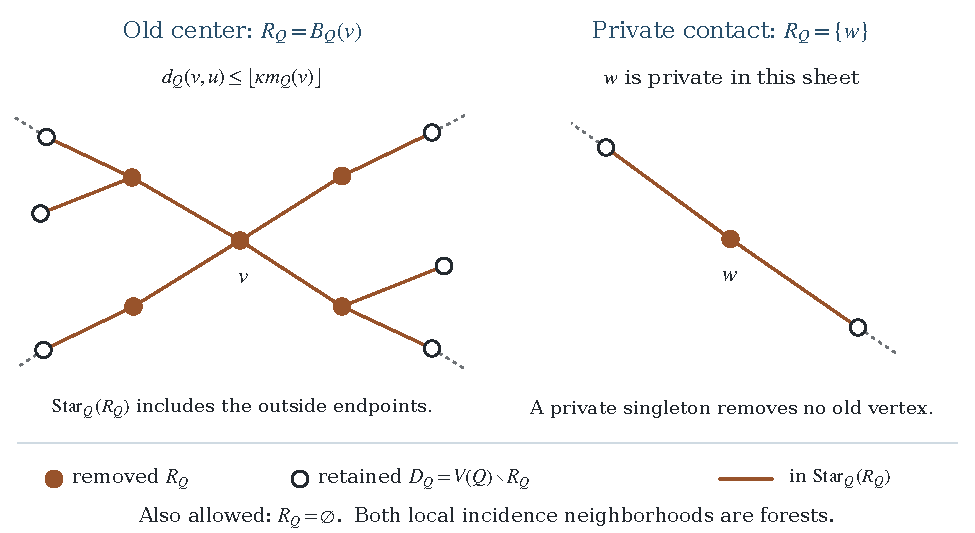
\includegraphics[width=\linewidth]{figures/allowed-domains.pdf}
  \caption{Schematic incidence neighborhoods of allowed removed sets:
  an old-centered ball or a private singleton of degree two. Filled
  vertices lie in $R_Q$; hollow vertices remain in $D_Q$.
  Colored edges have an endpoint in $R_Q$, so their outside endpoints
  also belong to $\operatorname{Star}_Q(R_Q)$. These neighborhoods are
  forests by Lemma~\ref{lem:allowed-domain-sets}. Dashed continuations
  represent unspecified sheet paths. Graph-metric lengths and
  cardinalities are not drawn to scale.}
  \label{fig:allowed-domains}
\end{figure}

For a finite family $\mathcal F\subseteq\mathcal Q$, the contact set of
$Q\in\mathcal F$ is
\[
 I_{\mathcal F}(Q)=V(Q)\cap
       \bigcup_{R\in\mathcal F\setminus\{Q\}}V(R).
\]
These sets need not be finite.  In particular, the fact that comparison
arcs have no private edges does not exclude a singleton contact at a
private vertex.  The next lemma includes that case explicitly.

\begin{lemma}[Finite peeling]
\label{lem:sheet-peeling}
Every nonempty finite family $\mathcal F$ has a sheet $Q$ for which
$I_{\mathcal F}(Q)$ is either empty, contained in $B_Q(v)$ for some old
contact $v$, or equal to a singleton private contact.
Consequently the family can be ordered $Q_1,\ldots,Q_n$ with allowed
removed sets $R_j$ of those three forms such that
\begin{equation}
 V(Q_j)\cap\bigcup_{\ell>j}V(Q_\ell)\subseteq R_j.
 \label{eq:finite-peeling-overlap}
\end{equation}
\end{lemma}

\begin{proof}
Suppose that no sheet has one of the three properties.  Every sheet
then has a contact.  We will construct a polygon in distinct sheets with
all but one side forced to use either a private edge or at least four
comparison arcs.  The exterior-arc bound will exclude this polygon.

Enter a sheet at a contact $u$.  If $u$ is old,
choose a contact $w\notin B_Q(u)$; its integer distance from $u$ is
strictly greater than $\kappa m_Q(u)$.  If $u$ is private, choose any
contact $w\ne u$, which is possible because the contact set is not
that private singleton.  Transfer at $w$ to another sheet containing
it and repeat.  Since the family is finite and consecutive sheets
are different, a sheet eventually repeats.  At the first repetition,
retain the intervening $k\geq2$ distinct sheets and close the path
inside the repeated sheet.  The resulting polygon has $k-1$ chosen
nonconstant sides; only the closing side is unrestricted.

Apply Lemma~\ref{lem:sheet-polygon} with all these contact vertices
fixed.  If a chosen side has a private endpoint in its sheet, any
nonconstant path with those endpoints starts or ends with a private
 edge.  Some private edge is therefore unavoidable in every replacement
 path with the same distinct endpoints.  Yet every arc of the reduced
side is a comparison arc, none of which contains a private edge.
This is impossible.  Otherwise all $k-1$ chosen sides have old
endpoints and have intrinsic endpoint distance greater than
$\kappa m_Q(u)$ at their incoming contacts.  By
Equation~\eqref{eq:three-domain-arcs}, each such side requires at least
four exterior arc incidences.  There are therefore at least
$4(k-1)>4k-6$ exterior incidences, again a contradiction.  The argument
does not require the closing side to be nonconstant or long.

Remove the sheet just obtained and apply the same assertion to the
remaining finite family.  At each removal take its whole contact ball,
its private singleton, or the empty set, respectively.  This gives
Equation~\eqref{eq:finite-peeling-overlap}.
\end{proof}

\subsection{Finite cycle coordinates}

An oriented edge chain over a commutative ring $R$ always means a
finite-support chain.  The cycle module of a graph $Y$ is
$Z_1(Y;R)=\ker(\partial:C_1(Y;R)\to C_0(Y;R))$.  A forest has no
nonzero such cycle: the support of a proposed cycle is a finite forest,
and its coefficient at an edge incident to a leaf must vanish; repeated
leaf removal removes the whole support.

\begin{lemma}[Direct cycle coordinates]
\label{lem:sheet-cycle-coordinates}
For every commutative coefficient ring $R$, the sum of the inclusions
is an isomorphism
\begin{equation}
 \Phi_R:\bigoplus_{Q\in\mathcal Q}Z_1(Q;R)
       \longrightarrow Z_1(\mathcal C;R),\qquad
       (c_Q)_Q\longmapsto\sum_Qc_Q.
 \label{eq:sheet-cycle-isomorphism}
\end{equation}
Both the direct sum and every chain appearing here have finite support.
\end{lemma}

\begin{proof}
First, every finite cycle chain in a graph is a finite linear
combination of circuit chains.  To see this, take a spanning forest
of its finite support graph.  For each edge outside that forest,
subtract its coefficient times the circuit formed with the forest
path between its endpoints.  This removes all edges outside the
forest.  The remainder is a cycle supported on a forest and is zero.
Loops and pairs of parallel edges are included in this argument.

Let a circuit in $\mathcal C$ start at $g$ and read the word $w$.
The definition of $\Gamma$ means that, in the free group on the
formal labels, $w$ is a finite product of conjugates of words read on
closed walks of $\widetilde X$, and their inverses.  Follow that
product from $g$ in $\mathcal C$.  Each conjugating stem is traversed
once in each direction, so its oriented chain cancels.  Each relator
walk lies in a translated sheet.  Free cancellation of adjacent
inverse letters also cancels the corresponding oriented edge chains
in the formal Cayley graph.  Thus the circuit chain is a finite sum
of sheet cycle chains.  The preceding circuit decomposition proves
surjectivity of $\Phi_R$.

For injectivity, suppose that $\sum_{j=1}^n c_{Q_j}=0$.  Order the
finitely many sheets in this relation by Lemma~\ref{lem:sheet-peeling}.
An edge of $Q_1$ with a nonzero coefficient in $c_{Q_1}$ must occur
in another nonzero coordinate, since the total coefficient is zero.
Both endpoints of that edge are contacts with a later sheet and
belong to $R_1$.  Hence $c_{Q_1}$ is supported on
$\operatorname{Star}_{Q_1}(R_1)$, a forest by
Lemma~\ref{lem:allowed-domain-sets}, and is zero.  Remove this
coordinate and repeat.  Every coordinate is zero.
\end{proof}

\subsection{Simultaneous domains for the analytic realization}

We now choose removed sets on all sheets at once, so that the retained
domains are disjoint and every Cayley circuit contains an edge internal to
one of them.  The cycle coordinates just proved provide finite witnesses
for this second requirement, allowing both requirements to pass to a limit.

\begin{proposition}[Simultaneous disjoint domains]
\label{prop:domains}
There are sets $R_Q\subseteq V(Q)$, one for each sheet, such that each
$R_Q$ is empty, an old-centered ball $B_Q(v)$, or a private singleton,
and the sets $D_Q=V(Q)\setminus R_Q$ have the following properties.
\begin{enumerate}
 \item The physical vertex sets $D_Q$ are pairwise disjoint.
 \item Put
 \[
 E_{\mathrm{int}}=
 \bigcup_{Q\in\mathcal Q}
 \{e\in E(Q):\text{both endpoints of }e\text{ lie in }D_Q\}.
 \]
 Every edge in this union has a unique such sheet, and
 $(V(\mathcal C),E(\mathcal C)\setminus E_{\mathrm{int}})$ is a forest.
 \item $\operatorname{Star}_Q(R_Q)$ is a forest.  If $R_Q$ contains an
 old vertex of layer $i$, then $\abs{R_Q}\leq2^{10H_i}$.  A private
 singleton removes no old coordinate.
\end{enumerate}
No equivariance of the choices $R_Q$ is asserted or needed.
\end{proposition}

\begin{proof}
We first describe the possible limits of allowed removed sets.  We then
express disjointness and the residual-forest requirement by conditions on
finitely many membership coordinates, verify them on finite families by
peeling, and take a diagonal limit.

For a fixed sheet $Q$, let $\mathcal K_Q$ be the collection of all
allowed removed sets in the statement, represented by their
characteristic functions in $\{0,1\}^{V(Q)}$.  Every fixed vertex $p$
belongs to only finitely many allowed old-centered balls.  Indeed, if
$p\in B_Q(v)$, then
\[
 d_Q(p,v)\leq\kappa m_Q(v)
 \leq\kappa\bigl(m_Q(p)+a d_Q(p,v)\bigr),
 \qquad
 d_Q(p,v)\leq\frac{\kappa m_Q(p)}{1-\kappa a}.
\]
The last radius is finite, and $Q$ is locally finite.  Also $p$
belongs to at most one allowed private singleton.  It follows that
$\mathcal K_Q$ is closed in the characteristic-function topology.
For completeness, if a pointwise limit is nonempty, choose a vertex
$p$ in it.  All sufficiently late removed sets contain $p$, so they
belong to a fixed finite collection.  A subsequence has one constant
value, which must equal the pointwise limit.  If the limit is empty,
it is an allowed value already.  This also explains why the empty
choice must be retained.

All vertices, sheets, finite circuits, and their incidences are
countable.  Choose an orientation for each finite circuit $C$ of
$\mathcal C$ and let $c_C$ be its integral circuit chain.  Using
$\Phi_{\Z}$ from Lemma~\ref{lem:sheet-cycle-coordinates}, fix its
finite decomposition
\begin{equation}
 c_C=\sum_{Q\in\mathcal F_C}c_{C,Q},
 \qquad \abs{\mathcal F_C}<\infty.
 \label{eq:fixed-circuit-decomposition}
\end{equation}
We impose the following countable
collection of finite-coordinate conditions on the removed sets:
\begin{enumerate}
 \item For each physical vertex $x$ and distinct sheets $Q,R$ containing
 it, $x$ is not retained in both $D_Q$ and $D_R$.
 \item For each circuit $C$, there are $Q\in\mathcal F_C$ and
 $e\in E(C)\cap E(Q)$ such that both endpoints of $e$ lie in $D_Q$.
\end{enumerate}
Each condition is a finite Boolean condition, hence is preserved by
coordinatewise limits.  In the second condition both the list of
edges and the list of candidate sheets are finite.  Replacing that
list by all sheets would not give the same closedness argument.

Any finite collection of these conditions can be satisfied.  Take
the finite union of all sheets appearing in the selected first-type
conditions and of all sets $\mathcal F_C$ for the selected second-type
conditions.  Peel this finite family by
Lemma~\ref{lem:sheet-peeling} and use its allowed removed sets.  Assign
the empty removed set to every sheet outside the family.  The
selected first-type conditions hold by
Equation~\eqref{eq:finite-peeling-overlap}.

Suppose that a selected circuit condition failed.  In its
decomposition~\eqref{eq:fixed-circuit-decomposition}, take the earliest
peeled sheet with a nonzero coordinate, after discarding earlier zero
coordinates.  An edge of this coordinate whose two endpoints lie
outside its removed set cannot occur in any later coordinate: if it
did, its endpoints would be contacts in the removed set.  If this
edge belonged to $C$, it and the present sheet would witness the
selected condition, contrary to its failure.  Hence it lies outside
$C$, and its coefficient in $c_C$, and therefore in the present
coordinate, is zero.  Thus the coordinate is supported on the incidence
neighborhood of its removed set and is a cycle in a forest.  It is
zero.  Induction removes all its coordinates, contradicting
$c_C\ne0$.  This proves finite satisfiability.

Here one can finish by an explicit diagonal argument.  Enumerate
all the conditions, and for each $n$ choose a full assignment
satisfying the first $n$.  Enumerate the countably many membership
coordinates $(Q,v)$.  Pass successively to an infinite subsequence
on which the first coordinate is constant, one on which the second
is constant, and so on, and take the diagonal subsequence.  It
converges pointwise.  The preceding closedness argument shows that
each sheet's limiting removed set belongs to $\mathcal K_Q$.  Every
one of the finitely supported conditions holds in the limit.

The first conditions give disjoint domains.  An edge internal to
two domains would have an endpoint in their intersection, so its
sheet is unique.  A circuit in the residual graph would violate its
own second-type condition.  The residual graph is therefore a
forest.  The last assertions follow from
Lemma~\ref{lem:allowed-domain-sets}.
\end{proof}

\begin{lemma}[Incidence coordinates]
\label{lem:sheet-incidences}
The map sending a sheet incidence to its physical vertex and its
base type is a bijection
\begin{equation}
 \{(Q,u):Q\in\mathcal Q,\ u\in V(Q)\}
       \longrightarrow \Gamma\times V(X).
 \label{eq:sheet-incidence-bijection}
\end{equation}
In particular, a physical vertex occurs in at most
$n_i^{\mathrm{full}}=\abs{\mathscr A_i}+\abs{\mathscr B_i}$ old layer-$i$ incidences,
and
\begin{equation}
 n_i^{\mathrm{full}}=(1+2^{2r-s})2^{H_i}\leq C_s2^{H_i}.
 \label{eq:old-layer-incidences}
\end{equation}
\end{lemma}

\begin{proof}
Normalize the embedded reference sheet as
$j(v,f)=f t_v$, with $f\in\HH$ and $v\in V(X)$.  The deck group is
identified with its embedded image in $\Gamma$.  A sheet is $hQ_0$
for a coset $h\HH$, because its stabilizer is $\HH$.
At a physical vertex $u$ and specified base type $v$, the equality
$u=hf t_v$ forces and is achieved by the unique coset
$h\HH=u t_v^{-1}\HH$.  Embeddedness makes its source vertex unique.
This proves the bijection.  The displayed cardinality follows from
the definitions of the two old layer state sets.  It counts only old
types; private singleton removals add no old incidence or active old
coordinate.
\end{proof}

\subsection{The cone complex and exact chains}

The cone-chain and prime-order obstruction method follows
\cite[Section~7.6]{OpenAIProjection}.  We prove its exact-chain
interfaces for the present sheets below.  The integral detector
extension and Bott realization are separate arguments of this manuscript.

We return to the cycle coordinates to obtain the topological consequences.
This argument uses the full sheets and is independent of the domain
choices.  Start with
$\mathcal C$, add one vertex $c_Q$ for every $Q\in\mathcal Q$, and
add a spoke $\sigma_{Q,u}$ directed from $c_Q$ to each $u\in V(Q)$.
For every positive edge $e:u\longrightarrow v$ of $Q$, attach a
separate triangular cell $\tau_{Q,e}$ with cellular boundary
\begin{equation}
 \partial\tau_{Q,e}=e+\sigma_{Q,u}-\sigma_{Q,v}.
 \label{eq:cone-boundary}
\end{equation}
The resulting two-dimensional CW complex is denoted $\mathcal Z$.
Different sheet occurrences give different triangles and spokes,
even when their images in $\mathcal C$ agree.  This cell description
also defines the complex for infinite sheets without using any
infinite chain sums.

\begin{lemma}[Exact cone chains]
\label{lem:cone-exact}
For every commutative coefficient ring $R$, the augmented cellular
complex
\begin{equation}
 0\longrightarrow C_2(\mathcal Z;R)
 \xrightarrow{\partial_2} C_1(\mathcal Z;R)
 \xrightarrow{\partial_1} C_0(\mathcal Z;R)
 \xrightarrow{\varepsilon}R\longrightarrow0
 \label{eq:exact-cone-complex}
\end{equation}
is exact.  This assertion depends on finite cycle coordinates,
not on the compactness step in Proposition~\ref{prop:domains}.
\end{lemma}

\begin{proof}
For an edge chain $b$ in a sheet $Q$, let $c_Q*b$ denote the same
linear combination of its triangles, and let $\sigma_Q(t)$ denote
the spoke chain with coefficients given by a vertex chain $t$ in
that sheet.  Equation~\eqref{eq:cone-boundary} reads
\[
 \partial(c_Q*b)=b-\sigma_Q(\partial b).
\]
Any finite $2$-chain determines a finite family of sheet edge chains
$b_Q$.  If its boundary vanishes, its components on the distinct
spoke sets give $\partial b_Q=0$ for every $Q$.  Its original-edge
component is then $\sum_Q b_Q=0$.  Injectivity of
$\Phi_R$ in Lemma~\ref{lem:sheet-cycle-coordinates} forces every
$b_Q=0$, proving injectivity at $C_2$.

Let $b+\sum_Q\sigma_Q(t_Q)$ be a finite $1$-cycle, with $b$ on
$\mathcal C$.  Its coefficient at $c_Q$ says
$\varepsilon(t_Q)=0$.  Since $Q$ is connected, $t_Q$ is the boundary
of a finite edge chain $a_Q$: join the finitely many supporting
vertices to one chosen vertex by finite paths and use their
coefficients.  Adding $\sum_Q\partial(c_Q*a_Q)$ removes all spoke
terms.  The remaining $1$-cycle lies on $\mathcal C$, and
surjectivity of $\Phi_R$ writes it as a finite sum of sheet cycles.
Each such cycle is the boundary of the identical combination of
its cone triangles.  Hence the original $1$-cycle was a boundary.

Finally $\mathcal C$ is connected and every cone is attached to it.
A finite vertex chain of total coefficient zero is the boundary of
paths to a fixed vertex.  This proves exactness at $C_0$ and at
the augmentation.  There are no cells of dimension greater than two.
Every argument involved finite-support chains only.
\end{proof}

Left translation acts cellularly on $\mathcal Z$ and preserves all
specified positive orientations.  Write $A=\Z\Gamma$ and
$B=\Z\HH$.  Its cellular modules satisfy
\begin{equation}
 C_1(\mathcal Z;\Z),\ C_2(\mathcal Z;\Z)
 \text{ are free }A\text{-modules},\qquad
 C_0(\mathcal Z;\Z)\cong A\oplus A\otimes_B\Z.
 \label{eq:cone-orbit-modules}
\end{equation}
Indeed stabilizing a formal generator edge fixes its initial group
vertex; stabilizing a spoke fixes its group-vertex endpoint; and
stabilizing a triangle fixes its specified positive base edge.
All three stabilizers are trivial.  The group vertices form one
free orbit, and the cone vertices form the orbit $\Gamma/\HH$.
These observations prove Equation~\eqref{eq:cone-orbit-modules}
without assuming torsion-freeness of $\Gamma$ and without making
the domain choices equivariant.

\subsection{The prime-order obstruction}

We record the elementary resolution comparison used both here and
in the detector argument below.  Modules and resolutions in this
paragraph may have arbitrary free ranks.

\begin{lemma}[Comparison of free resolutions]
\label{lem:free-resolution-comparison}
Let $P_\bullet\to M$ and $Q_\bullet\to N$ be exact augmented
complexes of free modules over a ring $A$.  Every homomorphism
$M\to N$ lifts to a chain map $P_\bullet\to Q_\bullet$.
Any two such lifts are chain homotopic.  In particular, two free
resolutions of one module are chain homotopy equivalent, and remain
so after tensoring with a right $A$-module or applying
$\operatorname{Hom}_A(-,L)$.
\end{lemma}

\begin{proof}
Choose the image of each free basis vector of $P_0$ to lift its
prescribed image under augmentation.  Having defined the map through
degree $n-1$, the desired image of the boundary of a basis vector
of $P_n$ is a cycle in $Q_{n-1}$.  Exactness supplies a preimage in
$Q_n$.  Choose it and extend linearly.  This constructs the chain
map in every degree.

For two lifts, let $f$ be their difference.  Its augmentation is
zero.  Inductively suppose that $h_{n-1}$ has been chosen with
the earlier homotopy identities.  The map
$f_n-h_{n-1}\partial_n$ takes values in the cycles of $Q_n$;
this follows on applying the boundary and using the chain-map
identity and the preceding homotopy identity.  Choose preimages
on the free basis of $P_n$ to obtain $h_n$.  Then
$f_n=\partial_{n+1}h_n+h_{n-1}\partial_n$.
For $n=0$ the same argument uses the zero augmentation.  Thus the
lifts are homotopic.  Lifts of the identity in both directions give
the stated chain homotopy equivalence.  Tensor and Hom preserve
the displayed homotopy equations.  No step requires a finite basis.
\end{proof}

\begin{lemma}[No prime-order subgroup]
\label{lem:no-prime-torsion}
The group $\Gamma$ is torsion-free.
\end{lemma}

\begin{proof}
The integral Heisenberg group is torsion-free.  For example, in
matrix coordinates $(\alpha,\beta,\gamma)\in\Z^3$, the normal-form
element $x^n y^l z^c$ from Section~\ref{sec:analysis} has coordinates
$(\alpha,\beta,\gamma)=(n,l,c+nl)$.  Its law is
\begin{equation}
 (\alpha,\beta,\gamma)(\alpha',\beta',\gamma')
 = (\alpha+\alpha',\beta+\beta',
       \gamma+\gamma'+\alpha\beta').
 \label{eq:heisenberg-coordinates}
\end{equation}
If a positive power is the identity, its first two coordinates
force $\alpha=\beta=0$, and its third then forces $\gamma=0$.

Suppose $P\leq\Gamma$ has prime order $p$.  The stabilizer of a
cone vertex is a conjugate of $\HH$, so it intersects $P$
trivially.  The other cell stabilizers are already trivial by
Equation~\eqref{eq:cone-orbit-modules}.  Thus $P$ acts freely on
the set of cells of every dimension.  This is freeness of setwise
cell stabilizers, not just absence of pointwise-fixed edges.  In
particular, no involution can invert a formal positive Cayley edge.
Choosing orbit representatives gives free modules over
$A_p=\F_p[P]$.  Lemma~\ref{lem:cone-exact}, with coefficients
$\F_p$, would give a free resolution of its trivial module of
length two.

Let $t=u-1$ for a generator $u$ of $P$.  Then
$A_p\cong\F_p[t]/(t^p)$, and the complex
\begin{equation}
 \cdots\xrightarrow{t}A_p\xrightarrow{t^{p-1}}A_p
 \xrightarrow{t}A_p\xrightarrow{t^{p-1}}A_p
 \xrightarrow{t}A_p\longrightarrow\F_p\longrightarrow0
 \label{eq:cyclic-periodic-resolution}
\end{equation}
is exact.  In the basis $1,t,\ldots,t^{p-1}$, the kernels of
multiplication by $t$ and $t^{p-1}$ are respectively
$(t^{p-1})$ and $(t)$.  Tensoring this resolution with the trivial
right module $\F_p$ makes every differential zero; its homology
is $\F_p$ in every nonnegative degree.  Tensoring the alleged
length-two resolution gives zero homology in every degree above
two.  This contradicts Lemma~\ref{lem:free-resolution-comparison}.
Hence $\Gamma$ has no subgroup of prime order.  A nonidentity
element of finite order $n$ would have a power of order $p$ for
any prime divisor $p$ of $n$, which proves the assertion.
\end{proof}

\subsection{The primitive class on the Heisenberg torus}

We first construct an integral class on $\HH$ that evaluates to $-1$ on
the ordered torus $(z,x)$, and then prove that it extends to $\Gamma$.
We use an explicit bar model both to compute this evaluation and to
identify the extension map with pullback on classifying spaces.
For a group $\Lambda$, let $\mathcal B_n(\Lambda)$ be
the free abelian group on ordered tuples
$(g_0,\ldots,g_n)\in\Lambda^{n+1}$, with diagonal left action,
alternating deletion boundary, and augmentation one on every
vertex.  It is free over $\Z\Lambda$: each orbit has a unique
representative with $g_0=1$.  Prepending $1$ gives an abelian-group
contracting homotopy, since direct cancellation in the deletion
formula gives $\partial s+s\partial=\id$, including the
augmentation.  Thus $\mathcal B_\bullet(\Lambda)$ is a free
resolution of the trivial module.

The realization of the semi-simplicial set of these ordered tuples
is a contractible free $\Lambda$--CW complex.  On the simplex
$(g_0,\ldots,g_n)$ with barycentric coordinates $(t_0,\ldots,t_n)$,
the contraction has value in $(1,g_0,\ldots,g_n)$ with coordinates
$(u,(1-u)t_0,\ldots,(1-u)t_n)$, for $0\leq u\leq1$.
These formulas agree under deletion of zero-coordinate faces.
The quotient has one vertex, loops $[g]$, and triangular relations
$[g][h]=[gh]$, so its fundamental group is $\Lambda$.  Lifting a
simplex from an initial vertex $g_0$ produces the tuple
$(g_0,g_0g_1,g_0g_1g_2,\ldots,g_0g_1\cdots g_n)$; its face rules
are precisely the preceding deletion rules.  Thus the contractible
tuple complex is its universal cover, and the quotient is a model
for $B\Lambda$.  Its integral cellular cochain complex is
$\operatorname{Hom}_{\Z\Lambda}(\mathcal B_\bullet(\Lambda),\Z)$.
Consequently its cohomology is $H^*(B\Lambda;\Z)$, or equivalently
$\operatorname{Ext}^*_{\Z\Lambda}(\Z,\Z)$ computed with this
resolution.  A subgroup inclusion induces the inclusion of the
tuple complexes, so restriction of these cochains is precisely
pullback on the indicated classifying spaces.

We write $[g_1\mid\cdots\mid g_n]$ for the orbit representative
$(1,g_1,g_1g_2,\ldots,g_1\cdots g_n)$.  In particular,
\[
 \partial[g\mid h]=g[h]-[gh]+[g],\qquad
 \partial[g\mid h\mid k]
 =g[h\mid k]-[gh\mid k]+[g\mid hk]-[g\mid h].
\]
With trivial coefficients these are the inhomogeneous group
cochain formulas used below.

\begin{lemma}[A primitive Heisenberg detector]
\label{lem:explicit-heisenberg-detector}
In the coordinates of Equation~\eqref{eq:heisenberg-coordinates},
the integer function
\begin{equation}
 \omega\bigl((\alpha,\beta,\gamma),
              (\alpha',\beta',\gamma')\bigr)
    =\alpha\gamma'+\binom{\alpha}{2}\beta'
 \label{eq:explicit-heisenberg-cocycle}
\end{equation}
is a normalized group $2$-cocycle.  Its class $c_{\HH}$ evaluates
to $-1$ on the torus with ordered generators $(z,x)$.
\end{lemma}

\begin{proof}
The binomial expression $\binom{\alpha}{2}=\alpha(\alpha-1)/2$
is an integer also for negative $\alpha$.  Normalization follows
immediately from Equation~\eqref{eq:explicit-heisenberg-cocycle}.
Using Equation~\eqref{eq:heisenberg-coordinates}, the identity
\[
 \binom{\alpha+\alpha'}{2}
 =\binom{\alpha}{2}+\binom{\alpha'}{2}+\alpha\alpha'
\]
gives, for all $g,h,k\in\HH$,
\[
 \omega(g,h)+\omega(gh,k)
       =\omega(h,k)+\omega(g,hk).
\]
Explicitly, the only mixed term added to the central coordinate
of $hk$ is $\alpha'\beta''$; multiplying it by $\alpha$ agrees
with the mixed term $\alpha\alpha'\beta''$ in the binomial
identity.  All other terms on the two sides coincide separately.
This proves the cocycle equation in the inhomogeneous bar complex.
Equivalently, the multiplication
\[
 (t,g)(t',h)=(t+t'+\omega(g,h),gh)
\]
on $\Z\times\HH$ is associative, with central kernel
$\Z\times\{1\}$, and defines the corresponding integral
central extension.  For the canonical lifts
$X=(0,x)$, $Y=(0,y)$, $Z=(0,z)$ and the positive central
kernel generator $T=(1,1)$, one has
$[X,Y]=Z$, $[X,Z]=T$, and $Y,Z,T$ commute.  This is the
unipotent shear extension that lengthens the Heisenberg block.

The subgroup generated by
$z=(0,0,1)$ and $x=(1,0,0)$ is freely abelian of rank two:
$z^u x^v=(v,0,u)$ in these coordinates.  For its oriented torus,
the bar $2$-chain
\[
 [z\mid x]-[x\mid z]
\]
represents the oriented fundamental class.  To check the sign and
the normalization directly, subdivide the fundamental square with
successive vertices $1,z,zx,x$ by the diagonal from $1$ to $zx$.
The two oriented triangles give $(1,z,zx)-(1,x,xz)$, which are
the displayed inhomogeneous bar chains.  Sending grid vertices
$(u,v)$ to $z^u x^v$ supplies the equivariant map from the
triangulated universal cover of the torus into the bar model.
Evaluation is therefore
\[
 \omega(z,x)-\omega(x,z)=0-1=-1.
\]
\end{proof}

\subsection{Extending integral degree-two classes}

The class $c_{\HH}$ now gives the detector on the embedded torus.
It remains to extend it from $\HH$ to $\Gamma$.  The exact cone chains
prove the stronger assertion that every integral degree-two class on
$\HH$ extends.

\begin{lemma}[Integral restriction is onto in degree two]
\label{lem:degree-two-restriction}
The inclusion of the deck subgroup induces a surjection
\begin{equation}
 H^2(B\Gamma;\Z)\longrightarrow H^2(B\HH;\Z).
 \label{eq:degree-two-restriction}
\end{equation}
\end{lemma}

\begin{proof}
Put $A=\Z\Gamma$, $B=\Z\HH$, $M=\Z$, and
$C_0=C_0(\mathcal Z;\Z)$.  By
Lemma~\ref{lem:cone-exact} and
Equation~\eqref{eq:cone-orbit-modules}, the module
$K=\ker(C_0\to M)$ has a length-one free resolution
\[
 0\longrightarrow P_1=C_2(\mathcal Z;\Z)
 \xrightarrow{d_P}P_0=C_1(\mathcal Z;\Z)
 \longrightarrow K\longrightarrow0.
\]
This is the vanishing of
$\operatorname{Ext}^2_A(K,M)$ that makes the degree-two restriction
map surjective.  The proof has two parts: we construct the resulting
surjection in Ext using a free resolution, and then identify it with
restriction by comparing the induced Heisenberg resolution with the bar
resolution of $\Gamma$.

As a right $B$-module, $A$ is a direct sum of copies of $B$, using
representatives of the cosets $\Gamma/\HH$.  Therefore
\[
 I_\bullet=A\otimes_B\mathcal B_\bullet(\HH)
\]
is an exact free $A$-resolution of $A\otimes_B M$.
Let $Q_\bullet$ resolve $C_0=A\oplus A\otimes_B M$ by taking
$Q_0=A\oplus I_0$, $Q_n=I_n$ for $n\geq1$, with the extra $A$
summand concentrated in degree zero.  Lift $K\hookrightarrow C_0$
to a chain map $f:P_\bullet\to Q_\bullet$ as follows.
Choose $f_0$ on a free basis to lift that inclusion.  The elements
$f_0d_P(P_1)$ have zero augmentation in $C_0$, so exactness of
$Q_\bullet$ permits a lift $f_1:P_1\to Q_1$ with
$d_Qf_1=f_0d_P$.  There are no higher $P$ terms.

Define a free augmented complex $T_\bullet\to M$ by
\[
 T_0=Q_0,\qquad T_n=Q_n\oplus P_{n-1}\quad(n\geq1),
\]
where $P_j=0$ for $j\geq2$, with boundary
\[
 d_T(q,p)=(d_Qq+f_{n-1}p,-d_Pp)\quad(n\geq2),\qquad
 d_T(q,p)=d_Qq+f_0p\quad(n=1).
\]
The augmentation is $Q_0\to C_0\to M$.
The identities defining $f$ give $d_T^2=0$.
This complex is exact.  In degree two, a cycle $(q,p)$ has
$d_Pp=0$, hence $p=0$, and then $q$ bounds in $Q_\bullet$.
The same is immediate in degrees at least three.  In degree one,
if $d_Qq+f_0p=0$, augmentation in $C_0$ implies that $p=d_Pp_1$
for some $p_1$.  Then $q+f_1p_1$ is a $Q$-cycle and equals
$d_Qq_2$; thus $(q,p)=d_T(q_2,-p_1)$.  In degree zero, an element
mapping to zero in $M$ has augmentation in $K$; subtract a suitable
$f_0p$ and then lift the remainder through $d_Q$.  Surjectivity of
the augmentation is immediate.  Hence $T_\bullet$ is a free
resolution of $M$.

The inclusion $Q_\bullet\to T_\bullet$ lifts $C_0\to M$.
Any degree-two cocycle $\phi:Q_2\to M$ extends to
$\psi:T_2=Q_2\oplus P_1\to M$ by $\psi(q,p)=\phi(q)$.
It is still a cocycle because $T_3=Q_3$ and its boundary has
zero $P_1$ component.  Therefore the induced map
\begin{equation}
 \operatorname{Ext}^2_A(M,M)
 \longrightarrow\operatorname{Ext}^2_A(C_0,M)
 \label{eq:ext-surjection}
\end{equation}
is surjective.  This is explicitly the degree-two portion of
the Ext sequence for $0\to K\to C_0\to M\to0$.

There is a cochain isomorphism
\begin{equation}
 \operatorname{Hom}_A
   (A\otimes_B\mathcal B_n(\HH),M)
 \longrightarrow
 \operatorname{Hom}_B(\mathcal B_n(\HH),M),\qquad
 \phi\longmapsto\bigl(b\mapsto\phi(1\otimes b)\bigr).
 \label{eq:explicit-shapiro}
\end{equation}
Its inverse sends $\eta$ to $a\otimes b\mapsto a\eta(b)$;
this is well-defined by $B$-linearity and is $A$-linear.
The maps commute with the boundaries.  The extra free $A$
summand in $Q_0$ contributes no cohomology in degree two, so
Equation~\eqref{eq:explicit-shapiro} identifies the target of
Equation~\eqref{eq:ext-surjection} with $H^2(B\HH;\Z)$.
This proves the needed instance of Shapiro's isomorphism at
the cochain level.

It remains to identify the map, rather than just its two groups.
Let $\mathcal B_\bullet(\Gamma)$ be the preceding bar resolution.
Choose a comparison map $T_\bullet\to\mathcal B_\bullet(\Gamma)$
lifting the identity of $M$.  The composite
\[
 I_\bullet\longrightarrow Q_\bullet\longrightarrow T_\bullet
 \longrightarrow\mathcal B_\bullet(\Gamma)
\]
lifts the augmentation $A\otimes_B M\to M$.  Another such lift
is the explicit map
\[
 \theta\bigl(a\otimes(h_0,\ldots,h_n)\bigr)
       =a\,(h_0,\ldots,h_n),
\]
where the tuple on the right is viewed in $\Gamma$.
Lemma~\ref{lem:free-resolution-comparison} makes these lifts
chain homotopic.  After Equation~\eqref{eq:explicit-shapiro},
precomposition with $\theta$ restricts a $\Gamma$-cochain to
tuples from $\HH$.  As observed in the bar model, this is exactly
pullback along $B\HH\to B\Gamma$.  Thus the surjection in
Equation~\eqref{eq:ext-surjection} is the map in
Equation~\eqref{eq:degree-two-restriction}.
\end{proof}

\begin{proposition}[Torsion-freeness and the integral detector]
\label{prop:torsion-detector}
The graphical group $\Gamma$ is torsion-free.  The map
$i_\Gamma:\Z^2\to\Gamma$ sending the ordered basis to $(z,x)$
is injective, and there is a class $c_\Gamma\in H^2(B\Gamma;\Z)$
such that
\begin{equation}
 \bigl\langle(Bi_\Gamma)^*c_\Gamma,[T^2]\bigr\rangle=-1.
 \label{eq:graphical-integral-detector}
\end{equation}
\end{proposition}

\begin{proof}
Lemma~\ref{lem:no-prime-torsion} proves torsion-freeness.
The deck embedding of Proposition~\ref{prop:graphical-realization}
and the coordinate calculation in
Lemma~\ref{lem:explicit-heisenberg-detector} prove injectivity of
$i_\Gamma$.  Choose $c_\Gamma$ mapping to $c_{\HH}$ under the
surjection of Lemma~\ref{lem:degree-two-restriction}.  Its map
was identified there with actual restriction in integral
cohomology.  Equation~\eqref{eq:graphical-integral-detector}
now follows from the explicit evaluation in
Lemma~\ref{lem:explicit-heisenberg-detector}.
\end{proof}

\section{Realization of the Bott cancellation in the reduced algebra}
\label{sec:assembly}

We now prove that the rank-zero Bott class of the embedded torus
$\langle z,x\rangle$ vanishes in the reduced group algebras along a tail
of the compatible accuracy sequence constructed below.  The localized Bott
profiles from Section~\ref{sec:analysis} can be moved between neighboring heights.
We realize two families of these moves by finite Cayley formulas, using
the disjoint domains of Proposition~\ref{prop:domains}.  As the errors
tend to zero, the formulas give exact projection homotopies in a norm
sequence quotient.  Their cancellation removes the initial-height
profile.  We then identify that profile with the physical torus Bott
class and recover an exact finite witness in a single reduced group
algebra, before passing to a finitely generated subgroup.

We use the right Cayley graph and the conventions of
Proposition~\ref{prop:graphical-realization}.  Thus a positive formal edge is
$g\longrightarrow g\sigma$, the deck group acts on the left, and, after
choosing one lift of each base vertex $v$, the embedded cover has coordinates
\begin{equation}\label{eq:assembly-cover-coordinates}
 j(v,f)=f t_v\qquad(f\in\HH).
\end{equation}
We identify $\HH$ with its embedded image in $\Gamma$.  Its distinct sheets
are the left translates $h\widetilde X$, indexed by the cosets $h\HH$.
On $\ell^2(\Gamma)$ put
\[
 R(g)\delta_h=\delta_{hg^{-1}}.
\]
This is the right regular representation with the convention that
$R(g)R(k)=R(gk)$.  The unitary $I\delta_h=\delta_{h^{-1}}$ satisfies
\begin{equation}\label{eq:right-left-regular}
 I R(g) I=\lambda(g).
\end{equation}
Consequently the norm closure of the right regular group algebra is a copy
of $\Cr(\Gamma)$.  We use it throughout the estimates and apply
\eqref{eq:right-left-regular} at the end.  This equivalence sends the represented
group element $g$ to the same element $g$, so it does not introduce an
antihomomorphism on group $K$-theory.
We orient each positive old incidence edge from its $\mathscr A$ endpoint
$v$ to its $\mathscr B$ endpoint $w$.  If its label is $\sigma$ and its
forward voltage is $h_e$, then
\begin{equation}\label{eq:assembly-edge-direction}
 t_v\sigma=h_e t_w,
 \qquad
 R(\sigma)\delta_{f t_w}=\delta_{f h_e^{-1}t_v}.
\end{equation}
Thus the $\mathscr B$-to-$\mathscr A$ incidence block of $R(\sigma)$ is
the deck operator $R_{\HH}(h_e)$.  For our chosen direction a sampled
term $R_{\HH}(v_e)$ is implemented by the forward voltage $h_e=v_e$.
The opposite, forward transition operator has the adjoint convention.

We will take a sequence of constructions, indexed by $\nu$.  The integer $b$
is fixed once, including across this sequence.  The parameters $s=s_\nu$ and
$H_0=H_{0,\nu}$ may increase; the degree is fixed at all heights of any one
construction.  All matrix sizes in the Bott representatives below are fixed.
The number of incidence types, the finite weight net, and the lengths of
operator products may depend on $\nu$; these choices precede the choice of
$s_\nu$.

\subsection{Compact Bott profiles and common carriers}

Use throughout the compact Bott projection $p$ in
Equation~\eqref{eq:compact-bott-profile}, with $m=2$,
$e=e_\infty=\operatorname{diag}(0,1)$, and $a=p-e$.
The explicit eigenvectors and winding calculation in
Section~\ref{sec:analysis} prove that $[p]-[e]$ is a compactly supported
Bott generator.  This projection and its signed class are fixed for the
entire accuracy sequence.

In angular torus coordinates $(\zeta,\xi)\in(\R/\Z)^2$ corresponding to
$(z,x)$, put
\[
 Z_i=2^{500H_i},\qquad N_i^{\mathrm{freq}}=2^{200H_i},\qquad J_i=2^{50H_i},
 \qquad
 a_i(\zeta,\xi)=a\bigl(Z_i(\zeta-\alpha),N_i^{\mathrm{freq}}\xi\bigr).
\]
The functions are defined in a small coordinate chart and extended by zero;
their supports lie strictly inside that chart.  Thus $e+a_i$ is a smooth
projection on the torus.  It has the same first Chern number as $p$, so
\begin{equation}\label{eq:physical-bott-profile}
 [e+a_i]-[e]=\beta\quad\hbox{in }K_0(C(\mathbb T^2)),
\end{equation}
where $\beta$ is the torus realization of this fixed rank-zero Bott
generator.  The positive rescalings preserve its sign.

The rescaling path
\begin{equation}\label{eq:adjacent-rescaling}
 a_{i,t}(\zeta,\xi)
 =a\bigl(2^{500bt}Z_i(\zeta-\alpha),
          2^{200bt}N_i^{\mathrm{freq}}\xi\bigr),\qquad 0\le t\le1,
\end{equation}
joins $a_i$ to $a_{i+1}$.  Each $e+a_{i,t}$ is a projection.  In the rescaled
coordinates all these functions form one compact smooth family.  In
particular there is a common modulus of norm continuity in $t$, independent
of $i$ and $\nu$, because $b$ is fixed.

Choose real continuous smooth cutoffs $\chi_i$, with $0\le\chi_i\le1$,
equal to one on the supports of all profiles used at level $i$, including the
profiles $a_{i-1,t}$ transported from the preceding level.  Their supports
are contained in fixed enlargements, depending only on $b$, of the rectangle
at level $i$.  Choose an additional slightly larger Borel rectangle projection
$e_i^{\mathrm{car}}$ containing $\supp\chi_i$.  We use the same choices on
both sides of a layer.  They may be chosen so that every function used in a
block $(i,k)$, $|i-k|\le1$, is supported where both $\chi_i$ and $\chi_k$
equal one.  Indeed the largest required support at level $i$ is contained in
the rectangle of level $i-1$, and the ratios between successive widths are
the fixed numbers $2^{500b}$ and $2^{200b}$.  At $i=0$ the notation $i-1$
merely prescribes a fixed enlargement, not an additional graph layer.

Apply Proposition~\ref{prop:sampled-symbols} with these fixed enlargements.
The spread operators from Lemma~\ref{lem:supported-spreading}, written
in the right regular representation, have the form
\[
 T_i=\sum_j a_{ij}R(y)^j,
 \qquad \sum_j|a_{ij}|^2=1,
 \qquad e_i^{\mathrm{car}}T_i^*T_i e_i^{\mathrm{car}}
       =e_i^{\mathrm{car}}.
\]
Their range carriers
\begin{equation}\label{eq:spread-carrier}
 P_i=T_i e_i^{\mathrm{car}}T_i^*
\end{equation}
are projections in the containing von Neumann algebra and satisfy
\begin{equation}\label{eq:carrier-trace}
 \tau_{\HH}(P_i)=\tau_{\HH}(e_i^{\mathrm{car}})
       \le C_{\nu}2^{-700H_i}.
\end{equation}
The constant is uniform in the height.  Increasing the starting height
ensures the disjointness of the translates even for the specified enlarged
rectangles.  These Borel carriers are used only for Hilbert-space estimates.
Actual group-algebra formulas below use continuous functions and the finite
sums $T_i$; no Borel carrier is asserted to belong to a reduced $C^*$-algebra.

For one construction put $\mathscr L=\ell^2(\Gamma)$ and regard
$e_i^{\mathrm{car}}$ as a projection on $\mathscr L$ through the subgroup's
right regular operators.  The model space is
\begin{equation}\label{eq:exact-model-space}
 \mathscr K=\bigoplus_{i\ge0}e_i^{\mathrm{car}}\mathscr L.
\end{equation}
A band profile $f=(f_{ik})_{|i-k|\le1}$ from our fixed compact profile
families acts on this space from the $k$th to the $i$th summand by its
torus function $f_{ik}$.  Support in both carriers makes each block
well defined; the uniform block norm and width one give a bounded
operator $f^{\mathrm{mod}}$.
All cosets of $\HH$ carry the same profile.

The profiles we must realize have the four diagonal height patterns
\[
 \begin{array}{c|ccccc}
  &0&1&2&3&\cdots\\ \hline
  \mathrm{ev}&a_0&0&a_2&0&\cdots\\
  \mathrm{od}&0&a_1&0&a_3&\cdots\\
  \mathrm{ev},+&0&0&a_2&0&\cdots\\
  0&a_0&0&0&0&\cdots
 \end{array}
\]
Each entry is a compactly supported difference from the common scalar
projection $e$; a zero entry retains that scalar part in the full projection.  Rotating
between the disjoint pairs $(0,1),(2,3),\ldots$ and then applying
\eqref{eq:adjacent-rescaling} moves the even pattern to the odd pattern.
The pairs $(1,2),(3,4),\ldots$ similarly move the odd pattern to the
positive-even pattern.  The even pattern also splits into the
initial-height and positive-even patterns.  Our analytic task is to
realize these four profiles and the two paths in one fixed matrix size.
The estimates below first pass from this model to normalized constants
on the sheets, and then from the sheets to finite Cayley formulas.

\subsection{Domains, trimming, and bounded maps}

For this subsection fix one construction.  Let
\[
 \mathscr H_{\mathrm{abs}}=\bigoplus_Q\ell^2(Q)
\]
be the abstract orthogonal sum over its sheets.  A fixed finite matrix factor
can be tensored onto every space without changing the argument.  On each
old vertex of height $i$ use the carrier $P_i$ of
\eqref{eq:spread-carrier}.  More precisely, using the regular deck coordinate
on the lifted vertex set, let $E_{Q,i}$ be the sum of these carriers over the
old base vertices on both sides of height $i$ in sheet $Q$.  Put
\[
 E_i=\bigoplus_Q E_{Q,i},\qquad E=\bigoplus_{i\ge0}E_i.
\]
All these projections are zero on private-vertex coordinates.

Let $D_Q$ be the domains from Proposition~\ref{prop:domains}, and let $D$ be
coordinate restriction to their abstract sum.  Their physical images are
pairwise vertex-disjoint.  Thus coordinate inclusion defines a partial
isometry
\[
 U\colon\mathscr H_{\mathrm{abs}}\longrightarrow\ell^2(\Gamma),
 \qquad U^*U=D,
\]
which is an isometry on $D\mathscr H_{\mathrm{abs}}$ and is zero on its
orthogonal complement.

\begin{lemma}[Uniform trimming estimate]\label{lem:assembly-trimming}
For a construction whose constants have already been fixed,
\[
 \|(1-D_Q)E_{Q,i}\|^2\le C_\nu2^{-690H_i},
 \qquad
 \delta_\nu:=\|(1-D)E\|\le C_\nu2^{-345H_0}.
\]
In particular $H_{0,\nu}$ can be chosen so that $\delta_\nu\to0$.
If $A=EAE$ and $B=EBE$, and
\[
 \Psi_\nu(A)=UDADU^*,
\]
then
\begin{equation}\label{eq:domain-product-error}
 \|\Psi_\nu(A)\Psi_\nu(B)-\Psi_\nu(AB)\|
       \le\delta_\nu^2\|A\|\|B\|.
\end{equation}
\end{lemma}

\begin{proof}
For a projection $P$ and a finite coordinate set $B_0$, the ordinary
Hilbert--Schmidt norm gives
\[
 \|1_{B_0}P\|^2\le\|1_{B_0}P\|_{\mathrm{HS}}^2
       =\sum_{u\in B_0}\langle P\delta_u,\delta_u\rangle.
\]
In a matrix amplification one sums over the fixed matrix basis as well.
Every regular deck translate of a given old vertex has the same diagonal
trace.  If the removed set in $Q$ is an old-centered ball, then
Proposition~\ref{prop:domains} bounds its entire cardinality by $2^{10H_i}$
whenever it meets height $i$.  Equation~\eqref{eq:carrier-trace} therefore
gives the first estimate, with all repeated deck lifts counted separately.
An empty removed set costs nothing.  A private singleton also costs nothing,
since $E_{Q,i}$ has zero private coordinates.  This statement is about indexed
sheet coordinates even if the same physical vertex is old in another sheet.

Both $D$ and $E$ preserve the height decomposition.  The norm of their
orthogonal direct sum is the supremum of the block norms, which gives the
bound on $\delta_\nu$.  Finally, using $U^*U=D$, the difference in
\eqref{eq:domain-product-error} is $UD A(D-1)B D U^*$.  Its norm is at most
$\|A\|\|B\|\,\|E(1-D)E\|$, and
$\|E(1-D)E\|=\|(1-D)E\|^2$.
\end{proof}

Trimming gives the almost multiplicative map needed for all model
profiles.  To compare the initial-height profile with the physical torus
class, we also need to sum its normalized constants over sheets.  Let
$\mathcal J$ initially sum finitely supported vectors from finitely many
abstract sheets into their physical vertex coordinates.  This notation does
not presume that untrimmed summation is bounded.

\begin{lemma}[Synthesis on the active carriers]\label{lem:assembly-synthesis}
Let $n_i$ be the number of surviving old base vertices on both sides of height
$i$.  Then
\begin{equation}\label{eq:raw-synthesis-level}
 \|\mathcal J(1-D)E_i\|^2
 \le n_i\sup_Q\|(1-D_Q)E_{Q,i}\|^2
 \le C_\nu2^{-689H_i}.
\end{equation}
Consequently $\mathcal J E$ extends to a bounded operator and
\begin{equation}\label{eq:raw-synthesis-sum}
 \|\mathcal J E-UDE\|
 \le C_\nu\sum_{i\ge0}2^{-344.5H_i}
 =C_\nu\frac{2^{-344.5H_0}}{1-2^{-344.5b}}.
\end{equation}
\end{lemma}

\begin{proof}
For a physical vertex $u$ and a specified old base vertex $v$, the only sheet
coset that can contain $u$ at base type $v$ is
$u t_v^{-1}\HH$, by \eqref{eq:assembly-cover-coordinates}.  This also follows
from the incidence bijection in Lemma~\ref{lem:sheet-incidences}.  Thus at
height $i$ each physical vertex receives at most $n_i$ indexed coordinates.
Pointwise Cauchy--Schwarz gives the first inequality in
\eqref{eq:raw-synthesis-level}, initially on the stated dense domain.
The layer cardinalities give
$n_i\le C_s2^{H_i}$; Lemma~\ref{lem:assembly-trimming} gives the second
inequality.  The bounded extensions at individual heights may be summed in
operator norm, because $H_i=H_0+bi$ and the square-root estimates are
summable.  On their common dense domain
$\mathcal J E=UDE+\mathcal J(1-D)E$, proving
\eqref{eq:raw-synthesis-sum} and the claimed extension.
\end{proof}

\subsection{Finite Cayley formulas and extraction of constants}

The incidences supplied by Propositions~\ref{prop:tower-labels},
\ref{prop:sequential-law}, and~\ref{prop:pruning} will be denoted by
$U_{ik}^0\colon\ell^2(\mathscr B_k)\to
\ell^2(\mathscr A_i)$ for a pre-deletion normalized incidence,
$|i-k|\le1$, suppressing its finite type index.  It sends the normalized
constant vector to the normalized
constant vector, its adjoint does the same, and its centered norm is at most
the fixed $\rho<1$.  Let $U_{ik}$ be its compression to the surviving vertex
sets.  The deletion fraction is at most $\varepsilon_{\mathrm{del}}$ in
each side and layer.  We always normalize constant vectors using the actual
surviving vertex counts.

\begin{lemma}[Deleting a small fraction of vertices]\label{lem:deleted-incidence}
There are contractions $\widehat U_{ik}$ on the surviving spaces that send
normalized constants exactly to normalized constants in both directions,
have centered norm at most $\rho$, and satisfy
\[
 \|U_{ik}-\widehat U_{ik}\|\le C\sqrt{\varepsilon_{\mathrm{del}}}.
\]
The constant is uniform in the height and the incidence type.
\end{lemma}

\begin{proof}
For one incidence let $a,b$ be the old normalized constants and let $P_A,P_B$
be the surviving coordinate projections.  Their normalized restrictions
$a',b'$ differ from $a,b$, after extension by zero, by at most
$C\sqrt{\varepsilon_{\mathrm{del}}}$.  Put
$Q_A=1-|a'\rangle\langle a'|$ and
$Q_B=1-|b'\rangle\langle b'|$ on the surviving spaces and define
\[
 \widehat U=|a'\rangle\langle b'|+Q_AUQ_B.
\]
Write $U^0=|a\rangle\langle b|+U_0$.  Then
$Q_AP_Aa=0$ and $Q_BP_Bb=0$, so $\|Q_AUQ_B\|\le\|U_0\|\le\rho$.
The two displayed summands of $\widehat U$ have orthogonal source and range
spaces, proving its asserted gap and norm.  The estimates
$\|Ub'-a'\|+\|U^*a'-b'\|\le C\sqrt{\varepsilon_{\mathrm{del}}}$
bound the remaining three blocks in $U-\widehat U$.
\end{proof}

We embed the model space \eqref{eq:exact-model-space} using normalized
constants on the surviving $\mathscr B_i$ vertices.  The subgroup operators
preserve $\mathscr L=\bigoplus_{h\HH}\ell^2(h\HH)$.  For each coset and
height, map its vector to the corresponding sheet's normalized constant
array, applying $T_i$ to its deck coordinate.  This defines an isometry
\[
 \mathcal I\colon\mathscr K\longrightarrow\mathscr H_{\mathrm{abs}},
 \qquad \mathcal I\mathcal I^*\le E.
\]
Changing the representative of $h\HH$ changes both coordinates by a left
deck translation.  The right regular functions and $T_i$ commute with that
translation, so the map is well defined.  We write $\mathscr K_\nu$ and
$\mathcal I_\nu$ when the construction index is needed.

The $\mathscr A_i$ coordinates supply finite routes between these chosen
$\mathscr B_i$ constant coordinates.  On the full abstract sheet space
consider the compactly supported mean blocks
\begin{align*}
 V_i&=U_{ii}\otimes T_i\chi_iT_i^*,\\
 W_{ik}(f)&=U_{ik}\otimes T_i f_{ik}T_k^*.
\end{align*}
Here $V_i$ maps the $\mathscr B_i$ side to the $\mathscr A_i$ side, and
$f_{ik}$ is supported where $\chi_i=\chi_k=1$.  All functions can be
matrix-valued in a fixed dimension.  Take the sums over sheets and heights,
writing $V=\bigoplus_i V_i$ and $W(f)$ for the band matrix with blocks
$W_{ik}(f)$, $|i-k|\le1$.  They are supported on $E$, and their norms are
uniformly bounded by the ordinary block Schur estimate.

For $k\ge1$ define the finite word in these operators
\begin{equation}\label{eq:constant-route}
 \mathcal R_k(f)=(V^*V)^kV^*W(f)(V^*V)^k.
\end{equation}
On the block from the $\mathscr B_j$ side to the $\mathscr B_i$ side its
incidence factor is
\[
 (U_{ii}^*U_{ii})^k U_{ii}^*U_{ij}(U_{jj}^*U_{jj})^k.
\]
The function factor is exactly $T_i f_{ij}T_j^*$: every extra cutoff is one
on $\supp f_{ij}$.  Replacing all incidences by
Lemma~\ref{lem:deleted-incidence}'s hatted incidences changes the product by
at most $C_f k\sqrt{\varepsilon_{\mathrm{del}}}$.  On constants the hatted
incidence product is exactly the map between normalized constants.
To see the suppression on the complement, let $\Pi_i$ be the projection
onto normalized constants in the surviving $\mathscr B_i$ space.  Then
\[
 \widehat U_{ii}^*\widehat U_{ii}=\Pi_i+C_i,\qquad
 \Pi_iC_i=C_i\Pi_i=0,\qquad \|C_i\|\le\rho^2.
\]
Each flanking $k$th power therefore has centered norm at most
$\rho^{2k}$.  The intervening block preserves constants and their
orthogonal complements, so the full product has centered norm at most
$C\rho^{2k}$.  A band matrix
of width one has norm at most three times the supremum of its block norms.
We have therefore proved
\begin{equation}\label{eq:constant-extraction-error}
 \|\mathcal R_k(f)-\mathcal I f^{\mathrm{mod}}\mathcal I^*\|
 \le C_f\bigl(\rho^{2k}+k\sqrt{\varepsilon_{\mathrm{del}}}\bigr).
\end{equation}
Thus the route extracts the prescribed profile on the model coordinates
and suppresses the other incidence modes.  The estimate is in the full
operator norm, including all nonconstant coordinates.

\begin{lemma}[Finite formulas for a prescribed profile family]
\label{lem:finite-profile-realization}
Fix a finite collection of band profiles $f=(f_{ik})_{|i-k|\le1}$ of the
kind above, a fixed finite matrix size, and a target error $\eta>0$.
One can choose the construction parameters so that for each such profile
there is a finite matrix group-algebra element $b_f$ satisfying
\begin{equation}\label{eq:finite-profile-realization}
 \|b_f-UD\mathcal I f^{\mathrm{mod}}\mathcal I^*DU^*\|<\eta.
\end{equation}
The estimate holds simultaneously over all heights and sheets.  Profiles
may be set to zero on any prescribed parity pattern, on all positive heights,
or on the initial height, without a height-dependent enlargement of the
alphabet.
\end{lemma}

\begin{proof}
First choose $k$ so that the gap term in
\eqref{eq:constant-extraction-error} is sufficiently small.  Include the
finitely many cutoff and symbol blocks $V$ and $W(f)$ as designated incidence
types in Proposition~\ref{prop:sampled-symbols}.  That Proposition supplies
a finite weight net.  We first compare each sampled factor with its
compressed sheet mean, and then control the products in
\eqref{eq:constant-route}.

For a type $\tau$ define the actual finite polynomial
\begin{equation}\label{eq:finite-cayley-polynomial}
 C_\tau=q^{-1}\sum_{\sigma\in\mathcal S_\tau}
       W_\sigma R(\sigma)\in M_m(R(\C[\Gamma])),
\end{equation}
where the positive augmented label $\sigma$ determines its matrix weight
$W_\sigma$.  These weights already incorporate the bounded factor
$q/q_{\tau,ik}$ in Proposition~\ref{prop:sampled-symbols}, before finite-net
rounding; the polynomial uses the single common normalizer $q^{-1}$.
The set $\mathcal S_\tau$ is finite.
On a sheet $Q$, sum the polynomial's contributions over the
prescribed source edges of type $\tau$ in $Q$.
Equation~\eqref{eq:assembly-edge-direction} identifies this source-edge
sum, on each basis vector, with the sampled
$\mathscr B$-to-$\mathscr A$ convolution for that type, with forward
voltage equal to the sampled group element.  The sampled operator
differs in full regular norm from its prescribed mean by an arbitrarily
small uniform amount.

Compressing to the disjoint domains and taking the orthogonal sum does not
increase the sampling error.  It remains to estimate the edges outside
that sum.  The physical Cayley polynomial and this domain sum
differ precisely on the remaining formal edges, with their specified
weights.  These include nonsource Cayley chords and unused weight-tag
edges, even when both endpoints lie in one retained domain.  An edge
is removed from the remainder only when it is an edge of its retained
source sheet.  Disjointness of the domains prevents any ambiguity.
The remaining edges form a forest by Proposition~\ref{prop:domains}.
A matrix adjacency on a forest of degree at most $L$ and edge weight norm
at most $w$ has norm at most $2w\sqrt L$: root each component, take the
operator sending parent coordinates to child coordinates, use that each
child has a unique parent, and add its adjoint.  For a rectangular or
directed block, self-adjoint doubling has support in the bipartite double
cover of this forest, which is again a forest.  Consequently the residual
error here is at most
\[
 C\frac{\sqrt{|\mathcal S_{\mathrm{wt}}|}}q,
\]
where $\mathcal S_{\mathrm{wt}}$ is the finite weighted old alphabet.
All private letters have coefficient zero.  Each normalized nonzero weight
has norm at most $C/q$, with $C$ fixed before $s$.  The sharp alphabet bound is
\[
 \frac{\sqrt{|\mathcal S_{\mathrm{wt}}|}}q
 \le 2^{-.000025s+O(\log s)+O_{b,\eta}(1)},
\]
which tends to zero after the finite type and net choices.  Thus every factor
of \eqref{eq:constant-route} has a finite Cayley formula close to its
$\Psi_\nu$ image in full norm.

We now use those finite formulas in the same finite word
\eqref{eq:constant-route}.  Equation~\eqref{eq:domain-product-error}
controls replacing the product of compressed means by the compression of
their product.  Ordinary telescoping controls perturbing the factors: for
a product of $r$ factors of norm at most $L$, per-factor error $\theta$
costs at most $r\theta(L+\theta)^{r-1}$.  The numbers $r,L$ are fixed before
the degree choice, so the sampling and forest errors can be chosen small
enough.  Choose $s$ and then $H_0$ also to make the deletion term and the
trimming term as small as required.  Equation~\eqref{eq:constant-extraction-error}
now proves \eqref{eq:finite-profile-realization}.

There is no physical projection selecting a height in this argument.
Instead, each designated symbol has its prescribed value, including zero,
at each block.  On a zero block Proposition~\ref{prop:sampled-symbols}
uses zero scalar weights with diffuse voltages.  The finite type and weight
tags record everything needed for the finite Cayley polynomial.  A parity
pattern or an initial-height exception changes this finite prescription but
introduces no family of new labels indexed by height.
\end{proof}

\subsection{An exact source algebra in a norm sequence quotient}

Finite-profile realization gives approximations with errors tending to zero.
We pass to norm sequence quotients to make these approximations exact.
For construction $\nu$ let $A_\nu$ be the right regular copy of
$\Cr(\Gamma_\nu)$ on $\mathscr L_\nu=\ell^2(\Gamma_\nu)$.  Define
\[
 \mathcal Q_r=\frac{\prod_\nu A_\nu}{\bigoplus_\nu A_\nu},
 \qquad
 \mathcal Q_{\mathrm{op}}
 =\frac{\prod_\nu B(\mathscr L_\nu)}{\bigoplus_\nu B(\mathscr L_\nu)}.
\]
Products mean bounded sequences and direct sums mean norm-null sequences.
The faithful coordinate representations give an isometric inclusion
$\mathcal Q_r\subset\mathcal Q_{\mathrm{op}}$.

For the model spaces in \eqref{eq:exact-model-space}, put
\[
 \mathcal M=\frac{\prod_\nu B(\mathscr K_\nu)}
                  {\bigoplus_\nu B(\mathscr K_\nu)}.
\]
Using the normalized-constant embeddings already constructed, set
\[
 V_\nu=U_\nu D_\nu\mathcal I_\nu.
\]
Lemma~\ref{lem:assembly-trimming} gives
\begin{equation}\label{eq:model-map-near-isometry}
 \|V_\nu^*V_\nu-1_{\mathscr K_\nu}\|\le\delta_\nu^2.
\end{equation}
It follows that
\begin{equation}\label{eq:model-quotient-map}
 \Theta\colon\mathcal M\longrightarrow\mathcal Q_{\mathrm{op}},
 \qquad [(b_\nu)]\longmapsto[(V_\nu b_\nu V_\nu^*)]
\end{equation}
is a $*$-homomorphism.  Indeed it is norm bounded and respects adjoints;
the multiplicative defect is at most
$\delta_\nu^2\|b_\nu\|\|c_\nu\|$.  It sends norm-null sequences to
norm-null sequences.  This establishes the exact algebraic map without
presuming that its entire image belongs to the reduced algebra quotient.

Let $A_{\mathrm{ev}},A_{\mathrm{od}},A_{\mathrm{ev},+},A_0$ denote the
fixed-size matrix elements of $\mathcal M$ represented by the four
diagonal profile families specified above.  The scalar matrix $e$ acts on
the fixed Bott matrix factor, identically at all heights.

The two height shifts implement the Eilenberg-swindle pattern used in coarse
operator $K$-theory \cite[Section~10]{HPR97}.  Here we construct bounded
operator families and use their homotopies through finite identities in
the $K$-theory of the algebra they generate.
The two continuous projection paths are explicit.
On a pair of consecutive summands $(i,i+1)$ first use the compact difference
\begin{equation}\label{eq:model-pair-rotation}
 \begin{pmatrix}
  \cos^2(t)a_i&\cos(t)\sin(t)a_i\\
  \cos(t)\sin(t)a_i&\sin^2(t)a_i
 \end{pmatrix},\qquad 0\le t\le\pi/2.
\end{equation}
Adding $\operatorname{diag}(e,e)$ gives a projection.  This follows either
by multiplication or from $ea_i+a_ie+a_i^2=a_i$ and
$\cos^2(t)+\sin^2(t)=1$.  The off-diagonal function is supported in the
intersection of the two carriers.  This path moves $a_i$ from summand $i$
to summand $i+1$.  Then apply \eqref{eq:adjacent-rescaling} on summand
$i+1$ to replace $a_i$ by $a_{i+1}$.  Apply this simultaneously to the
disjoint pairs $(0,1),(2,3),\ldots$ to obtain a path from the even to the
odd family, and to $(1,2),(3,4),\ldots$ to obtain a path from the odd to the
positive-even family.  Their norms and moduli of continuity are uniform in
both $i$ and $\nu$: the pairs are orthogonal, and all rescaling ratios are
fixed by $b$.
The displayed two-by-two blocks use the two height summands of
$\mathscr K_\nu$; the external Bott matrix size is still $m$.

Define the exact source algebra $\mathcal B$ to be the $C^*$-subalgebra of
$\mathcal M$ generated by the scalar matrix entries of these four compact
differences and of the two paths just defined.  Thus this is a specified
algebra generated by bounded operator families; it is not a formal infinite
sum of $K$-classes.  It suffices to use the path values at rational parameters,
since the paths are norm continuous.  Treat $\mathcal B$ as a possibly
nonunital algebra and use its external unitization
\[
 \mathcal B^+=\mathcal B\oplus\C,
 \qquad (b,\lambda)(c,\mu)=(bc+\lambda c+\mu b,\lambda\mu).
\]
All the displayed projections belong to a fixed matrix algebra over
$\mathcal B^+$, with scalar part $e$ (or its indicated block sum).

\begin{lemma}[Reduced membership of the source algebra]
\label{lem:source-reduced-membership}
The constructions can be chosen so that
$\Theta(\mathcal B)\subset\mathcal Q_r$.
\end{lemma}

\begin{proof}
Take any sequence $\eta_\nu\downarrow0$.  At stage $\nu$, first choose the
extraction length from the fixed gap.  Next choose finite meshes of the two
uniform model paths, with mesh error at most $\eta_\nu$.  Collect their
finitely many scalar matrix profiles, the four endpoint profiles, and the
larger cutoffs.  Apply Lemma~\ref{lem:finite-profile-realization} to that
finite family, with errors sufficiently small compared with $\eta_\nu$.
Its finite type and weight choices precede $s_\nu$; choose $s_\nu$ and then
$H_{0,\nu}$ to make all errors tend to zero.  In particular require both
$\delta_\nu$ and the right-hand side of \eqref{eq:raw-synthesis-sum} to be
at most $\eta_\nu$.  The value of $b$ remains fixed.

Each endpoint family now has an actual bounded sequence in a fixed matrix
algebra over $A_\nu$ with the same $\mathcal Q_{\mathrm{op}}$ class as its
$\Theta$ image.  For an arbitrary path parameter, linearly interpolate
the physical mesh values.  The interpolated sequence differs from the
$\Theta$ image of the model path by a norm-null sequence, uniformly in the
parameter.  The uniform model modulus proves that this is a continuous
path in the quotient.  Thus every generating path value has image in
$\mathcal Q_r$.  This latter algebra is a closed $C^*$-subalgebra of
$\mathcal Q_{\mathrm{op}}$, so it contains $\Theta(\mathcal B)$.

Only a finite profile family was sampled at each stage.  Uniform approximation
of the specified compact parameter spaces supplies every path value in the
quotient.  No claim about arbitrary coordinatewise continuous paths is used.
\end{proof}

The restricted homomorphism extends by
\[
 \Theta^+\colon\mathcal B^+\longrightarrow\mathcal Q_r,
 \qquad \Theta^+(b,\lambda)=\Theta(b)+\lambda1_{\mathcal Q_r}.
\]
This is the only unit extension used.  It does not claim that the identity
operator on all active model carriers has been realized in the reduced
algebra.

\subsection{Finite parity identities in the source algebra}

Write
\[
 b_I=[e+A_I]-[e]\in K_0(\mathcal B),
 \qquad I\in\{\mathrm{ev},\mathrm{od},(\mathrm{ev},+),0\}.
\]
The common scalar rank makes each difference an element of the kernel of
$K_0(\mathcal B^+)\to K_0(\C)$, which is the definition of
$K_0(\mathcal B)$.  The two explicit paths give
\begin{equation}\label{eq:parity-equivalences}
 b_{\mathrm{ev}}=b_{\mathrm{od}}=b_{\mathrm{ev},+}.
\end{equation}
We give the finite-additivity step explicitly.  If compact self-adjoint
differences $a',a''$ satisfy $a'a''=a''a'=0$ and $e+a',e+a''$ are
projections, then
\[
 \begin{pmatrix}
 e+a'+\cos^2(t)a''&\cos(t)\sin(t)a''\\
 \cos(t)\sin(t)a''&e+\sin^2(t)a''
 \end{pmatrix}
\]
is a projection path from $\operatorname{diag}(e+a'+a'',e)$ to
$\operatorname{diag}(e+a',e+a'')$.  Direct multiplication uses the
two projection relations and the two zero products.  Apply this to
$a'=A_0$ and $a''=A_{\mathrm{ev},+}$, whose height supports are disjoint.
It follows that
\[
 b_{\mathrm{ev}}=b_0+b_{\mathrm{ev},+}.
\]
Together with \eqref{eq:parity-equivalences}, this proves
\begin{equation}\label{eq:model-root-zero}
 b_0=0\quad\hbox{in }K_0(\mathcal B).
\end{equation}
There are only finitely many additions and subtractions of $K$-classes here.
The all-height objects are actual elements of the specified source algebra,
and Lemma~\ref{lem:source-reduced-membership} has proved their reduced
quotient membership.

Figure~\ref{fig:parity-cancellation} displays the three supports.
\begin{figure}[tbp]
  \centering
  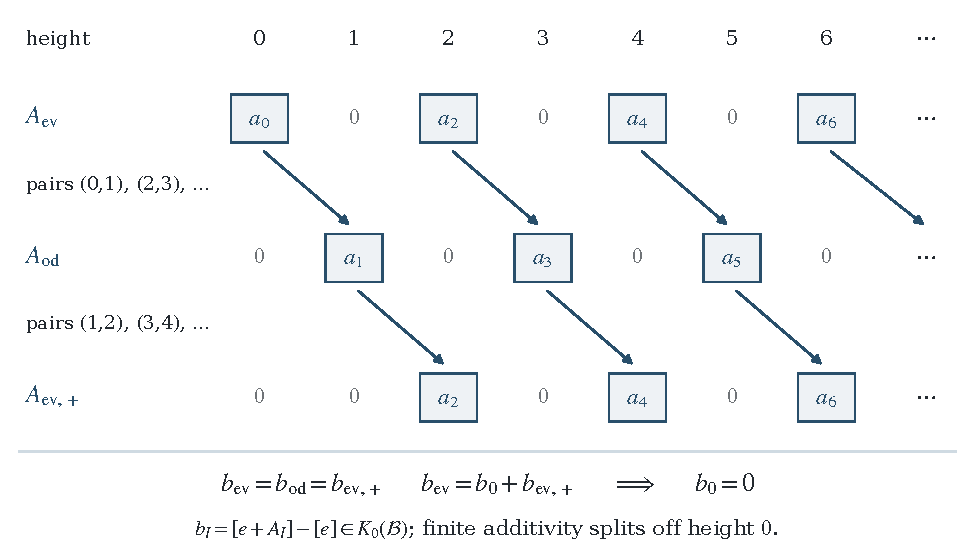
\includegraphics[width=\linewidth]{figures/parity-cancellation.pdf}
  \caption{Height supports of three bounded operator families. Each
  arrow represents the rotation in \eqref{eq:model-pair-rotation}
  followed by rescaling from $a_i$ to $a_{i+1}$. The disjoint pairs give
  the two homotopies. Finite additivity splits off the root family.
  Ellipses describe the supports of actual operators in $\mathcal B$;
  they do not denote an infinite sum of $K$-classes. A zero entry is a
  zero compact difference; the full projection retains its scalar part.}
  \label{fig:parity-cancellation}
\end{figure}

\subsection{The physical root and a supported projection homotopy}

Let $J_{0,\nu}\colon e_{\nu0}^{\mathrm{car}}\mathscr L_\nu
\to\mathscr K_\nu$ be inclusion in its zeroth summand.  If $n_0^B$ is the
number of surviving $\mathscr B_0$ vertices, define the finite operator
\begin{equation}\label{eq:physical-root-row}
 S_\nu=(n_0^B)^{-1/2}\sum_{v\in\mathscr B_0^{\mathrm{surv}}}
               R(t_v^{-1})T_0,
 \qquad v_\nu=S_\nu\chi_0\in A_\nu.
\end{equation}
All sums are finite.  The unrestricted norm of $S_\nu$ need not be uniformly
bounded.  For a source coset $h\HH$, however,
$R(t_v^{-1})\delta_{hf}=\delta_{hft_v}$, so
\eqref{eq:physical-root-row} is exactly the normalized constant transport
in \eqref{eq:assembly-cover-coordinates}, after spreading.  Thus on the
localized source space
\[
 v_\nu=\mathcal J\mathcal I_\nu J_{0,\nu}\chi_0.
\]
Lemma~\ref{lem:assembly-synthesis}, or just its single-height estimate,
gives
\begin{equation}\label{eq:root-row-approximation}
 \|v_\nu-V_\nu J_{0,\nu}\chi_0\|
       \le C_\nu2^{-344.5H_{0,\nu}}\longrightarrow0.
\end{equation}
In particular the $v_\nu$ form a uniformly bounded sequence, because
$\|V_\nu\|\le1$ and $\|\chi_0\|\le1$.  The factor $n_0^B$ has been
accounted for by the multiplicity estimate, rather than suppressed by
assuming that untrimmed sheet summation is an isometry.

Let $a_\nu^{\mathrm{phys}}=a_0(R(z),R(x))$ and let
$p_\nu^{\mathrm{phys}}=e+a_\nu^{\mathrm{phys}}$.
These are fixed-size matrices and the latter are exact projections in
$M_m(A_\nu)$.  Write $a^{\mathrm{phys}}=[(a_\nu^{\mathrm{phys}})]$ and
$v=[(v_\nu)]$ in the reduced quotient, tensoring $v$ with $I_m$ when it
acts on Bott matrices.  The cutoff is real, supported inside the controlled
source carrier, and is one on $\supp a_\nu^{\mathrm{phys}}$.  Equations
\eqref{eq:model-map-near-isometry} and
\eqref{eq:root-row-approximation} imply
\begin{equation}\label{eq:root-supported-isometry}
 v^*v a^{\mathrm{phys}}=a^{\mathrm{phys}}
       =a^{\mathrm{phys}}v^*v,
 \qquad
 \Theta(A_0)=v a^{\mathrm{phys}}v^*.
\end{equation}
For example $v_\nu^*v_\nu-\chi_0^2$ is norm null after restricting to
the cutoff's carrier, and multiplication by $a_\nu^{\mathrm{phys}}$
removes both cutoffs.  The second equality follows by multiplying
\eqref{eq:root-row-approximation} on both sides of the compact difference.
This argument uses a cutoff supported in the larger controlled carrier;
merely asking that a cutoff equal one on the smaller Bott support would not
by itself control its remaining norm.

\begin{lemma}[Supported Bott transport]\label{lem:supported-bott-rotation}
Let $B$ be a $C^*$-algebra, $e\in M_m(\C)$ a projection, and
$a=a^*\in M_m(B)$ such that $e+a$ is a projection in $M_m(B^+)$.
Suppose $v\in B$ is bounded, acts as $v\otimes I_m$ on the matrix factor,
and satisfies $v^*va=a$.  Then
\[
 [e+a]-[e]=[e+vav^*]-[e]\quad\hbox{in }K_0(B).
\]
No contraction assumption on $v$ or identity projection for a carrier is
needed.
\end{lemma}

\begin{proof}
The adjoint relation is $av^*v=a$.  Put $c=\cos t$, $s=\sin t$ and
\begin{equation}\label{eq:supported-bott-path}
 P_t=\begin{pmatrix}
 e+c^2a&cs\,av^*\\cs\,va&e+s^2vav^*
 \end{pmatrix},\qquad 0\le t\le\pi/2.
\end{equation}
It is self-adjoint.  With $W_t=(cI_m,sv)^T$ and
$E_{\mathrm{sc}}=\operatorname{diag}(e,e)$, this is
$E_{\mathrm{sc}}+W_taW_t^*$.  The scalar-factor assumption gives
$E_{\mathrm{sc}}W_t=W_te$.  Moreover
$aW_t^*W_ta=a^2$ and $ea+ae+a^2=a$.  Multiplication now gives
$P_t^2=P_t$.  The endpoints are
$\operatorname{diag}(e+a,e)$ and
$\operatorname{diag}(e,e+vav^*)$, proving the equality after one
fixed stabilization.  All nonscalar entries belong to $M_{2m}(B)$ and the
path is norm continuous.  Its modulus depends only on $\|a\|$ and
$\|v\|$.  In particular it is uniform for bounded coordinate sequences.
\end{proof}

Apply Lemma~\ref{lem:supported-bott-rotation} to
\eqref{eq:root-supported-isometry}.  By
\eqref{eq:model-root-zero} and the homomorphism $\Theta^+$,
\begin{equation}\label{eq:physical-bott-quotient-zero}
 [(p_\nu^{\mathrm{phys}})]-[e]=0
       \quad\hbox{in }K_0(\mathcal Q_r).
\end{equation}
The size in \eqref{eq:supported-bott-path} is $2m$, independently of the
number of transports, graph layers, sheets, or construction index.

\subsection{From the quotient to one finitely generated group}

The remaining two steps recover finite witnesses.  First, equality in the
norm sequence quotient gives equality at every sufficiently late
coordinate.  Then the group elements needed to approximate one such
witness generate the required subgroup.  These are concrete forms of
projection stability and continuity in $C^*$-algebra $K$-theory
\cite[Sections~4.5 and~5.2, Theorem~5.6.1]{Blackadar98}; we give the
witness constructions to keep their finite matrix sizes explicit.

\begin{lemma}[Eventual coordinate equality]\label{lem:eventual-coordinate-equality}
Let $B_\nu$ be unital $C^*$-algebras and let
$P_\nu,Q_\nu\in M_m(B_\nu)$ be projections in a fixed size.
If their classes agree in
$K_0((\prod B_\nu)/(\bigoplus B_\nu))$, then
$[P_\nu]=[Q_\nu]$ in $K_0(B_\nu)$ for all sufficiently large $\nu$.
\end{lemma}

\begin{proof}
The definition of $K_0$ supplies a projection $R$ in a finite matrix algebra
over the quotient and, after finite zero padding, a partial isometry $w$
with
\[
 w^*w=P\oplus R=:E,\qquad ww^*=Q\oplus R=:F.
\]
Lift $R$ to a bounded self-adjoint sequence $r_\nu$.  Its idempotence defect
tends to zero.  On a tail its spectrum avoids $1/2$, and spectral cutting
gives projections $R_\nu$ with $\|R_\nu-r_\nu\|\to0$.  Form the
corresponding $E_\nu,F_\nu$ and lift $w$ to a bounded sequence $b_\nu$.
Set $z_\nu=F_\nu b_\nu E_\nu$.  Then
\[
 \|z_\nu^*z_\nu-E_\nu\|\to0,
 \qquad\|z_\nu z_\nu^*-F_\nu\|\to0.
\]
For large $\nu$ these products are invertible in the respective corners.
The element
$z_\nu(z_\nu^*z_\nu)^{-1/2}$ is a partial isometry with initial
projection $E_\nu$ and final projection $F_\nu$; the latter assertion uses
invertibility in the $F_\nu$ corner.  Thus
$[P_\nu]+[R_\nu]=[Q_\nu]+[R_\nu]$, and cancellation in $K_0(B_\nu)$
proves the result.  Every stabilization used is finite and fixed after the
quotient witness has been chosen.
\end{proof}

\begin{proposition}[Reduced Bott vanishing]\label{prop:reduced-bott-vanishing}
For all sufficiently large $\nu$ in the chosen compatible sequence, the image
of the rank-zero Bott generator of $K_0(\Cr(\langle z,x\rangle))$ is zero integrally in
$K_0(\Cr(\Gamma_\nu))$.
\end{proposition}

\begin{proof}
Apply Lemma~\ref{lem:eventual-coordinate-equality} to
\eqref{eq:physical-bott-quotient-zero}.  At every coordinate
\eqref{eq:physical-bott-profile} identifies the difference with the physical
torus Bott generator.  Equation~\eqref{eq:right-left-regular} transfers the
equality to the usual left reduced algebra without changing the subgroup
elements or their functional-calculus projections.
\end{proof}

\begin{lemma}[A finite witness lies in a finitely generated subgroup]
\label{lem:finite-subgroup-witness}
Let $H\le\Gamma$ be finitely generated, and let $P,Q$ be fixed finite matrix
projections over $\Cr(H)$.  If their images have equal $K_0$ classes over
$\Cr(\Gamma)$, then some finitely generated subgroup $\Ginj$ with
$H\le \Ginj\le\Gamma$ already has $[P]=[Q]$ in $K_0(\Cr(\Ginj))$.
\end{lemma}

\begin{proof}
Choose one finite stabilization projection and a partial isometry witnessing
the equality over $\Cr(\Gamma)$.  Approximate their finitely many entries
by group polynomials, using self-adjoint approximations for the projection.
Adjoin all group elements in these finite supports to generators of $H$;
they generate a finitely generated subgroup $\Ginj$.  The reduced inclusion
$\Cr(\Ginj)\to\Cr(\Gamma)$ is isometric, since restriction of the regular
representation of $\Gamma$ to $\Ginj$ is a direct sum of regular representations
of $\Ginj$.  Thus the required small projection and partial-isometry defects have
the same bounds in $\Cr(\Ginj)$.  Spectral cutting gives the stabilizing
projection in $\Cr(\Ginj)$; compressing the approximate partial isometry to
the two corners and polar-normalizing it gives an exact witness there, just
as in Lemma~\ref{lem:eventual-coordinate-equality}.  Functional calculus
stays inside $\Cr(\Ginj)$.  The original projections $P,Q$ were retained
exactly throughout.
\end{proof}

\section{Compatible choices and the conclusion}
\label{sec:completion}

We choose parameters satisfying all the preceding estimates, then combine
the resulting integral detector and reduced Bott vanishing to prove
Theorem~\ref{thm:main}.  The two indices have different roles:
$i\geq0$ is a height in one infinite
tower; $\nu\geq1$ indexes a sequence of increasingly accurate
constructions.  Degrees are independent of $i$.  No uniform degree
bound in $\nu$ is required.

\subsection{The order of parameters}

First fix the integer $b$ with
$\sqrt{5\cdot2^{1-b}}<3/5$.  This gives the height-independent gap
$\rho=1-.05^2/2$ of Proposition~\ref{prop:sequential-law}.
Retain the explicit compact Bott projection in
\eqref{eq:compact-bott-profile}, its fixed signed class, and
its matrix size.  Fix enlarged support profiles for all neighboring
scales; their ratios depend on $b$, which remains fixed for every
$\nu$.  The rescaling and rotation paths therefore have one common
modulus of continuity.

For each $\nu$, take a target error $\epsilon_\nu\downarrow0$.
Perform the following finite choices in the indicated order.
\begin{enumerate}
\item Choose the constant-extraction length $k_\nu$ from the fixed
gap, so that the term $\rho^{2k_\nu}$ in
\eqref{eq:constant-extraction-error} is sufficiently small.
Choose finite meshes of the two projection paths.  The four endpoint
families, those mesh profiles, and their cutoffs specify a finite
collection of same-height and adjacent-height types.  Choose all
per-factor error tolerances small enough that the telescoping bound
in Lemma~\ref{lem:finite-profile-realization} is below
$\epsilon_\nu$.
\item Choose the finite Fourier truncations and finite matrix-weight
net of Lemma~\ref{lem:product-sampler}.  Its support exponents,
the finite regular-norm test exponent, and the moment constant in
Lemma~\ref{lem:centered-voltage-block} are now fixed.  Also fix a
desired deletion fraction small enough that
$k_\nu\sqrt{\varepsilon_{\mathrm{del}}}$ has the required
error bound.
\item Choose $s_\nu$ as a sufficiently large multiple of $20000$
and $5b$.  Besides the coefficient, probability, and moment
requirements, impose
\[
 \frac{s_\nu}{b}\geq10^{12},\qquad
 \frac b{.50005s_\nu}\leq10^{-6},\qquad
 2^{-.000025s_\nu+O(\log s_\nu)+O_\nu(1)}
       \ll\epsilon_\nu.
\]
The last estimate uses the actual refined alphabet, after the
finite type and weight choices.  Its exponent has a strictly
negative linear term, so it can be imposed along with every
previous finite requirement.  The uniform gate budget and the
height-separation term depending only on $s_\nu,b$ can be made
smaller than the allocated deletion budget at this step.
\item Choose $n_{0,\nu}$, hence
$H_{0,\nu}=(2n_{0,\nu}+1)s_\nu$, sufficiently large.  Impose
$H_{0,\nu}/s_\nu\geq10^{12}$ and all initial-height requirements
in Sections~\ref{sec:labeling}--\ref{sec:assembly}.  In
particular make the remaining separation budget small, make the
sum of the expected pruning fractions smaller than its allocation,
and make the sum of all voltage and norm failure probabilities
less than one.  Increase $H_{0,\nu}$ further to make both the
domain-trimming error and the physical-synthesis error less than
their allocations.  Their bounds have the forms
\[
 C_\nu2^{-345H_{0,\nu}},\qquad
 C_\nu\frac{2^{-344.5H_{0,\nu}}}{1-2^{-344.5b}},
\]
where $C_\nu$ is already independent of height and of this final
increase.  Thus these requirements are compatible.
\end{enumerate}

We explain the choices of random data after these parameters.
Choose the coefficient pools once as in
Lemma~\ref{lem:coefficient-pools}; the same finite pools are reused
on all full blocks.  The sequential law then gives expanding
auxiliary incidences for every table realization in its support.
The deletion estimates in Proposition~\ref{prop:tower-labels}
hold for every such realization.  Proposition~\ref{prop:pruning}
selects a realization with all further layer deletions small.
Only after fixing this old graph apply
Proposition~\ref{prop:sampled-symbols}.  Its one independent
voltage-and-weight law controls both kinds of failure before
their simultaneous avoidance.  There is consequently no change
of measure hidden in the centered moment estimate.

The finite label set is unchanged as heights increase.  It is
refined only by the chosen finite weight net.  The private
completion in Lemma~\ref{lem:private-completion} adds a countable
alphabet, whose coefficients in every operator polynomial are
zero.  The resulting graphical group $\Gamma_\nu$ is countable;
finite generation is obtained from a finite $K$-theory witness
after the quotient argument.

This order also avoids a potential circularity in the norm
sequence quotient.  At stage $\nu$ only finitely many profiles
are required.  Their meshes become finer with $\nu$, and their
uniform modulus of continuity supplies the complete paths in
the quotient.  One does not choose a separate nonuniform
approximation for each height or each path parameter.

\subsection{Proof of the main result}

\begin{proof}[Proof of Theorem~\ref{thm:main}]
Make the sequence of compatible constructions just described.
Proposition~\ref{prop:graphical-realization} embeds $\HH$ in
every $\Gamma_\nu$.
Proposition~\ref{prop:torsion-detector} proves torsion-freeness
and provides an integral class whose evaluation on the ordered
torus $(z,x)$ is $-1$.
Proposition~\ref{prop:reduced-bott-vanishing} proves that, for
all sufficiently large $\nu$, the rank-zero Bott class of this
torus is zero in $K_0(\Cr(\Gamma_\nu))$.

Fix one such $\nu$.  Apply Lemma~\ref{lem:finite-subgroup-witness}
with $H=\HH$ and the physical Bott projections to obtain a finitely
generated subgroup
$\HH\leq \Ginj\leq\Gamma_\nu$ in which that equality already
holds.  The subgroup $\Ginj$ is torsion-free.  Restrict the negative
of the detector class to $B\Ginj$, and denote it by $c$.  Let
$i:\Z^2\hookrightarrow \Ginj$ be the inclusion with ordered
generators $(z,x)$.  The detector evaluation is unchanged by restriction,
so
\[
 \ip{(Bi)^*c}{[T^2]}=1,
 \qquad i_*(\beta)=0\quad\hbox{in }K_0(\Cr(\Ginj)).
\]
It remains to detect the corresponding geometric class and identify its
assembly image.  We use compactly supported $K$-homology throughout. On finite CW
complexes, the natural comparison of geometric cycles with analytic
$K$-homology sends $(M,E,f)$ to $f_*[D_E]$
\cite[Theorems~6.1--6.2]{BHS07}; passage to finite-subcomplex colimits
gives the convention used for $B\Ginj$. In particular the compact torus
cycle used here defines a class without any compactness assumption on
$B\Ginj$.

Let $L$ be the line bundle on $B\Ginj$ classified by $c$. The naturality
of the index pairing follows at a finite stage from pullback of vector
bundles and associativity of the Kasparov product:
\[
 [L]\otimes f_*[D]=[f^*L]\otimes[D],\qquad f=Bi.
\]
The same identity holds for the virtual bundle $[L]-[1]$. Applying the
twisted spin Dirac index theorem \cite{AS63}, in the dimension-two form
of \cite[Theorem~1]{BvE16}, gives
\begin{align*}
 \bigl\langle [L]-[1],(Bi)_*[D_{\mathbb T^2}]\bigr\rangle
 &=\operatorname{index}(D_{\mathbb T^2}\otimes (Bi)^*L)
       -\operatorname{index}(D_{\mathbb T^2})\\
 &=\bigl\langle (Bi)^*c,[\mathbb T^2]\bigr\rangle=1.
\end{align*}
The torus tangent bundle is trivial, its $\widehat A$ class is one,
and its untwisted complex Dirac index is zero. Thus the pushed-forward
$K$-homology class has infinite order and is nonzero after tensoring with
$\Q$.

Under Fourier transform $\Cr(\Z^2)\cong C(\mathbb T^2)$, the assembly
image of the torus spin Dirac class is the rank-zero Bott generator, up to
orientation. This is the full-torus case of Emerson--Hudson's assembly
formula for a $K$-oriented subtorus \cite[Theorem~1.3]{EH20}: the dual
subtorus is a point, whose shriek class is the compact Bott class.

For completeness we verify the required subgroup naturality at this
particular cycle. Put $A=\Cr(\Z^2)$, $B=\Cr(\Ginj)$, and write
$j:A\to B$ for the isometric inclusion. If $P\to T^2$ is the principal
$\Z^2$-bundle classified by the torus map, its Mi\v{s}\v{c}enko bundle
is $E_A=P\times_{\Z^2}A$. The bundle obtained after the subgroup map is
canonically
\[
 (P\times_{\Z^2}\Ginj)\times_{\Ginj}B
 \cong P\times_{\Z^2}B
 \cong E_A\otimes_j B.
\]
The last identification sends $([p,a],b)$ to $[p,j(a)b]$; the balancing
relations and fiber inner products agree because $j$ sends each subgroup
unitary to the same group unitary. Extension of coefficients therefore
commutes with the index Kasparov product. In explicit notation,
\[
 \bigl([E_A]\otimes_{C(T^2)\otimes A}([D_{T^2}]\boxtimes1_A)\bigr)
      \otimes_A[j]
 =[E_A\otimes_j B]\otimes_{C(T^2)\otimes B}
      ([D_{T^2}]\boxtimes1_B).
\]
These indices are the assembly classes by the Mi\v{s}\v{c}enko comparison
\cite[Corollary~1.4 and diagram~(1.6)]{KP22}; see also
\cite[Proposition~3.7 and Theorem~4.1]{Land15}.
The comparison applies to the compact torus cycle, and its
finite-subcomplex colimit handles the target $B\Ginj$.
Consequently
\[
 \mu_{\Ginj}^r\bigl((Bi)_*[D_{T^2}]\bigr)
   =j_*\mu_{\Z^2}^r([D_{T^2}])=0
\]
by Proposition~\ref{prop:reduced-bott-vanishing} and
Lemma~\ref{lem:finite-subgroup-witness}. This is integral vanishing,
whereas the index pairing above proves infinite order of the source class.
\end{proof}

\bibliographystyle{plain}
\bibliography{references}
\end{document}
